\documentclass[11pt,oneside,notitlepage]{report}
\usepackage{fullpage}
\usepackage[pdftex,
            pdfauthor={Jeffrey Yoo Warren},
            pdftitle={Grassroots Mapping: a toolkit for participatory and activist cartography},
            pdfsubject={Participatory Cartography},
            pdfkeywords={Cartography},
            pdfproducer={Latex with hyperref},
            pdfcreator={pdflatex,colorlinks}]{hyperref}
\usepackage{graphicx,wrapfig,color,pdfcomment,booktabs,ctable,textcomp,tabularx,array,acronym,threeparttable}
\usepackage[table]{xcolor}
\usepackage[hang,small,bf,margin=0.5cm,tableposition=top]{caption}
\usepackage[ragged]{footmisc}
\newcommand{\otoprule}{\midrule[\heavyrulewidth]}
\definecolor{linkblue}{rgb}{0.2,0.2,1}
\hypersetup{colorlinks=true,
	    urlcolor=linkblue,
	    citecolor=linkblue,
	    linkcolor=linkblue}
\newcolumntype{Y}{>{\raggedright\arraybackslash}X}
\newcolumntype{W}{>{\raggedleft\arraybackslash}X}

\definecolor{tableShade}{HTML}{EEEEEE}

%% Define a new 'jeff' style for the package that will use a smaller font.
\makeatletter
\def\url@jeffstyle{%
  \@ifundefined{selectfont}{\def\UrlFont{\sf}}{\def\UrlFont{\small\ttfamily}}}
\makeatother
%% Now actually use the newly defined style.
\urlstyle{jeff}

\begin{document}
\hfuzz2pt % don't report overfull if within 2 pt



\title{\begin{flushleft}\vspace{-40px}
Grassroots Mapping: tools for participatory and activist cartography\\ \vspace{10px}
\emph{by Jeffrey Yoo Warren}\\ \vspace{10px}
\large{B.A. Yale University 2006}\\ \vspace{30px}
\large{Submitted to the Program in Media Arts and Sciences,\\
School of Architecture and Planning,\\
in partial fulfilment of the requirements for the degree of\\
Master of Science\\
at the {\sc MASSACHUSETTS INSTITUTE OF TECHNOLOGY}\\
September 2010\\ 
\copyright 2010 Massachusetts Institute of Technology. All rights reserved.}\\
\vspace{30px}
\large{\emph{author: }}\\ \vspace{2px}
\hrule \vspace{10px}
\begin{flushright}
Program in Media Arts and Sciences
September 2010
\end{flushright}
\vspace{10px}
\large{\emph{certified by: }}\\ 
\hrule \vspace{10px}
\begin{flushright}
Dr. David Small\\
Associate Professor\\
Program in Media Arts and Sciences\\
Thesis supervisor
\end{flushright}
\vspace{10px}
\large{\emph{accepted by: }}\\
\hrule \vspace{10px}
\begin{flushright}
Chris Csikszentmihalyi\\
Research Scientist\\
Director, Center for Future Civic Media and Computing Culture Group\\
MIT Media Lab\\
\end{flushright}
\vspace{20px}
\large{\emph{accepted by: }}\\
\hrule \vspace{10px}
\begin{flushright}
Dr. Mitchel Resnick\\
Professor\\
Program in Media Arts and Sciences
\end{flushright}
\end{flushleft}}
\date{}
\author{
%Jeffrey Warren
}
\maketitle

\setlength{\parindent}{0pt}
\setlength{\parskip}{0.8em}

\Large{Grassroots Mapping: tools for participatory and activist cartography \vspace{10px} \\ 
\emph{by Jeffrey Warren}\vspace{10px} \\ 
B.A. Yale University 2006} \vspace{20px} \\ 
\large{Submitted to the Program in Media Arts and Sciences,\\
School of Architecture and Planning,\\
in partial fulfilment of the requirements for the degree of\\
Master of Science\\
at the {\sc MASSACHUSETTS INSTITUTE OF TECHNOLOGY}\\
September 2010\\ 
\copyright Massachusetts Institute of Technology 2010. All rights reserved.}\\ \vspace{20px}

\normalsize{
\section*{Abstract}



}

\vspace{20px}
\large{
Thesis supervisor:\\
Dr. David Small\\
\emph{Associate Professor}\\
Program in Media Arts and Sciences\\
}

\pagebreak

\normalsize{
\section*{Acknowledgements}
}

\tableofcontents

\chapter{Introduction}

\section{Defining Grassroots Mapping: tools, practices, or community?}

Exactly what makes up the Grassroots Mapping project? Is it a body of code, available under an MIT license at \url{http://github.com/jywarren/cartagen}? Is it a set of mapping practices, or tools, which have been employed in Lima, Peru, or Rio de Janiero? Or is it a community of practitioners and the web site, wiki, and mailing list which tie them together?

Fundamentally this project is intended to make the process of mapmaking easier for lay users, with the intent to broaden participation in cartography. Throughout much of the world, maps can be seen as a tool of the state and of industry to express control over world we live in. By simplifying the means to create maps, from the data gathering through the editing and publication of digital and print maps, the tools and techiques I have created are designed to further democratize cartography. In turn, it is hoped that the ability of a broader public to make maps at a reasonable cost will help to empower bottom-up cartographic activism and to circumvent the current power structure of map-making. 

The core of the Grassroots Mapping project is the \textbf{application} of a novel combination of technology to specific communities. The technology consists of low-cost aerial imaging techniques using balloons and kites to take photos from the air, and a novel online tool for stitching the resulting imagery into maps. The success of these tools is due to the effort and faith of the organizations and individuals who were willing to adopt these new and unfamiliar tools, and who saw their potential for use in their communities in Lima, Peru, and the oil spill crisis on the coast of the Gulf of Mexico. This includes Carla del Carpio of Manzanita "A" and Ernesto Fernandez of CEDRO, both in Lima, Peru, and Daniel Miracle and others from Escuelab, also in Lima. It includes Kris Ansin, Shannon Dosemagen, and Anne Rolfes of the Louisiana Bucket Brigade in New Orleans. It also includes the dozens of participants who tirelessly flew kites and balloons, and untangled and wound miles of string day after day. Perhaps most importantly, the tools grew and evolved in response to sustained use by participants, and with the input and collaboration of those who used them.

\subsection{Uses of aerial imagery}

Participants in the project have made maps for diverse purposes, including environmental monitoring, tenure rights, journalism, and commercial use. Many maps were created in the context of youth workshops emphasizing hands-on learning and community planning, and the tools' unique ability to produce on-demand maps was explored in crisis situations and areas of conflict. Due to their low cost, the techniques have potential for even broader use in asset mapping in low-income or developing areas, and local-level urban planning. The ability to see one's home from above can prompt thought and discussion about community, environment, and social issues. By engaging with and teaching local communities to use the tools, they have taken on a more personally relevant meaning than efforts which charactarize themselves as remote sensing. 
 
\subsection{Grassroots Mapping as pedagogy}

To enable widespread adoption, the project evolved to include a variety of teaching materials, printed guides, online videos, and workshops, both by myself and by the diverse collaborators who took ownership of the tools. These materials spanned a broad range of audiences, from 10-15 year olds in Lima, Peru to environmental activists in West Virginia and Kentucky. 

This documentation evolved as I collaborated with and instructed participants in dozens of workshops over the past year. These occurred in diverse contexts, from a two week high school workshop at Beaver Country Day School in Chestnut Hill, outside of Boston, to an hour-long teaching session in City Park, New Orleans, for volunteers mapping the April 2010 BP Oil Spill. 

\subsection{Grassroots Mapping as a community}

Ultimately, even the digital tools, including the Cartagen map rendering framework and the Cartagen Knitter, a tool for orthorectifying aerial imagery, were built with assistance and support of UROPs, colleagues, and contributors in the broader mapping community. That this has become the norm in technology projects does not detract from the fact that much of this work would have been impossible without such contributions. 

Building tools is unlike developing more abstract technologies in that to be successful, a series of compromises and pragmatic decisions must guide the design process, as well as continuous communication with an audience of users. The Grassroots Mapping project has evolved inresponse to these needs and should be examined in the context of the specific uses it has attempted to address, rather as an isolated or 'pure' work.

\section{Tools, technologies, and audience}

The tools developed as part of the Grassroots Mapping project address the needs of both committed enthusiasts who need powerful and efficient mapping technology, as well as those who have little experience and expertise but need simple and direct tools to make maps. Therefore, some of the tools, while being simple to use, are intended for `power users' or those technically fluent in writing and editing code. The Cartagen framework falls under this category. Other tools, such as the balloon and kite platforms for capturing aerial imagery, are intended for a wider audience, as is the Cartagen Knitter, a specific use of the Cartagen framework. A description of the various tools follows.

The Grassroots Mapping Kit can be used to capture original aerial imagery, process and stitch the results, and publish digital and print maps. This section focuses on the framing, intent, and audience of the necessary tools. A technical discussion of the tools can be found in Chapter \ref{chap:toolchain}. 

\begin{table}[tp] 
\caption{Grassroots Mapping workflow}
\centering %
\renewcommand{\arraystretch}{1.4}
\begin{tabularx}{\textwidth}{YYY}
\toprule
Capture&Orthorectification&Publication\\\otoprule
2-3 people can map several square km in 1 day&Sorting photos can take \textgreater1 hour, stitching up to 1 day&Export from Cartagen Knitter generates a TMS or printable GeoTiff; only web access is needed.\\\bottomrule 
\end{tabularx}
\end{table}

Briefly, map-makers visit the site they intend to map, bringing with them a kite, a balloon, a helium tank, a digital camera, and a minimum of 200 meters of string, along with an assortment of other materials. Attaching the camera to the tethered balloon or kite, they capture imagery by setting the camera to automatically take pictures at a 1-10 second cycle and raising it to between 200 and 2000 meters in altitude. The map-makers reel in the tether to recover the imagery and, retiring to a web-enabled computer, upload the best imagery to the Cartagen Knitter web site.\footnote{\url{http://cartagen.org/maps/}} There they create a new online map, and using either OpenStreetMap vector data or a tiled map base layer for reference, each imagery is orthorectified. The resulting map can be embedded in another website for online viewing, exported as a \ac{TMS} service, or printed from a \ac{GeoTIFF}, depending on the intended use. 

The Grassroots Mapping Kit and associated techniques are thoroughly documented at the project wiki, at \url{http://wiki.grassrootsmapping.org}, and additional support and discussion is available at the project mailing list and blog, which can be found at \url{http://grassrootsmapping.org} along with extensive documentation of past and in-progress mapping efforts around the world. Printed documentation is also available in the form of available in the form of a 5-page illustrated guide and several checklists designed to accompany each kit.\footnote{See \ref{sec:guide}}

\chapter{Movements towards a participatory and activist cartography}

A brief description of three distinct groups of practitioners is worthwhile, as each embodies a distinct conception of map-making and its purpose. These three cartographic movements have positioned themselves as challengers to existing forms of cartography, and as such, the following will help to situate the Grassroots Mapping project (in addition to the Cartagen framework) as a similar attempt to broaden participation and reconceptualize the practice. 

\section{Experimental geography, radical cartography}

A growing movement toward a cartographically literate art practice has emerged which seeks to use cartographic tools and attitudes in a critical and activist manner. Some groups, such as Proboscis, take explicit inspiration from Guy Debord's psychogeographic movement of the 1950s. Others such as the Center for Urban Pedagogy, use map-making as a means to explore social and environmental ills in a participatory manner. What these practitioners have in common is that they have begun to appropriate tools and techniques from professional cartography, but to apply them towards new, and often more socially and politically engaged ends. 

Artists like Bill Rankin use the thin-lined mechanical aesthetics of GIS to comment upon the normally cartographically invisible American Indian reservations, emphasizing the incompatiblity between such modes of representation and the more complex geographies which actually exist in the world. His map, `The United States?' offers two separate attempts, but Rankin points out the difficulties in such an adaptation of techniques:

\begin{quote}
At stake here is the European definition of nation-state sovereignty, which implies a close (and, ideally, consensual) relation between an area on a map and the governance of its inhabitants. It is not simply that a European-style map has a hard time representing the sovereignty rights (or claims) of indigenous peoples; rather, such relations are a priori impossible to depict on a typical map. \cite{rankin2003reservations}
\end{quote}

The collective Hackitectura inverts a map of the Gibralter area with Morocco and Western Sahara on top and Spain and Portugal below, while highlighting the complex landscape of legal and illegal immigration. Graphs, diagrams of security systems, and satellites dot the map depicting `the multitude versus the Empire', along with marks for immigrant detainment and the Spanish tomato farms whose need for cheap labor feeds much of the migration. The map-makers' willingness to abandon the guise of objectivity in favor of such a clear geopolitical agenda is typical of many members of this wider cartographic movement.  

\begin{figure}[h]
	\begin{center}
		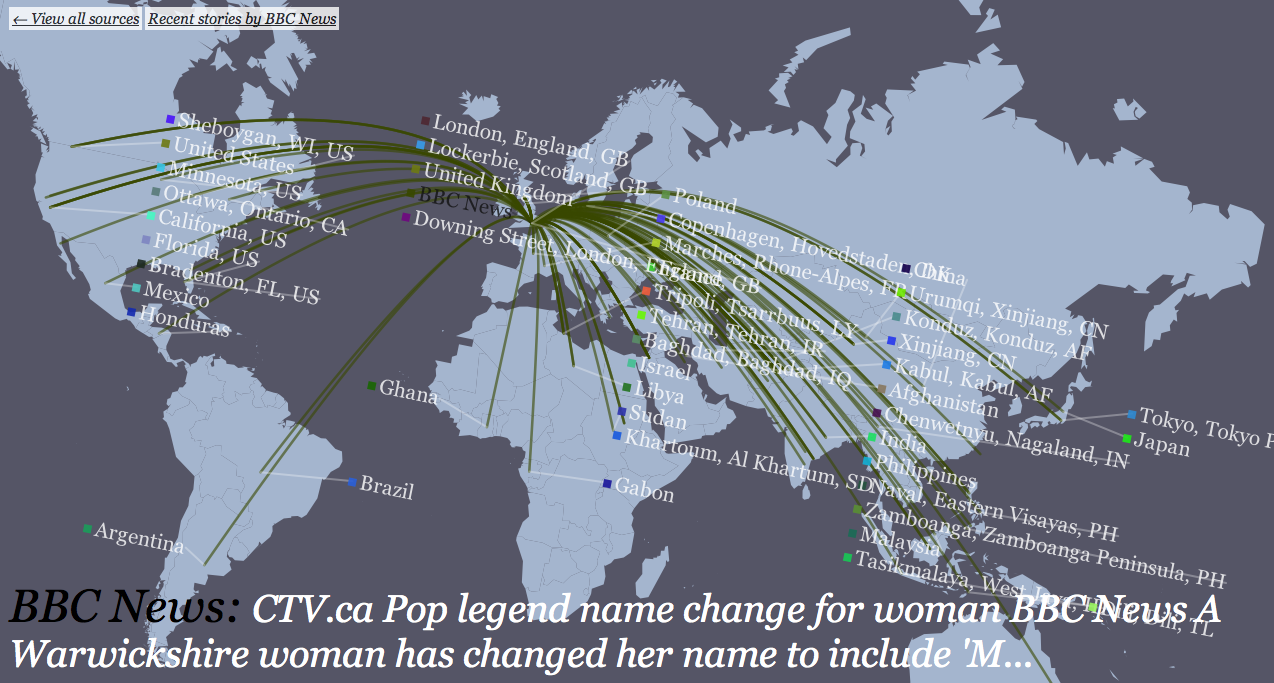
\includegraphics[width=1\textwidth]{images/newsflow.png}
		\caption{A selection of articles published by the BBC, linked to the BBC headquarters in my project NEWSFLOW, 2009}
	\end{center}
\end{figure}

Proboscis in particular has produced a number of works with urban communities with the goal of helping people `articulate and share their xperiences of inhabiting the city' and `become co-creators and not just consumers of information' --- the latter of which parallels the neogeographers' interest in making participants of their audience (See Section \ref{sec:neogeography}). Their projects take the form of map-making workshops and activities, using paper as well as GPS-enabled mobile phones. They focus on recording the historical narratives of participants while relating the stories to geographic positions and routes in a kind of city-wide game. 

Proboscis uses the term `bodystorming' to describe their methodology, wherein `the transformation of abstract ideas and concepts into physical experiences, a tactile approach allowing us to investigate different qualities that ideas may have when applied to physical settings --- part of a dynamic and continuous process of trial and error.' \cite{proboscis2003bodystorming} 

%A People's Atlas of Chicago

%Proboscis: Urban Tapestries... democratization of GIS tools for an `anthropology of ourselves'

%Lots of work by Proboscis: \href{http://urbantapestries.net/}{Social Tapestries/Urban Tapestries}, 2002-7 - Urban Tapestries investigated how, by combining mobile and internet technologies with geographic information systems, people could `author' the environment around them; a kind of Mass Observation for the 21st Century. Like the founders of Mass Observation in the 1930s, we were interested creating opportunities for an `anthropology of ourselves' – adopting and adapting new and emerging technologies for creating and sharing everyday knowledge and experience; building up organic, collective memories that trace and embellish different kinds of relationships across places, time and communities.

My own project ARMSFLOW (\url{http://armsflow.org}, 2007) describes in map form the sale of conventional arms between governments worldwide from 1950-2006, using data culled from the Stockholm International Peace Research Institute, or SIPRI. Red lines of varying thickness (representing an abstract metric called TIV, or trend-indicator value) link buyers to sellers, and users may explore the data by country or by year. A followup project, NEWSFLOW (\url{http://newsflow.cartagen.org}, 2009), displays in a similar format connections between news organizations and the locations of stories they publish, as scraped from Google News. Though visually compelling and information-rich, the shortcomings of these two maps are emblematic of the `data visualization' movement; Natalie Jeremijenko addresses the crux of the matter when she questions their sources: 

\begin{quote}
...the designers of these types of projects use extant data sets from the EPA, from the Toxic Relief Inventory, federal databases, and do so without criticism, without asking how the data is generated, who collected it and under what conditions. That is, what does the data actually represent? \cite{jeremijenko2008situated}
\end{quote}

This criticism was revelatory to me, and led to my increased interest in engaging participants not only in interpreting information, but in creating information. By augmenting the literacy and ability of individuals to capture, author, and frame the acquisition of new data, we engage a broader public at the level of researcher and of investigator. Rather than playing solely the interpretive role of the designer or editor, I have attempted to insert participants further upstream --- closer to the source --- with the intent of gaining greater leverage in the construction of geography. 

\href{http://www.sciencedirect.com/science?_ob=ArticleURL&_udi=B6VG2-4XHJX4B-1&_user=10&_coverDate=08/31/2009&_rdoc=1&_fmt=high&_orig=search&_sort=d&_docanchor=&view=c&_searchStrId=1186930669&_rerunOrigin=google&_acct=C000050221&_version=1&_urlVersion=0&_userid=10&md5=a9327ffa62e089e863f892a4551c1717}{Intervention: Mapping is critical!} - This intervention targets the much heralded demise of the map in geography and the recently proposed “rethinking” of maps. It comprises contributions from two political geographers, a military geographer, a political scientist, and two activist cartographers and argues that there is not so much a need to “rethink” maps, but to “re-engage” with the material practices of mapping, and above all to “re-make” maps.

\section{GIS practitioners}
\label{sec:gis}

Professional map makers have used Geographic Information Systems, or GIS since the 1960s, which in recent decades has increasingly centered on the ArcGIS suite by ESRI. More recently, GIS as a methodology has met with some criticism amongst newer generations of digital map-makers for its widespread use of expensive proprietary tools such as ArcGIS, both for their cost and because such tools present a high barrier to non-expert participation due to their complex interfaces. However, it is easy to forget that GIS were created as part of a movement towards a more participatory and interactive cartography, by reducing the costs and increasing the abilities of users to manipulate and publish geographic data.

Another, parallel movement known as `critical GIS' but encompassing several groups such as Qualitative GIS, Feminist GIS, Participatory GIS and Public Participation GIS evolved starting in the 1990s with roots in human geography as well as amongst GIS practitioners themselves. These critical GIS proponents have challenged traditional GIS practice from a humanist perspective, for its failure to incorporate non-quantitative sources, and for its `potential for exclusion and disempowerment' \cite{elwood2009qualitative}. Other proponents of a Qualitative GIS such as Marianna Pavlovskaya have assaulted the quantitative basis for GIS, pointing out amongst other reasons that much of GIS usage relies on spatial imagination and intuition, as in many visual examination-based techniques. She notes that most GIS software ships with only basic spatial analysis capabilities, and suggests that the high reliance on human reasoning in typical usage has been obscured by `unfriendly user interfaces'. Most importantly, Pavlovskaya draws attention to the fact that the most common output of GIS use is in visualizations, designed for `visual impact', and as such emphasize heuristic interpretation over quantitative. \cite{pavlovskaya2009nonquantitative} 

Instead, critical GIS proponents argue that GIS is primarily a power relation, due to its association with authoritative quantitative analysis and the `fascination of Western science and geography with vision, seeing, and looking as a primary and supposedly objective way of knowing, which is in fact partial, embodied, and masculinist.' \cite{pavlovskaya2009nonquantitative}\footnote{See Section \ref{sec:truth}.} The resulting image of `GIS as a powerful juncture of science, technology, and authority' \cite{pavlovskaya2009nonquantitative} leads to an exclusivity that places the benefits of geospatial information and technology beyond the reach of the public and in the hands of those already in power. Pavlovskaya and her colleagues advocate a broader and more inclusive practice of cartography which incorporates anthropological and `mixed methods' methodologies --- including photographs, community-produced paper maps, and `3D model mapping' where participants construct multimedia scale models of their communities in a discursive and process-focused activity. 

These attempts to reconceptualize GIS practice have matched well with the work of participatory or public participation GIS (PGIS) researchers who have --- often in developing countries, or with indiginous groups --- sought to develop more inclusive map-making activities to address these criticisms of conventional GIS. These have included ground mapping, performed in an outdoor area using stones or flags to create scaled maps, and relief model mapping using three dimensional cardboard contour maps annotated with pins and labels.\footnote{A discussion of the challenges the PGIS movement has faced can be found in Section \ref{subsec:pgisshortcomings}.} As Robert Chambers remarks, PGIS techniques have met with widespread adoption and success across the world, due to their `power and versatility... the relative ease with which it can be facilitated, the fun, fulfilment and pride which people derive from it, and its multiple uses by so many stakeholders'. \cite{chambers2006whose}

Despite sharing many of the same goals of inclusive, participatory techniques, an emphasis on making the audience into producers of information, and inexpensive tools designed for non-experts, neither the critical GIS movement nor the experimental geography movement widely collaborated with or even communicated with the following group, which from a technological perspective has perhaps the greatest potential to innovate new tools and techniques. 

\section{Neogeography}
\label{sec:neogeography}

With the rise of web-based data and display systems came a group composed primarily of entrepreneurs, programmers and web designers, who have adopted the name \emph{neogeographers}. This group positions itself in contrast to traditional approaches such as GIS, and favors open data sharing, standards-based data formats. Neogeographers advocate a kind of `people's GIS', and has have worked to develop a set of free and open source software tools to replace proprietary solutions. The neogeographic movement, though it might have found its roots in the opening of the Google Maps API (see Section \ref{sec:webmapping}), focuses today on largely web-based software such as OpenLayers, Mapnik, and GeoDjango. Some downloadable map viewing and editing packages such as QGIS or JOSM are also available, though even these are often used to produce data for web publication. The availability of a relatively complete open-source toolchain for authoring and publishing maps is a result of the gradual shift away from easy-to-use commercial APIs. \cite{rana2009neogeography} However, some services such as Google's geocoding API, Yahoo's Placemaker API, and a variety of commercial satellite imagery sources, are still relied upon --- generally because they outperform open-source alternatives. In some cases, equivalent open alternatives are nonexistent or not widely known.

One identifying theme in the neogeography movement is the shift of users from consumers to producers of maps, though primarily in the online world. \cite{oconnor2008maps} The ability to create and publish map data using simple and free tools has dramatically broadened participation in map making, and Rana and Joliveau suggest that neogeography rejects the `prescribed role/interaction between the four main components, namely the audience, the information, the presenter and the subject...'. \cite{rana2009neogeography} Neogeographers prefer `crowdsourced' data, contributed by collaboration and volunteerism, to proprietary data, which they have come to distrust due to copyright, access, and format limitations. Data produced by the public and liberally licensed for public use, may be translated, republished, remixed, and repurposed without parasitic reliance upon large and often uninterested organizations and governments. 

Another important aspect of the movement is that the creators of neogeographic software tools typically do not have a formal or academic background in geography or GIS, but from a programming and software engineering background. This has some technical benefits, in that the solutions they promote and develop are often conceived of from a novel perspective, sometimes resulting in higher performance, broader applications, and reconcetualizations of both what and \textbf{for whom} maps are for. It has also resulted in an `outsider' attitude amongst neogeographers, and even some resentment from traditional GIS practitioners; this has played an important role in how the movement presents itself to the rest of the world, and what choices it makes in the development of tools. For example, the OpenStreetMap project, discussed at length in Section \ref{sec:openstreetmap}, was developed in response to the restrictive crown copyright of the British Ordnance Survey national map. \cite{chilton-crowdsourcing}, and was eventually 

While neogeography shares many of the goals of the PGIS movement, relatively little communication exists between these two factions due to their different origins and mutually isolated venues for publication.\footnote{An exception is Mikel Maron's efforts in Kibera, among other places, which makes explicit reference to PGIS practices..... reference} Rana et all describe neogeography as an `outcome of the increasingly close integration of our lives with geocomputational and World Wide Web technology.' That statement may be more accurate if `our lives' refers to the lives of neogeographers, or at most refers to that thin slice of the global population which knows what an API is, or owns an iPhone. As discussed in Chapter \ref{chap:need}, most of the world has little or no access to digital geospatial services and information, and this may account for the mounting interest in such tools' application in areas of crisis or humanitarian need. In the last few years, we see an increasing number of neogeographers engaging in socially or politically engaged work --- groups such as the Humanitarian OpenStreetMap Team, Washington-based firm DevelopmentSeed, NiJeL, Ushahidi, and many more. Many of these have formed partnerships with larger and older organizations such as the World Bank and even the United Nations. A more in-depth examination of such works and the relevant technologies was published in 2008 by Sean O'Connor and the Tactical Technology Collective under the name `Maps for Advocacy'. \cite{oconnor2008maps} 

\chapter{Subjectivity in Mapping}
\label{chap:subjectivity}

The need for a more participatory cartography is predicated on the exclusion of many from the practice of map-making as it stands today. Even more importantly, it depends on the point of view that mapping is an inherently non-neutral practice, and that for maps to serve wider and more democratic interests, it must accommodate diverse viewpoints. Maps serve interests, and understanding their role not as documentation of what makes up the world, but as rhetorical, tactical, and \emph{subjective} tools is an important prerequisite to what this document argues.

\begin{wrapfigure}{r}{0.5\textwidth}
	\begin{flushright}
		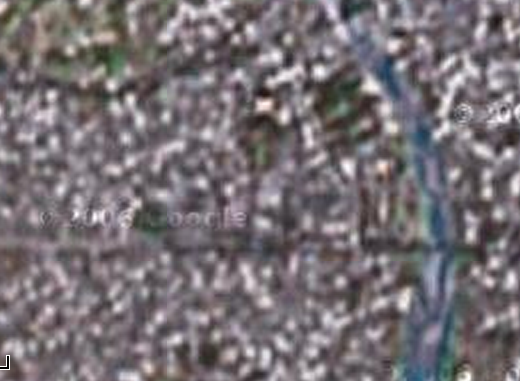
\includegraphics[width=0.45\textwidth]{images/kutaisi.png}
	\caption{Kutaisi, the second largest city in Georgia. Google Maps, July 2010}
	\end{flushright}
\end{wrapfigure}

\section{The mythical `complete map'}

One common sentiment often heard in contemporary map literature is that the earth is more or less completely mapped. The availability of satellite imagery in tools like Google Earth, and the ability to zoom shockingly far into a dizzying array of places, from power plants in North Korea to the top of Macchu Pichu, gives the casual user the impression that we have indeed created a complete map of the world. However, if one attempts to find imagery of places which are removed \textbf{socioeconomically}, it becomes clear that while there may not be many \textbf{blank} spots on the map, there are an abundace of \textbf{blurry} spots. 

This of course sidesteps the fact that an aerial image does not a map make --- that is to say, in order to take advantage of the many applications of geographic data, vector maps which geometrically and semantically describe features must exist, including labels, tags, metadata, and even parseable relations -- from which driving routes may be calculated. These are almost entirely absent from many areas of the world (see Chapter \ref{chap:need}). Amongst cartographers, the idea that maps accurately, or even completely depict a location is not entertained in a literal sense, yet there persists a sense that complete maps are possible. Within certain realms, communities such as OpenStreetMap have declared completion, as in an email by Etienne Cherdlu to the project's developer mailing list in 2006, entitled `UK Motorways 100\% Complete': \begin{quote}I'm pleased to announce that the main carriageways of all mainland UK motorways have been completed. Over 3,000 km of roadway.\end{quote}

\begin{wrapfigure}{r}{0.5\textwidth}
	\begin{flushright}
		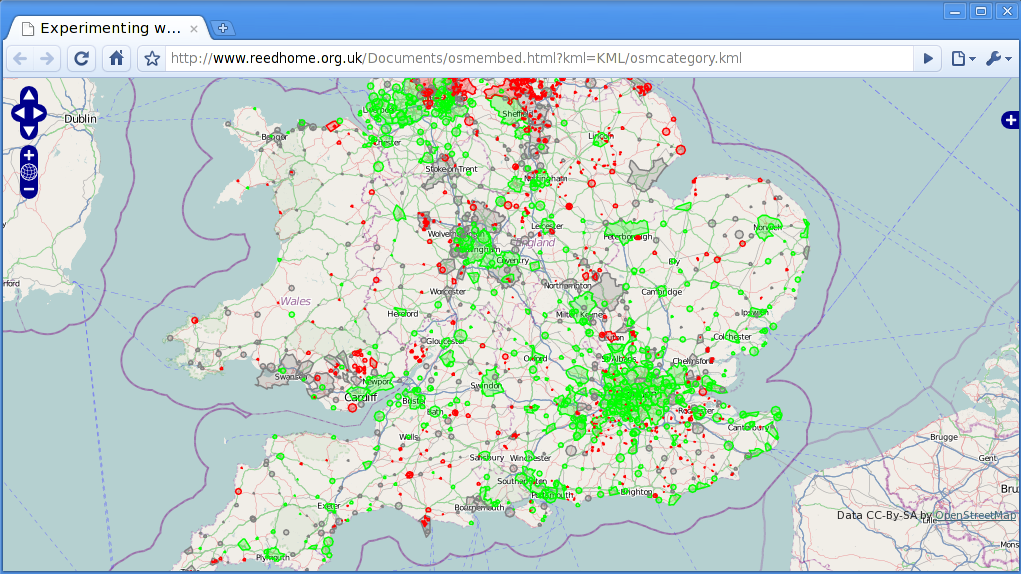
\includegraphics[width=0.45\textwidth]{images/osm-missing-parts.png}
	\caption{A map depicting all `incomplete' areas of OpenStreetMap in the UK. (\url{http://www.reedhome.org.uk/Documents/osmembed.html?kml=KML/osmcategory.kml})}
	\end{flushright}
\end{wrapfigure}

Still, OpenStreetMap's tagline describes the project as an 'editable map of the whole world', and the scope of the project is growing. The inclusion of increasingly subjective data has transformed the project, from road conditions to contested political boundaries such as the borders of Palestine or the existence of Western Sahara as a sovereign nation, to the possibilities of including indoor features such as rooms and hallways. Yet the premise of mapping the entire planet should remain an obvious fantasy; in fact, the fiction of such a complete map has been explored by several authors, most notably in a short story by Jorge Luis Borges and Adolfo Bioy Casares, called `On Exactitude in Science':

\begin{quote}
...In that Empire, the craft of Cartography attained such Perfection that the Map of a Single province covered the space of an entire City, and the Map of the Empire itself an entire Province. In the course of Time, these Extensive maps were found somehow wanting, and so the College of Cartographers evolved a Map of the Empire that was of the same Scale as the Empire and that coincided with it point for point. Less attentive to the Study of Cartography, succeeding Generations came to judge a map of such Magnitude cumbersome, and, not without Irreverence, they abandoned it to the Rigours of sun and Rain. In the western Deserts, tattered Fragments of the Map are still to be found, Sheltering an occasional Beast or beggar; in the whole Nation, no other relic is left of the Discipline of Geography.
\cite{borges1946exactitude} \footnote{The idea of a 1:1 map of a whole country was originally mentioned in Lewis Carroll's novel \textbf{Sylvie and Bruno Concluded}.} 
\end{quote}

Beyond the technical impossibility of total mapping lies the trend towards increasingly individualistic, subjective, and divergent models of the world, which inevitably occur as maps become more universal and more detailed. Rather than pursuing the goal of a single canonical representation of the planet and all of its conflicting interpretations, participatory map-making should embrace diversity, and allow for separate but related means of describing the world. \footnote{My belief in the value of a divergent paradigm for digital mapmaking was also the impetus for my development of the Cartagen web mapping framework, which shifts the interpretation and rendering of map feature data to the client side (rather than generating a single canonical server-side rendering), allowing for endless variety of representation.} 

\section{A `ground truth' policy for collaborative map-making}

OpenStreetMap has in fact begun to encounter a number of challenges due to the inherently subjective nature of map-making --- especially as the project has grown to encompass dozens of countries, cultures, and socio-political perspectives. Due to the project's open and wiki-like architecture, occasional disagreements occur between users, and a convention has been established to resolve such disputes. OpenStreetMap can accommodate an unlimited number of language translations for the label of a map feature, but the \textbf{default} label is what is displayed on the web map at OpenStreetMap.org. The `on the ground' policy, as it is known, places any editorial decision in the hands of `the people on the ground at that location'. The policy, whose definition was led by Mikel Maron, was originally proposed in response to an `edit war' in 2007 between Turkish-speaking mappers from northern Cyprus and Greek-speaking mappers from southern Cyprus. \cite{osm2007disputes} While such a policy has in general served the project well, its necessity is an indication that as map-making becomes a more widespread and inclusive practice, the increasing diversity of viewpoints will make a single canonical map less feasible. 

\subsection{Privacy and mapping, privacy and open geodata}

Privacy is of course yet another reason to shy away from total mapping. Indeed, for any publicly available map to include such details as the positioning of my coffee table or wifi router \footnote{A discussion of Google's collection of WiFi data can be found here: \url{http://bits.blogs.nytimes.com/2010/05/14/google-admits-to-snooping-on-personal-data/}} offers a more clear view into my personal space than I care to allow. The further Google Street View and similar services invade that space, the more many people feel uncomfortable with such cartographic enthusiasm. Appropriating these technologies in support of bottom-up efforts can invert these issues, and the ability to make maps for oneself as analytic tools, or to publish selective geographic information to a specific audience, can recast such technologies as empowering and enriching.  

This is one of the most difficult aspects of participatory map-making, in that I am often asked questions such as, `Why would a community allow you to come take aerial pictures of their homes?' This is a fair question, but one which thoroughly misunderstands what I am advocating. My work is intended to teach and assist communities and individuals in mapping themselves, to build literacy and proficiency in geographic tools and information, and to make good choices about how to publish their maps --- if at all. The maps which I have published here are only those for which I have requested specific permission to reproduce for purposes of education and research. The decision of a community to publish their work is one which I am very cautious to encourage, as another question I am asked is, `Isn't mapping just a means for the state to exert influence and control over geography?' 

\subsection{Mapping: a tool of empowerment or control?}

The idea that map-making is a kind of cartographic harvesting of the most vulnerable places and people on the planet is a valid fear, however it is based on a relatively one-sided reading of history, and especially of contemporary mapping practice. Maps can just as effectively be used to defend as to conquer, as a wide variety of cartographic activists have demonstrated. B'Tselem, a progressive Israeli human rights group based in Jerusalem, has used maps of Israeli settlements in the West Bank to further their the critique of those settlements as the illegal annexation of land. Jai Sen, a political organizer in Calcutta in the 1980's, used maps of urban slums as a form of testimony, effectively proving that people lived on the land before authorities bulldozed it and claimed that it was uninhabited from the start. 

\begin{wrapfigure}{r}{0.5\textwidth}
	\begin{flushright}
		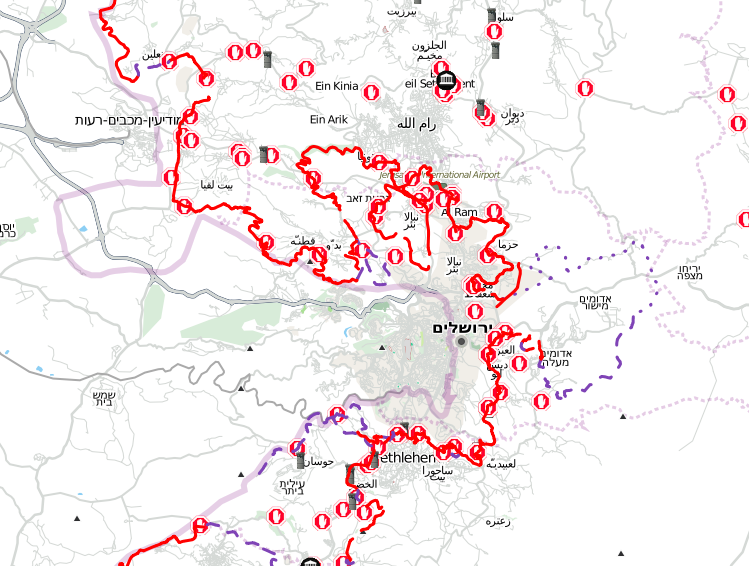
\includegraphics[width=0.45\textwidth]{images/levinger-groundtruth.png}
		\caption{The Green Line, Israeli settlements, and checkpoints near Jerusalem and Ramallah, on Josh Levinger's GroundTruth interactive map. (\url{http://groundtruth.media.mit.edu})}
	\end{flushright}
\end{wrapfigure}

VirtualGaza, a project by Josh Levinger, published narratives by victims of the 2008 war in Gaza, linking the cartographic representation(one reason for the conflict) with the human stories and images it caused. The OpenLayers-based map, available at \url{http://virtualgaza.media.mit.edu}, protected participants' locations by purposely categorizing them by region instead of displaying more precise coordinates. Levinger's second project in the area, GroundTruth, demonstrated a routing algorithm which could, given a user's legal status, create a travel plan which would avoid IDF checkpoints, actively seeking to disrupt the balance of power in the region by using cartographic information.\footnote{The routing system was disabled when it became clear that up-to-date checkpoint information was unavailable, and that users might be presented with obsolete data.} Other cartographers have during the same conflict in Gaza, Mikel Maron defended his work towards the participatory creation of a free and open map of Gaza:  

\begin{quote}
...it's frankly the same security through obscurity argument peddled for centuries... a strategy on the verge of finally dissolving in a world of openness and transparency. The IDF access to much better intelligence and imagery than we'd ever have, they fly drones over Gaza, there's a 2m resolution commercial limit in all satellite imagery over Israel — guess who gets to see the sub-meter imagery? Gazans have nothing to gain by trying keep secrets, the asymmetry of that game is overwhelmingly not in their favor. \cite{maron2009misconceptions}
\end{quote}

Maron later refined his position to except certain highly vulnerable groups \footnote{See Section \ref{sec:ethics} for a discussion of PGIS ethics}:

\begin{quote}
In general, I view these edge cases as a question of power. Hiding information protects those already in power, but not those that are already marginalized. Legitimate cases to me is only information that puts dis-empowered people at risk, such as refugee routes along the Burmese-Indian border. \cite{maron2010freedom}
\end{quote}

However the gist of his argument is sound --- that cartography is necessarily a losing game only for those who are unable to participate in its creation. Those who are unable to communicate in the relevant cartographic language of power -- be it GeoJSON, \ac{TMS} or just paper -- never even know they are being mapped, or what that might mean for their well being or safety.\footnote{A common criticism by PGIS practitioners of so-called `remote sensing'. See Section \ref{subsec:pgis}} In some ways, this is a subset of the debate championed by Evgeny Morozov, Clay Shirky, and Patrick Meier\footnote{See \url{http://www.prospectmagazine.co.uk/2009/11/how-dictators-watch-us-on-the-web/} for the Morozov/Shirky debate, and \url{http://irevolution.wordpress.com/2010/01/07/morozov-vs-shirky/} for Patrick Meier's analysis.} over whether new media is a force for democracy, or at least whether it supports `popular resistance against repressive rule' as Meier puts it. \cite{meier2010popular} Morozov even mentions mapping repeatedly, for example when he ridicules the sappiest anecdotes of the technological freedom fighters: 
 
\begin{quote}
...Burmese monks defying an evil junta with digital cameras; Filipino teenagers using SMS to create a “textual revolution;” Egyptian activists using encryption to hide from the all-seeing-eye of the Mukhabarat; even Brazilian ecologists using Google maps to show deforestation in the Amazon delta. \cite{morozov2009dictators}
\end{quote}

In Morozov's opinion, the belief that such technologies can disrupt power relations `...requires certainty that only pro-western and pro-democracy forces will participate.' His examples, though anecdotal, are sobering: `In Russia, the internet has given a boost to extreme right-wing groups like the Movement Against Illegal Immigration, which has been using Google Maps to visualise the location of ethnic minorities in Russian cities and encouraging its members to hound them out.' 

(rev. see following quote)

The problem with this debate is that it is too abstract. We cannot say universally that map-making (or any other technology) will support local needs over those of the state, but by working closely with local participants in a sensitive manner, we can invert the flow of information and affect power relations. Balloon and kite mapping is not a scalable technology --- it would be impractical for Google or governments to use these techniques to map entire countries. However it is well adapted for small-scale use, and has important advantages in cost, repeatability, resolution, and speed, in that context. My attempts to apply these tools and techniques have focused on these benefits, and in the specific settings in which I have worked, they have allowed local groups to produce better maps than anyone else, for a limited but \textbf{highly relevant} area. In a time when many in the crisis community were struggling to get large organizations such as Google, the United Nations, etc. to release satellite imagery\footnote{See Section \ref{subsec:satelliterelease}}, the Louisiana Bucket Brigade actually licensed map data to Google -- data gathered using Grassroots Mapping tools and techniques.\footnote{See Chapter \ref{chap:gulf}} 

(more to do with adoption, appropriation - hence focus on collaboration, pedagogy, by and with local groups, rather than boolean)

\begin{quote}
Research on the Internet’s role in politics has struggled to transcend technological determinism—the assumption, often inadvertent, that the technology simply imprints its own logic on social relationships. An alternative approach traces the ways, often numerous, in which an institution’s participants appropriate the technology in the service of goals, strategies, and relationships that the institution has already organized. --- Agre, Philip E. 2002. “Real-Time Politics: The Internet and the Political Process.” The Information Society 18:311-331.
\end{quote}

`Technology only magnifies human intent and capacity. It cannot substitute for them' --- Kentaro Toyama

Corbett, Jon M., and C. Peter Keller. 2005. An Analytical Framework to Examine Empowerment Associated with Participatory Geographic Information Systems (PGIS). Cartographica 40 (4):91-102.

\section{Maps as truth}
\label{sec:truth}

\begin{wrapfigure}{r}{0.5\textwidth}
	\begin{flushright}
		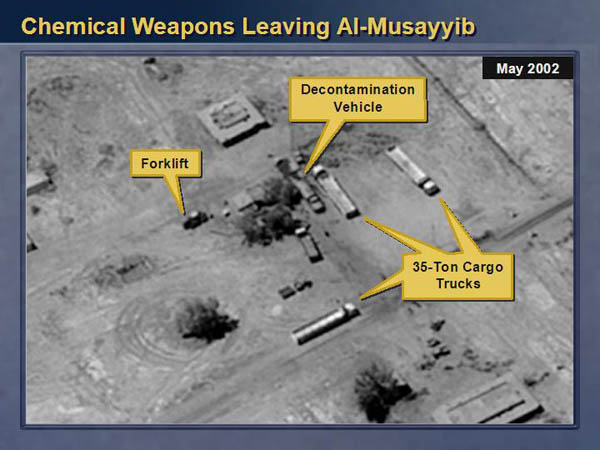
\includegraphics[width=0.45\textwidth]{images/iraq-image-16.jpg}
		\caption{\url{http://www.gwu.edu/~nsarchiv/NSAEBB/NSAEBB88/}, Image 16: Chemical weapons leaving Al-Musayyib}
	\end{flushright}
\end{wrapfigure}

Maps carry a sense of authority that few other forms of evidence share. This is in part due to an understanding of satellite or aerial maps as a kind of `window into the world', depicting the planet `the way it really looks'. In photography, by contrast, the editorial and subjective role of the author is accepted, despite the damage which `photoshopping' has inflicted on the perceived truth or objectivity of the photographic image. Maps, however, continue to be taken as direct representations of reality, desipte the inherent subjectivity of image selection, color, brightness, and contrast processing, and the editorial eye necessary in reading and interpreting such imagery. 

The best example of this attitude is of course the use of relatively poor resolution satellite imagery by Colin Powell at the UN Security Council in February 2003, which he presented as evidence to support the existence of weapons of mass destruction in Iraq. While the subsequent complete absence of weapons did little to diminish the public's faith in such imagery as objective evidence, Powell mentions in his testimony how difficult it is to interpret satellite imagery:  

% citation http://www.un.org/apps/news/storyAr.asp?NewsID=6079&Cr=iraq&Cr1=inspect

\begin{quote}
Let me say a word about satellite images before I show a couple. The photos that I am about to show you are sometimes hard for the average person to interpret, hard for me. The painstaking work of photo analysis takes experts with years and years of experience, pouring for hours and hours over light tables. But as I show you these images, I will try to capture and explain what they mean, what they indicate to our imagery specialists.

...

How do I know that? How can I say that? Let me give you a closer look. Look at the image on the left. On the left is a close-up of one of the four chemical bunkers. The two arrows indicate the presence of sure signs that the bunkers are storing chemical munitions. The arrow at the top that says security points to a facility that is the signature item for this kind of bunker. Inside that facility are special guards and special equipment to monitor any leakage that might come out of the bunker.

The truck you also see is a signature item. It's a decontamination vehicle in case something goes wrong.
\cite{guardian2003powell}
\end{quote}

Despite the `years and years of experience' he claimed, an earlier analysis of the imagery to which Powell had access classified the claims as `weak' and points out that the so-called contamination vehicles are in fact simply water trucks. Though they acknowledge that these \textbf{could} have been used for chemical weapon decontamination, the doubt they express stands in contrast to the assertion of `facts' that Powell presented to the UN: 

\begin{wrapfigure}{r}{0.5\textwidth}
	\begin{flushright}
		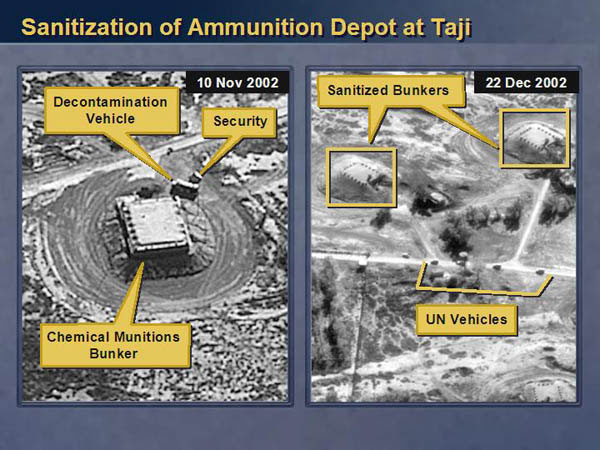
\includegraphics[width=0.45\textwidth]{images/iraq-image-13.jpg}
		\url{http://www.gwu.edu/~nsarchiv/NSAEBB/NSAEBB88/}, Image 13: Sanitization of Ammunition Dump at Tajii	
	\end{flushright}
\end{wrapfigure}

\begin{quote}
	``--- 10-11.***/WEAK. We support much of this discussion, but we note that decontamination vehicles--cited several times in the text--are water trucks that can have legitimate uses. A safer characterization is, `a vehicle used for chemical weapon decontamination.`

--- 11.***/WEAK. We agree there has been suspicious activity [redacted], including presence of a decontamination vehicle. We caution, however, that Iraq has given UNMOVIC what may be a plausible account for this activity--that this was an exercise involving the movement of conventional explosives; presence of a fire safety truck (water truck, which could also be used as a decontamination vehicle) is common in such an event."
	October, 2002, classified National Intelligence Estimate (NIE) `Iraq's Continuing Programs for Weapons of Mass Destruction' \cite{senate2004report}
\end{quote} 

What is most alarming about this kind of rhetorical use of map imagery is that it represents a means for those in a position of power to assert or twist truths about places they have never been, without the involvement of human testimony from those who have. The public perception of maps as an objective, quantitative standard of evidence is likely due to the difficulty and expense of producing map imagery, and the traditional monopoly of government and high-tech industry in the production of such imagery. Still, as we see in Powell's testimony, clearly even the highest levels of government are complicit in the construction of maps as an authoritative and objective form of information.

\section{Maps: rhetorical, even tactical}

This use of mapping as a form of political persuasion is nothing new, from a historical perspective, but the increased couching of such information in technical terminology and the use of exact measures --- referring to maps by their `centimeter accuracy', for example --- has made it more difficult for lay persons to critique. As Dennis Wood points out in his classic `The Power of Maps', such metrics give the `false impression of ``scientific accuracy'' and completeness'.\footnote{Wood, p.20-21}

(More on social construction of maps, Dennis Wood quotes... get reference on return to Boston)

%        - Endless variety of possible data: Wood, Power of Maps, p.1
%        - not a representation of truth, but a rhetorical tool; Wood, p1?
%            - social construction of maps
% 	- map of sewer system from Wood

(Order new copy of Radical Cartography, get refs for next section)

It is this rhetorical aspect of mapping which the Institute for Applied Autonomy explores, along with `Tactical cartography', in their essay of that name. By not only fighting a war of words (or pictures) in highlighting issues of concern, but producing maps which act as tools in the direct intervention in problematic situations, a transition is made from the important discursive products of maps-as-information to their use as informational weapons in a direct engagement. In this vein, the Institute authored a pocket map in 200x depicting all surveillance cameras in Manhattan, so that users might not only learn about the increasing prevalence of a surveillance society, but actively avoid zones under surveillance in their daily life. This move beyond a symbolic role for mapping --- to legal, activist, and primarily action-based outcomes, is what I have attempted to engender in the Grassroots Mapping project.

\section{Cartographic ethics}
\label{sec:ethics}

In light of this reassessment of the political and social roles of maps and their production, some from the PGIS community have called for a code of ethics in participatory mapping projects. This seems especially prudent given that the production of maps can have dramatic effects on the residents of the mapped area. Giacomo Rambaldi, Robert Chambers, Mike McCall, and Jefferson Fox proposed in 2006 a set of 33 guidelines entitled `Practical ethics for PGIS practitioners, facilitators, technology intermediaries and researchers'. The following is a sampling:

\begin{quote}\begin{itemize}
\item Do your best to recognise that you are working with socially differentiated communities and that your presence will not be politically neutral
\item Consider using spatial information technologies that can be mastered by local people (or local technology intermediaries) after being provided sufficient training
\item Be considerate in taking peoples' time
\item Stimulate spatial learning and information generation rather than mere data extraction for outsider’s analysis and interpretation
\item Ensure that the outputs of the mapping process are understood by all those concerned
\end{itemize}
\cite{rambaldi2006practical}
\end{quote}

These guidelines demonstrate an belief that maps should be produced \textbf{in collaboration with} local communities, and with respect for their needs and interests. Even in the context of an openly activist agenda, they have proved invaluable to me in formalizing and understanding his interactions with mapping participants. In particular, they address the core concern of who owns the maps and for whom they are made; there is often the implicit assumption by enthusiasts of open geodata that simply dumping map data into OpenStreetMap is the end goal. It is important to be aware that most people (and especially those in communities in geographic conflict) are unaware of the existence of OpenStreetMap, and would likely be unreceptive to its benefits. 

Robert Chambers in particular warns PGIS practitioners against raising expectations of concrete results, noting that `Any process of analysis facilitated by an outsider is liable to raise expectations of some benefit, even when the outsider goes to pains to explain that they have nothing to offer and nothing will follow from their visit. Disappointment, and reinforced disillusion with visitors and organisations outside the community then follow.' \cite{chambers2006whose}

(email exchange from PPGIS list from early June) 

\chapter{The Need for Geospatial Data}
\label{chap:need}
\section{Two worlds of mapping}
\label{sec:twoworlds}

Present-day users of web-based mapping products such as Google Maps are presented with an extremely rich cartographic landscape when they view maps of first-world urban centers such as New York and San Francisco. Real-time traffic data is often overlaid in lines of shifting red and green, and many buildings appear in orthographic '3D'. Well-known restaurants are interspersed with subway stops whose schedules may be called up with a few clicks. Routing algorithms offer turn-by-turn directions, optimized for pedestrians, bicyclists, and motorists. 

\begin{figure}[h]
	\begin{center}
		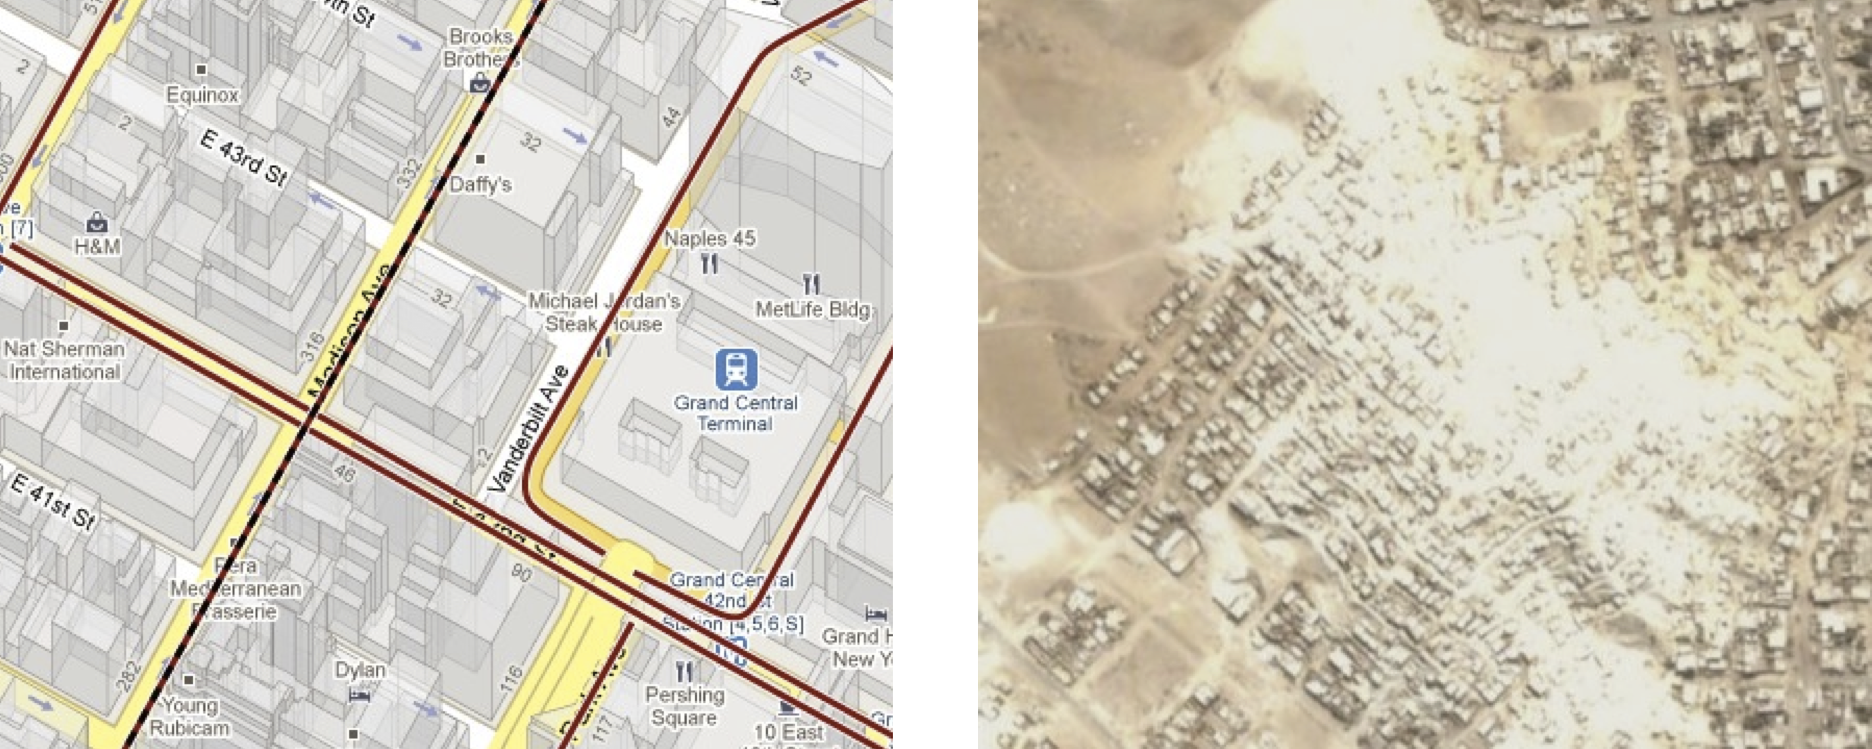
\includegraphics[width=1\textwidth]{images/two-worlds-mapping.png}
		\caption{Views of Manhattan, left, and a settlement in Lima, Peru, right, as seen in Google Maps \url{http://maps.google.com}}
		% could add Cameroon, where towns are missing
	\end{center}
\end{figure}

Many are surprised when they view places such as Lima, Peru, a metropolis of 11 million people, and find that not far from the city center are vast areas of indistinct and unlabelled buildings. While some of these are recognized and official parts of the Municipality of Lima, many are informal settlements, whose inhabitants lack title to their plots of land, and whose streets and buildings do not appear on any city map. Many of these settlements, or `invasions' as they are known to Peruvians, are governed by leaders who are either elected by the several hundred inhabitants, or who maintain control through intimidation --- employing thugs to collect taxes and enforce rules. 

This state of extralegal urban sprawl exists in many parts of the world, and according to UN-HABITAT, up to a quarter of the world's population lives in similar conditions.\footnote{Cite UN-HABITAT} A legal process may exist to establish official land ownership in these settlements, and to issue deeds to their inhabitants (as it does in Peru), but in many cases the state lacks the resources to quantify or map these areas:

(Quotation on `lack the means to ...' --- UN-HABITAT)

While accessible and participatory map-making is by no means a solution to this problem, many of the negotiations occurring in such areas are taking place in the language of cartography --- whether intentional or not, cartographic invisibility is often the first step to settlements' exclusion from planning processes: 

\begin{quote}
...slums - all variety of precarious settlements - represent the `invisible' city, often omitted from official maps and documents and frequently physically hidden by local authorities by colorful walls and fences. 
--- `Slums of the World', UN-HABITAT, 2003 \cite{}
\end{quote}

(Map of highway over a slum, Jai Sen, blank map of favelas in Rio chosen as Olympic sites, Kate Balug)

`geographical mapping techniques to support struggles for social justice in India'. The end result, it added, could make maps as `tools to fight injustice in society'.
--- \url{http://timeoutbengaluru.net/aroundtown/aroundtown_feature_details.asp?code=59}

The Grassroots Mapping project was conceived as a means to broaden access to mapping technology, and was developed in direct response to the need for maps in informal settlements on the outskirts of Lima, Peru.

PGIS researchers have also established a strong case for the diverse uses of participatory maps. Robert Chambers lists several, ranging from benefits to outside aid organizations to direct benefits to the local community, including:

\begin{quote}
\begin{itemize}
	\item{`Social mapping, identifying people 5, livestock, children who do and do not go to school, people in different livelihood and other social categories, wealth and wellbeing groups...}
	\item{`Health mapping, for people with health problems, disabilities, special knowledge etc in communities. In the UK participatory mapping by women has shown the location and concentrations of breast cancer (Lynn et al n.d.)}
	\item{`Farm mapping, combined with mapping of nutrient flows within the farm and over the farm boundaries (as undertaken by many organic farmers in Karatina, Nyeri District, Kenya in 1996)'}
\end{itemize}
\cite{chambers2006whose}
\end{quote}

\section{Environmental assessment}

As Chambers notes, beyond issues of land rights and ownership, there are many other potential uses for inexpensive map data; the ability to produce photographic, or raster maps of sensitive environmental sites may empower small organizations which are unable to acquire timely or high resoultion satellite images of sites of interest. Aerial imaging is a form of map-making particularly suited to environmental monitoring due to its ability to not only delineate regions of social and political interest, but raster data which can be used to compare plant growth, erosion, and even animal life. One case study we will examine is that of a group of environmental activists known as Coal River Mountain Watch. The West Virginia-based group have sought to gather meaningful and quantitative evidence of the environmental damage and health hazards of mountaintop removal mining across the Appalachia region of the United States. Besides the prohibitive cost of traditional satellite imagery and high level of expertise required by traditional GIS tools, they and other environmental activists strive for data which will make a visceral and emotional impact on policymakers and regulators, as well as the general public. 

Currently, activists in Appalachia make widespread use of water conductivity tests to determine the degree of contamination in waterways due to runoff and blackwater releases. Conductivity is a secondary measure, and, though highly standardized, cannot convey the same sense of urgency as photography of, for example, a blackwater release, or the devastation that persists even in supposedly replanted reclamation sites. Aerial imaging, or specifically mapping, is an ideal blend of direct measurement and visual impact, and its main detractor is its price; overflights cost hundreds or thousands of dollars each and image processing is labor- and skills-intensive. A collaborative project examining the applicability of Grassroots Mapping tools to this problem was performed in May 2010 and is discussed in Section \ref{sec:ongoinguses}.

\subsection{Asset allocation mapping}

Asserting a voice in the management of natural resources is dependent on quantitative information on the extent and valuation of the land, which is often carried out using GIS, a language of power from which local communities are often completely excluded. Peter Poole's article `Is there Life after Tenure Mapping?' and report `Information: the First Conservation Asset' examine in detail a number of case studies where participatory mapping was used by indigenous communities to support the `stewardship of biodiversity' \cite{poole2007belize}. Citing examples of his and others' work from Venezuela, Suriname, Belize, and elsewhere, Poole shows how cartographic techniques were used not only to monitor the activities of industrial development and extraction industries, but in some cases to take legal action against such initiatives.  

Poole distinguishes between asset-based strategies and rights-based strategies, where the former seeks to assert local control over territory in specific actions against asset extraction industries, rather than the rights-based approach of seeking broad legal recognition of territorial claims at the state level. \cite{poole2006there} While some of the examples he cites make use of GPS track collection or sketch mapping, this emphasis on assets often necessitates raster imagery instead of coordinate data, and as such, Poole's project in Belize has made use of light aircraft photography, as well as kite and balloon photography, in collecting and presenting evidence to support claims. \cite{poole2007belize} The successes of this strategy present an exciting opportunity for such dramatically lower cost aerial photography techniques as offered by the Grassroots Mapping project, and I am excited by the prospect for future collaboration.

\section{Open geodata and crisis mapping}
\subsection{Crisis mapping and Ushahidi}

The ability of participatory mapping to provide maps on-demand has obvious applications in disaster response and management. A variety of different crowdsourced or grassroots mapping strategies have evolved in recent years with the intent to respond to, document, analyze, and report on the real-time occurrence of disasters and crises. From environmental crises such as the April 2010 BP Oil Spill in the Gulf of Mexico to the humanitarian crisis in the aftermath of the January 2010 Haitian earthquake, a clear need has evolved for low-cost, decentralized situational awareness and documentation tools with geospatial features. Here we discuss some of the challenges of fulfilling such diverse needs under unpredictable conditions.

\subsubsection{Ushahidi}

The Ushahidi platform has emerged as a common and easy-to-install system for crowdsourced crisis reporting. Developed in collaboration with Kenyan programmers to help voters report election violence in Kenya in 200x, it allows citizens with mobile phones to send 140 character text messages to a publicized telephone number. \cite{okolloh2009ushahidi} These messages are read by a group of editors, who attempt to identify where the messages were sent from, and are published on a web site as red dots at their assumed location. That users self-report their locations, and can do so incorrectly, is tolerated because it may represent a means of privacy for some users, and because in the aggregate it is quite difficult to `fake' an event. (cite Meier's post) Each report is verified if possible by ..., however in many cases no verification is possible, yet in emergency response situations this has proven not to impede the use of Ushahidi data by agencies such as (in the Haitian earthquake of January 2010) the Coast Guard, the US Marine Corps, and FEMA. \cite{meier2010crowdsorcerors}\cite{meier2010ushahidi} 

% interview LABB folks about how reports are verified

Ushahidi works in many cases because it is simple to understand on its surface: visitors to an Ushahidi web site see a series of dots with messages such as `I'm stuck under rubble' and imagine a person sending such a message from their cell phone. It makes use of existing communications infrastructure, namely that most people have cell phones and relies on both a high level of literacy with text messaging and a willingness to send reports to a site which is not immediately viewable. However, it is not a means to `make' a map per se, but rather to collect data on events occurring at specific times, and correlating them with an existing map.

Ushahidi has been successfully used to gather and publish extremely up-to-date information about unfolding crises, for example in the instance created by the New Orleans-based environmental group \ac{LABB} in response to the BP oil spill in April 2010. The kind of information it provides, however, is difficult to verify or to quantify, and is more useful in the context of emergency response than in evidence-gathering. \cite{meier2010verification} Locations must often be approximated to the nearest town or city, and most reports are often just a few words with no name or photographic evidence. While geotagged photographs can be uploaded to Ushahidi, EXIF data can be falsified. In many cases there is an additional need for quantitative data. Map imagery provides more comprehensive information in that every pixel of a map has a corresponding location in the real world, allowing it to be correlated against other maps. 

However, a combined strategy involving the use of an Ushahidi-like platform with aerial imaging can result in clusters of crowdsourced reports providing target sites for followup map-making sessions. This process was employed in the BP oil spill in the Gulf of Mexico between the \ac{LABB} Ushahidi instance and \ac{LABB}-led Grassroots Mapping trips.\footnote{See Chapter \ref{chap:gulf}} Maps of oil-affected areas were then posted back to the Ushahidi site as \ac{TMS} layers.

%\subsubsection{Photographs and maps as testimony}

\subsubsection{Satellite imagery}
\label{subsec:satelliterelease}

Public access to up-to-date imagery of crisis areas has become something of a hot-button issue in crisis mapping circles, as those companies and agencies in control of the imagery do not always elect to release it, or to license it freely for any use. Whethe due to an unwillingness to offer expensive imagery for unrestricted use, or due to the administrative burden of actually offering such data for download under a permissive license, access to satellite imagery has become a frequent bottleneck for aid organizations. 

Specifically in the bottom-up response to the Haitian earthquake and subsequent humanitarian crisis of January 2010, access became more difficult within weeks of the crisis. While GeoEye and other vendors generously offered open access to satellite imagery in the initial weeks of the crisis, most did not elect to do so on an ongoing basis, or for subsequent crises such as the February 2010 earthquake in Chile. This has caused a great deal of frustration for those outside the largest and wealthiest organizations. Specifically, Google and GeoEye's decision to revert to their standard license for new satellite imagery of Port au Prince after January 2010 elicited questions from the broader crisis response community, as voiced by Mikel Maron on the Crisis Mappers mailing list in late April 2010:

\begin{quote}
Maybe you can explain why Google has not continued the extremely helpful position it had in January?
Is the community of CrisisMappers doomed to lose that culture of sharing? Can't we do better?
\end{quote}

In the February 2010 earthquake in Chile, a similar plea for imagery was sent to the same list, prompting a reply from a UN-SPIDER representative. UN-SPIDER or the United Nations Platform for Space-based Information for Disaster Management and Emergency Response, is an organization whose self-described aim is in `providing universal access to all types of space-based information and services relevant to disaster management' which it fulfills by `serving as a bridge to connect the disaster management and space communities...' \cite{unspider2010aims}. However, the organization has been slow to adopt truly open data sharing policies, and to date makes relatively few data sets available to the public; most are reserved for Authorized Users --- typically government agencies and large disaster response organizations. \cite{charter2010brochure}  

Ultimately, citizen-led mapping efforts present an opportunity to bypass this bottleneck by providing high-resolution, timely aerial imagery at low cost. Such an effort occurred during and after the 2010 BP oil spill in the Gulf of Mexico and is discussed at length in Chapter \ref{chap:gulf} 

(Cite Remote Sensing table)

% who released data??? 

\chapter{State of the Art}

\subsection{Participatory GIS for Development}
\label{subsec:pgis}

Traditional GIS technology has been used for since the 1990's to support communities in developing contexts for purposes such as making tenure claims, environmental defense against petroleum and other extraction industries, as well as for planning purposes. This has become known as PGIS, or Participatory GIS, and typically... 

% See Peter Poole's Life after Tenure Mapping for a brief historical timeline, i think

`how GIS, spatial data, and maps produce and negotiate politics and power relations, or how they can be used to foster participatory decision making processes.' -  bibliography/rambaldi-participatory-spatial-developing-countries.pdf

% Jen Osha's article
%\href{http://www.directionsmag.com/article.php?article_id=2365&trv=1.}{Participatory GIS - A Paradigm Shift in Development?} - Jen Osha and Daniel Weiner, 2006

\href{http://www.directionsmag.com/article.php?article_id=2365&trv=1.}{Participatory GIS - A Paradigm Shift in Development?} - Jen Osha and Daniel Weiner, 2006

Sarah Elwood summarizes various alternative GIS movements, one which ``could incorporate diverse forms of spatial knowledge and promote multiple epistomologies" \cite{elwood2009representations}

%        THE ILLUSTRATED GUIDE TO NONPROFIT GIS AND ONLINE MAPPING: http://maptogether.org/nonprofit-mapping
%        Claudia Canepa's PhD dissertation
\subsection{Challenges of conventional PGIS practice}
\label{subsec:pgisshortcomings}

Critics of PGIS practice point out that despite the emphasis on inclusion in the map-making process, final map processing is often outsourced

More to the point, there persists a detached anthropologic attitude wherein PGIS researchers are `capturing' data; there is a definite note of surprise that `indigenous' communities, whether in sub-Saharan Africa or simply in communities without a high degree of technical fluency, could author good maps. The excitement over the moment of cartographic understanding which the following quotation depicts is tempered by the condescension it suggests: 

\begin{quote}
It was also in 1988 in an AKRSP (India) RRA training... that a headman, asked to present to the villagers the map the outsiders had draw, had difficulty until he turned it ``upside down", which was the way he and the villagers saw their village . . . . We were teetering on the brink of learning that ``They can do it".
\cite{chambers2006participatory}
\end{quote}

PGIS researchers have not been insensitive to these issues; Robert Chambers...  `Many ethical issues present troubling dilemmas, and lead to overarching questions about empowerment and ownership. Questions to be asked, again and again, are: Who is empowered and who disempowered? And, who gains and who loses?' \cite{chambers2006whose}

In practice, there is a question of formats: while for many communities a paper map would be the ideal end product, many cartographers feeel the need to produce digital maps in a variety of formats, such as shapefile, KML, WMS, etc. This raises the question of who the intended audience is --- the funding agency, perhaps, or the PGIS academic community, or even the blogosphere. These are valid considerations; if the map-making is intended to help a community to communicate with official entities, i.e. to affect a cartographic power relation, a digital end product may help to `translate' local knowledge into the relevant language of power. 

As a result, many PGIS map projects outsource the final processing of map data to GIS experts. While in many cases this may seem like the only way to produce a completed map without the time and expenditure of training local participants in the use of GIS software, perhaps starting with basic computing skills, it may also be a means to build a better and more integrated relationship between the local community and those governmental entities they are attempting to communicate with. However, this is speculative and Peter Poole writes that such an advantage `has yet to be widely demonstrated', citing examples in Suriname and Venezuela. He further points out that outsourcing ties local communities to the expert GIS entity in the event that they wish to repeat or extend their mapping efforts. \cite{poole2006there}

Beyond these pragmatic difficulties presented by outsourcing,  

\section{Web mapping}
\label{sec:webmapping}
Some degree of mapmaking ability has become commonplace to the internet-connected public since the advent of highly user-friendly `slippy map' interfaces such as Google Maps. This has been especially true since the release of the Google Maps Application Programmer's Interface (API) in the summer of 2004, allowing programmers to modify and repurpose Google's web map services.  Early examples of reuse included the GMaps Pedometer, which would output the linear distance of a path you walked, along with how many calories you burnt. \cite{gibson2006google} From the frivolous to the essential, this means of mapmaking has become widespread and relatively easy. However, many would argue that this is not mapmaking at all; most of the users of Google maps do not edit the underlying map data, but overlay points, lines, and polygons \textbf{on top of} Google's proprietary data.

\subsection{Google Maps and proprietary data}

In fact, not only Google Maps, but the vast majority of the online maps are based on the relatively static base maps made available by larger organizations. Google and other providers of map data publish these maps as collections of small image 'tiles'; JPG or PNG images of typically 256 by 256 pixels, which are rendered ahead of time and cached. These are served using Apache or another conventional web server. The main benefit of this technique is that it serves map data as a set of common image files; a standard and highly optimized means of distribution. These are re-assembled in the browser into a seemingly continuous map, and as the user pans or `slips' around, new tiles are transferred to maintain the illusion of a continous map.

A second reason for the use of map tiles is that it is quite difficult to reconstruct the original discrete vector data set from map tiles; in this respect they are similar to compiled code. Google and other commercial map vendors do not share their point, line, and polygon data, nor do they make metadata such as labels or land use markers available. Distributing tiles gives them a degree of control over what source data they choose to release, and allows them to maintain control of those assets.

Distributing the underlying data used to generate these tiles conflicts with these companies' business models: such data is valued intellectual property. The tile-based rendering system strips the map of its metadata, making a local, or personal, critical, or revisionist interpretation quite difficult. Tiles immutable – they contain no information about authorship, no hyperlinks, and in order not to crowd a given tile, each one displays only a selection of available data for that corresponding area of the world. 

\begin{wrapfigure}{r}{0.5\textwidth}
	\begin{flushleft}
		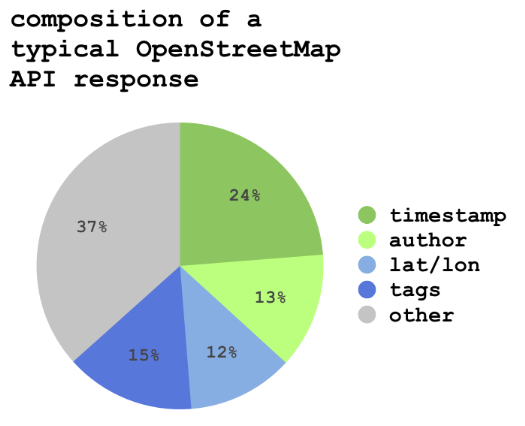
\includegraphics[width=0.45\textwidth]{images/osm-composition.png}
	\end{flushleft}
\end{wrapfigure}

Open data projects such as OpenStreetMap, the 'wiki map of the world', do just the opposite – like the open source software projects they took inspiration from, they share the entire dataset as coordinates, semantic tags, polygons, and most importantly, time and authorship data. In the case of OpenStreetMap, anyone with enough disk space can download the entire planet's worth of data (over 200 gigabytes when loaded into a database) and create their own maps. In that dataset in particular, authorship data actually outweighs its geometric counterpart. Perhaps even more tellingly, historical data – for areas of the map which have been overwritten – occupies more storage space than current data. This suggests that authors have challenged each others' data more than they've added new data to unmapped areas. \cite{warren2009composition}

\section{OpenStreetMap}
\label{sec:openstreetmap}

OpenStreetMap.org, taken as an open-source software project, a database of open geodata, and a community of volunteer mappers, represents one of the best examples in recent years of the \textbf{neogeographic} response to PGIS. That is, without explicit ties to the PGIS movement, or reference to the movement's two decades of literature and research, OpenStreetMap (or OSM, as it has become known in neogeographic circles) has attempted to meet many of the same goals since its founding in 2004. OSM encourages volunteers around the world to contribute to a single, shared digital map and corresponding map database. \cite{chilton-crowdsourcing} 

In many ways it has met with wild success, and the size and detail of the OSM map database is formidable. In July 2010, the project included over 700 million points, making up some 56 million polygons, all contributed by more than 280,000 users. \cite{osm2010stats} However, participants are overwhelmingly European and American, and tend to be wealthy due to the emphasis on internet connectivity and the use of GPS devices to produce new map data.

In fact, the OSM data collection strategy relies most heavily upon three sources. First, existing municipal and public domain databases make up an enormous part of the available data; the TIGER database produced by the US Census increased the size of OSM by a factor of twenty. \cite{willis2007osm} Second, tracing of satellite data with the Potlatch, JOSM, and other tools to extract vector data from rasters plays a large role, especially in areas with few local participants. This technique was used in the OSM Gaza project to map all of Gaza using a satellite dataset purchased for \$5,000 from DigitalGlobe using donations during the Gaza war in late 2008. \cite{maron2010openstreetmap}\cite{chilton-crowdsourcing} While convenient in that it does not require mappers to actually travel to the places they are mapping, it does not actively involve residents of an area in the mapping process, and sufferes from many of the shortcomings which inspired the PGIS movement. 

Finally, much of the OSM database was created by individuals carrying GPS devices to record GPX tracks, or collections of latitude/longitude coordinates. These are later uploaded, annotated and merged into the main OSM database using tools such as JOSM. This is the preferred means of collecting data because of its high accuracy, its emphasis on firsthand mapping, the clear legal ownership of the data, and because of the implicit belief among many OSM participants that better maps are made `on the ground'. 

This belief is supported by the `on the ground' policy stated explicitly in the OpenStreetMap wiki, a central organizing document of the community.

\begin{figure}[h]
  \begin{center}
    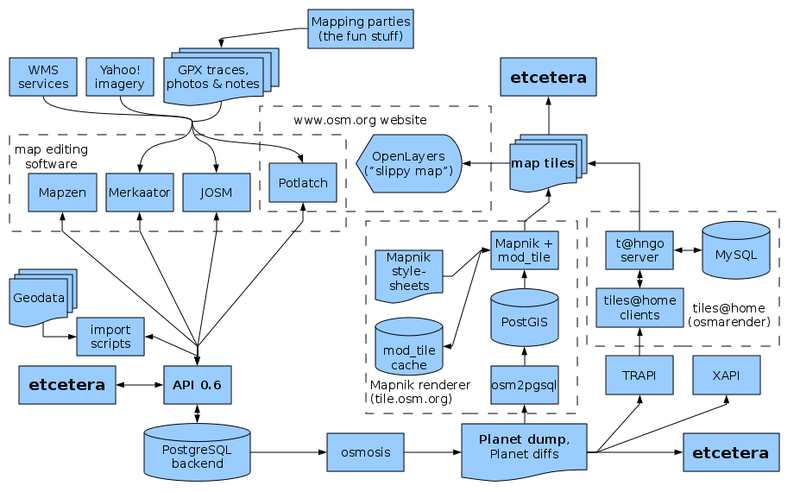
\includegraphics[scale=0.45]{images/osm-diagram.png}
  \end{center}
\end{figure}

\subsection{The modern open-source geostack}

Another interesting aspect of OpenStreetMap is that it represents a deployed and working combination of many of the premier open-source mapping tools available today. It makes use of OpenLayers, a web browser-based framework for displaying raster map tiles using JavaScript. Tiles are produced using Mapnik, the popular open-source tile renderer. An array of other open-source utilities are used to create, edit, translate, import, and export the data. The Grassroots Mapping project, and especially the Cartagen Knitter, can be seen as an opportunity to augment this geostack with an equally open means of capturing source imagery and integrating such data into the open-source workflow. 

\subsection{Humanitarian OSM Team}
 
An offshoot of the OpenStreetMap project known as the OpenStreetMap Humanitarian Team or HOT was started in late 2009 by Mikel Maron, a map programmer and co-founder of mapping firm Mapufacture. Positioned in direct response to the need for maps in areas of humanitarian crisis, Mikel has organized members from the technology community to visit crisis zones such as Port-au-Prince as well as a long-term presence in Kibera, a large slum in Nairobi, Kenya. HOT uses the same tools as the wider OpenStreetMap community, and either runs a separate instance of the OpenStreetMap server and database, or directly uploads the data to the main OpenStreetMap.org service. 

\url{http://wiki.openstreetmap.org/wiki/Humanitarian_OSM_Team}

\subsubsection{OSM Gaza}

HOT's first project, a volunteer effort to map the Gaza Strip during the 2008-2009 war between Israel and Gaza, relied on Yahoo Maps and Digital Globe satellite imagery. Over seven days, OpenStreetMap volunteers traced the satellite imagery in order to produce a more accurate, more up-to-date map, and with assistance from JumpStart International, the map was available online and for download with no copyright restrictions. \cite{chilton-crowdsourcing} This emphasis on placing map data (not just rendered maps!) in the public domain was intended to provide for the widest possible uses of the information, on both a technical and legal basis. In order to preserve this legal status, the OSM Gaza dataset was published separately from the main OpenStreetMap database, though in accordance with its liberal licensing, a copy was uploaded to OSM as well. Building on the success of the OSM Gaza project, HOT went on to collaborate with a variety of organizations in countries like India, Kenya, and Georgia, all using the OpenStreetMap toolset. 

\begin{figure}[h]
  \begin{center}
    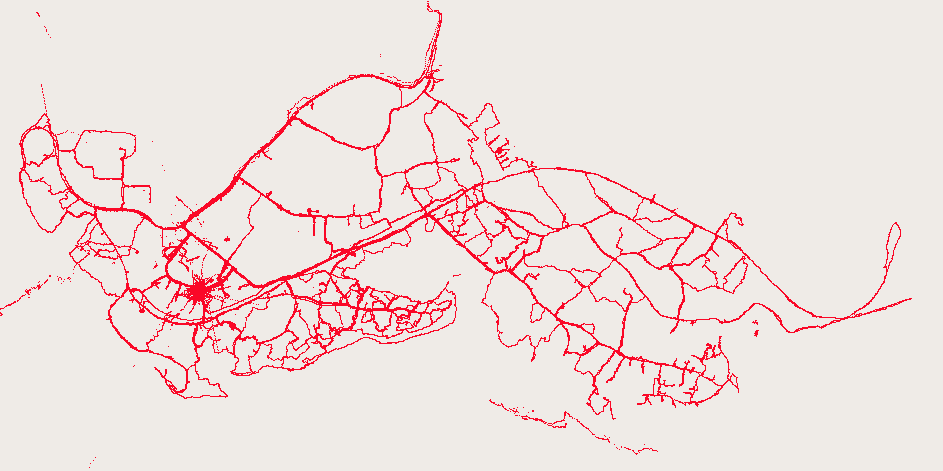
\includegraphics[width=1\textwidth]{images/kibera-gpx.png}
    \caption{GPX traces collected from GPS units over three weeks of mapping in Kibera. \url{http://www.flickr.com/photos/mikel_maron/4143021346/}}
  \end{center}
\end{figure}

Two projects by HOT stand out as their most ambitious and influential. The first, called simply Map Kibera, produced a map of the famous Kibera slum in Nairobi, Kenya, in collaboration with several local organizations. This project differed from earlier HOT projects in that it relied primarily upon local participants using hand-held GPS units to produce the map, as well as with paper-based annotations using the Walking Papers system developed by Michal Migurski of Stamen Design. With a specific mission to engage with the sociopolitical aspects of cartography, Map Kibera is much more explicit than OSM Gaza in its agenda and the needs it addressed. It also represented a shift away from remote mapping by means of tracing, towards a model which relied more heavily on local expertise and familiarity with the site. In this sense it has much more in common with the Grassroots Mapping project; both attempt to empower local communities by buildling local capacity and ceding control over the mapping process to local individuals and organizations. 

The second project of note is the map making work done in the aftermath of the January 2010 earthquake in Haiti.

\begin{quote}The have been at least 400 OpenStreetMap editing sessions in Haiti since the quake hit. Mostly tracing Yahoo imagery, and gleaning information from old CIA maps. We also just received permission to use GeoEye imagery acquired post-event … that will allow us to tag collapsed buildings.\end{quote} \cite{maron2010haiti}

%http://news.bbc.co.uk/2/hi/uk_news/magazine/8517057.stm

\begin{quote}`Sea change in the legitimacy of crowdsourced geographic data. For instance, all the United Nations agencies acting on the ground in Haiti used OpenStreetMap for their print maps'\end{quote} \cite{glennon2010grassrootscrisis}

%        Data modeling: http://wiki.openstreetmap.org/wiki/Humanitarian_OSM_Tags/Humanitarian_Data_Model
\subsubsection{Challenges}
%        Slum mapping, disaster-specific issues
%        architectural/infrastructural shortcomings
%	reliance on GPS, or need for a base layer
% 	inclusion in a GPS-device process
%	ease of use, black-boxing of information
%	JOSM, other issues with typical deployment
\textbf{Emphasis on local infrastructure}

\section{Existing techniques for low-cost orthorectification}
\label{sec:existingtechniques}

While there are a diverse range of approaches to participatory mapping, several prior works have focused on free or widely available tools for orthorectifying aerial imagery as a means to produce and publish mapping data. Their uses range from stitching aerial imagery captured from hobby-levelremote control aircraft to rectifying historical printed maps in order to digitize their contents.

\subsection{Map Warper}
\label{subsec:mapwarper}

Perhaps the most ambitious project of this type is the Map Warper software written by Tim Waters, Schuyler Erle, and Shekhar Krishnan, as part of their project to 'crowdsource' the digitization of the New York Public Library map archive. \cite{waters2009warper} The tool, built for the New York Public Library Map Archive to digitize their collection, invites volunteers to orthorectify maps by matching Ground Control Points, or GCPs, between a source image and a reference map. 

While designed for warping archival maps onto a vector dataset, namely OpenStreetMap, the tool can be used to warp aerial imagery onto satellite data. This is achieved by inserting a new layer into the reference map pane, which is implemented in OpenLayers. The resulting warped image can be downloaded as a \ac{GeoTIFF} or accessed as a standards-compliant WMS layer. A more complete discussion of this tool and its applicability toward grassroots aerial mapping can be found in Section \ref{subsec:stitchingjp2}.

\subsection{GonzoEarth and manual stitching with Adobe Photoshop}
\label{subsec:gonzoearth}

One of the main practitioners of low-cost mapmaking today is Stewart Long and his one-man company GonzoEarth, which provides `applied neogeographical techniques for on-demand mapping' \cite{long2010process}. Long is responsible for such impressive maps as the 2009 map of Burning Man, published at a 2 cm/pixel resolution\footnote{View the map online at GigaPan.org: \url{http://gigapan.org/gigapans/46290/}}. This map was surprisingly warped onto a lower resolution base map, blended, and output as a BigTiff image using Adobe Photoshop CS4. The image was then reprojected and saved as a \ac{GeoTIFF} using the open source GDAL package. Long's use of Photoshop extends to all his mapping work, due to its ability to `make dynamic selections, transformations, and stitching' including layer merging and flattening. \cite{long2010process} While observing his process, I noted that he would repeatedly return to earlier images in order to adjust them iteratively, treating the map imagery almost like paint rather than data. GonzoEarth maps are among the best available in that they are seamless and consistent, and Long has a unique intuitive grasp of the process, as well as a great deal of patience. Careful observations of his work have played a major role in the design of the Cartagen Knitter, described in Section \ref{subsubsec:knitter}. 

The imagery for the Burning Man map was taken from a helium balloon by Jack Alderson, but Long also captures imagery by using a lightweight and relatively inexpensive remote control airplane called the Easystar, sold by the German company Multiplex. A small canon camera is inserted into the cockpit and a hole is cut in the belly of the plane through which the pictures are taken. Long can fly the plane at up to a half-mile away, steering manually with a 2.4 Ghz transmitter and can capture imagery at hundreds of feet in the air. The plane can remain in the air for up to an hour.  

\subsection{DIYDrones.com and the T3 competition}

One notable use of remote controlled aircraft which holds much promise for the future of low-cost mapping is the 2009 DIY Drones Trust Time Trial (T3) event, where enthusiasts of autonomously piloted model aircraft were put through a series of successively more difficult tasks such as flying a complex route. The competition's Round 4 event, entitled `Map a quarter-kilometer!' challenged participants to photograph a 500 meter square from their aircraft, and to submit a KML of the route as well as a stitched map of the target area. Seven entrants completed the round from five countries, using a variety of autopilot boards and airframes. \cite{anderson2010winners} The complete costs of such kits ranges from approximately \$US 1,000 upwards, but as the cost of this type of equipment drops, this may be an increasingly viable means of capturing aerial imagery. At the same time, it bears remembering that these are essentially adaptations of military technology, and local context must be taken into account --- in many places, such as the West Bank, remote controlled aircraft may be unwelcome or perceived as threatening both by local communities and regional military or law-enforcement agencies. 

\section{Aerial imaging with low-cost tools}
\label{sec:aeriallowcost}

Due to the need for cheap and up-to-date imagery, a major part of the Grassroots Mapping project has been the design and use of low-cost platforms for capturing images of the ground from above. The use of kites and balloons to raise consumer-level 'point-and-shoot' cameras has allowed participants to capture images of sites of interest at minimal cost. A Grassroots Mapping Kit can be assemnbled for less than \$100. This would not have been possible without building upon the long tradition of \ac{BAP} and especially the research and careful documentation by more recent innovators in the field. While balloons have been used as a platform for photography since Gaspard Felix Tournachon's first attempts in 1858 \cite{vierling2006short}, publications throughout the mid-1990s and into recent years by researchers such as Lee Vierling, A. Buerkert, Michiru Miyamoto, and many others, have established a diverse set of techniques and use cases for such imagery. Similar examinations of \ac{KAP} techniques by James and Susan Aber and others, have led to the coining of the term \textbf{Kiteography} --- defined by Vierling as the use of \ac{KAP} for `making large-scale topographic maps, based on photogrammetric principles.' \cite{vierling2006short} In general, the existing research has emphasized the low cost and high resolution of resulting data, and most researchers have focused on its applicability to environmental assessment. \cite{aber1999kite}\cite{aber2002unmanned}\cite{miyamoto2004use}\cite{boike2003mapping}

\begin{wrapfigure}{r}{0.5\textwidth}
	\begin{flushright}
		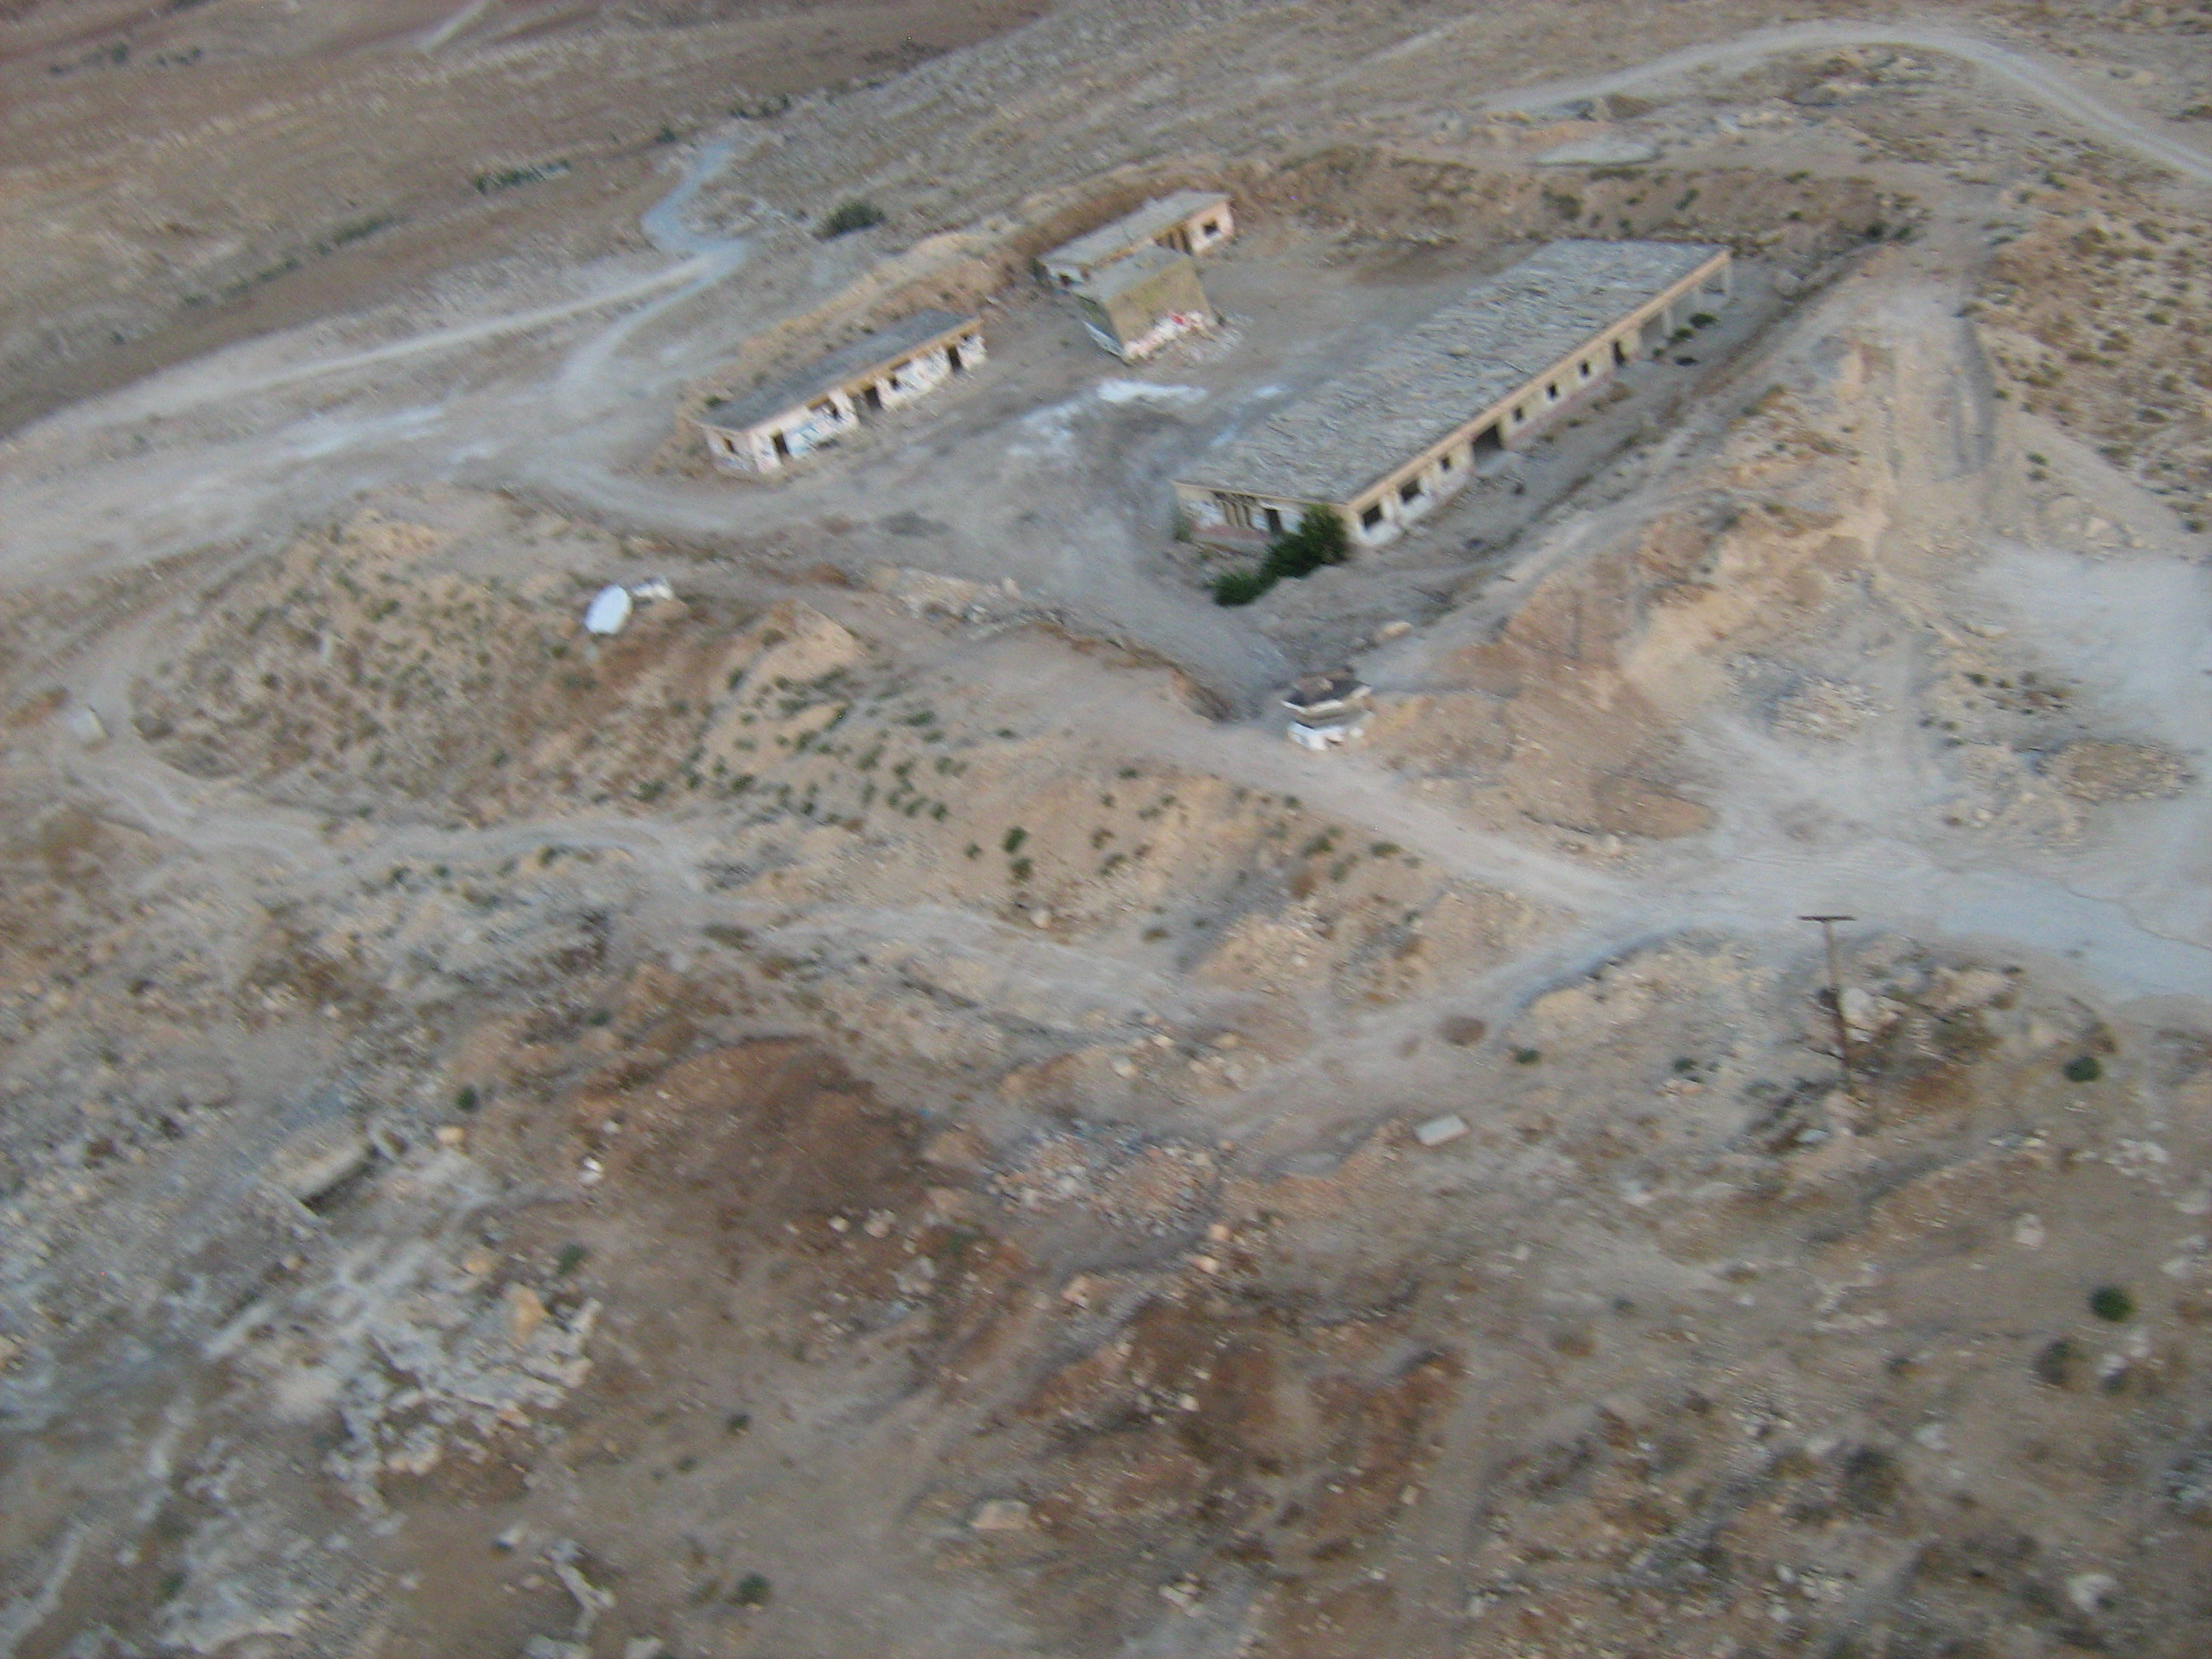
\includegraphics[width=0.45\textwidth]{images/maron-spy-satellite.jpg}
		\caption{Maron jokingly referred to this experiment in \ac{KAP} as the `first Palestinian spy satellite'. \cite{maron2008former}}
	\end{flushright}
\end{wrapfigure}

Of particular interest is Eric Wolf's thesis on the use of \ac{BAP} for `necrogeography', or the mapping of cemeteries, where he examined the accuracy and precision of various approaches to orthorectification.\footnote{See Section \ref{subsubsec:knitter} and Section \ref{subsec:precision}} as well as in comparison to high resolution GPS points. Wolf has been generous in contributing advice and even equipment to the Grassroots Mapping project. Also of note are Mikel Maron's attempts to use kites to produce maps in Palestine \cite{maron2008former} with \ac{KAP} techniques. However, few of these prior works have addressed the challenges in facilitation the adoption of such tools by non-technical participants, or in their potential to provide high quality map data to those without literacy in GIS technologies.  

The techniques I have refined in my own work have built upon these precedents, further simplified the assembly of a working kit, and attempted to devise methodologies for effective teaching of the techniques. In addition I have worked with others to push the limits of balloon and kite mapping in terms of altitude, resolution, speed of capture, and ease of image processing and map publication. These improvements will be discussed in the following chapter.

\chapter{The Grassroots Mapping tool chain}
\label{chap:toolchain}

\section{Balloon and Kite Aerial Mapping}

\begin{wrapfigure}{r}{0.5\textwidth}
	\begin{flushright}
		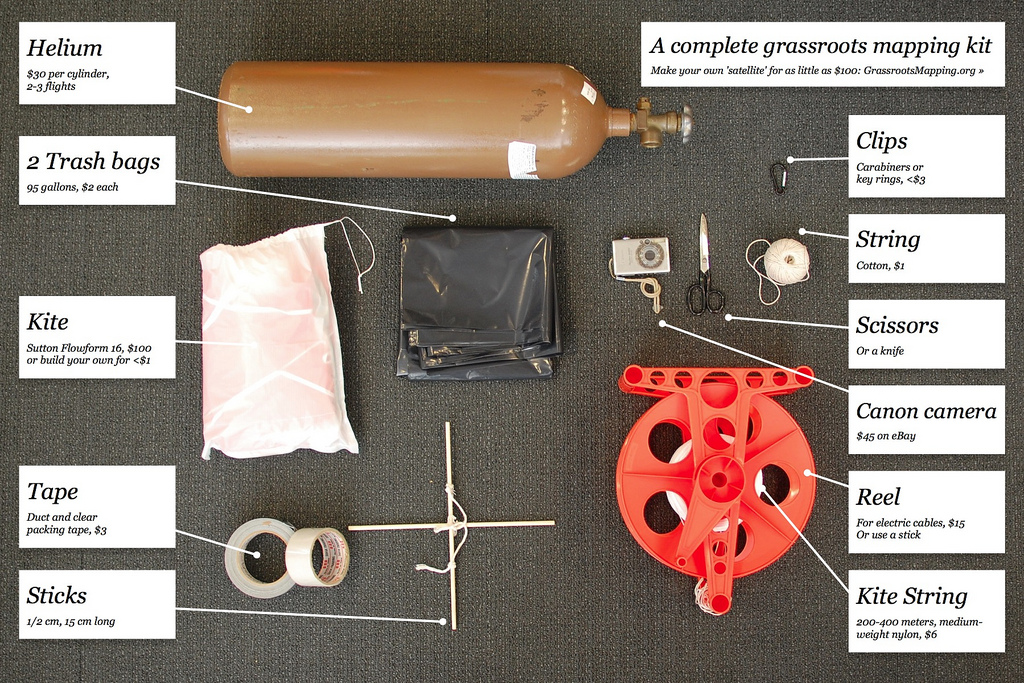
\includegraphics[width=0.45\textwidth]{images/100-dollar-satellite-poster.jpg}
	\end{flushright}
\end{wrapfigure}

As discussed in Section \ref{sec:aeriallowcost}, prior works in kite and balloon mapping make it redundant to discuss the advantages of such techniques beyond to say that they are easier and less expensive than aircraft or satellite-based imagery sources. However, the particulars of the equipment design developed for use in Grassroots Mapping projects emphasized yet lower cost, ease of use, and ease of reproduction than many existing designs, and a discussion of these decisions and the resulting designs is relevant. 

\begin{table}[tp] 
\caption{Comparison of balloon and kite mapping techniques. Despite the challenges and higher costs of balloon mapping, typical extents of a balloon map are far greater due to the higher altitude of flight, and due to a balloon's tendency to fly vertically in low winds, it is much easier to image the correct area. In the largest Grassroots Mapping project in the Gulf of Mexico, more than 60\% of maps to datewere made with balloons, and kite flights have typically had a much lower success rate.}

\label{aggiungi}\centering %
\rowcolors{1}{tableShade}{white}
\renewcommand{\arraystretch}{1.4}
\begin{tabularx}{\textwidth}{>{\bfseries}rYY}
\toprule\hiderowcolors
Type&Kite&Balloon\\\otoprule\showrowcolors
Altitude&300m&1400m\\
Extent&several hundred meters&\textgreater1km is common\\
Control&hard to target imagery - difficult in winds \textless45kph or \textless10kph&very fine control on windless days - difficult in winds \textgreater10kph\\
Payload&\textless2 kg&\textless300g\\
Time constraints&best winds in early afternoon&lowest winds at dawn\\
Portability&foil kites pack down to 1 liter size&helium tank and fragility of balloon limit portability, access\\
Tether angle&poor, camera altitude as low as 1/5 of tether length&in windless conditions, flies vertically; very sensitive to wind\\
Durability&excellent, no consumables&very poor; balloons pop regularly\\
Cost per flight&none&\$15-35 per flight dependent on helium costs\\
Initial total cost of kit&\$60-400 depending on kite and tether material&\$100-500 depending on choice of balloon and tether material\\\bottomrule
\end{tabularx}
\end{table}

Due to the distinct compromises of each technique, I recommend that those attempting to capture aerial imagery equip themselves for both scenarios. Luckily, the techniques share much of the same equipment, and it is possible in many places in the world to assemble a basic but complete kit for under \$150. I have done so in surprisingly unlikely locales, such as the West Bank in Palestine, Lima, Peru, and Kutaisi, Georgia. 

\subsection{Balloon mapping}

Helium is a limited and non-renewable resource, and obtaining it in the quantities necessary for aerial photography can prove challenging in the more remote parts of the world. 250 cubic foot tanks are most common, but are too heavy to carry without a wheeled dolly, and do not easily fit into cars or buses. They are also excessive, providing enough helium for between six and ten flights with a typical payload. If available, 80 or 120 cubic foot tanks are preferable, typically available in the United States for approximately \$45 and \$60, respectively. Those constructed from aluminum are especially convenient, being far lighter and easier to transport. Costs vary, depending on the distance from major helium sources such as the United States and Russia, but I have found large, 250 cubic foot tanks available for rental at approximately \$250 each in Bethlehem, in the West Bank, and for approximately \$300 in Lima, Peru, both at party stores. Gas supply vendors may offer somewhat lower prices, but sometimes require a permanent customer account, and can be reluctant to rent to non-industrial customers. 

\begin{wrapfigure}{r}{0.5\textwidth}
	\begin{flushright}
		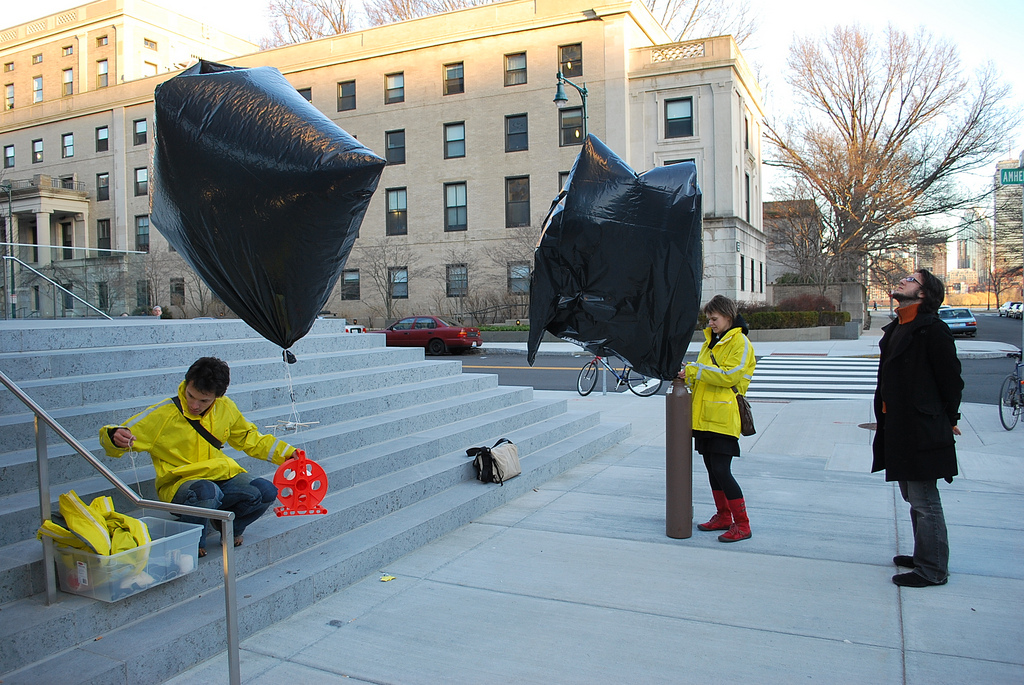
\includegraphics[width=0.45\textwidth]{images/trash-bag-ballooning.jpg}
		\caption{Testing trash bag balloons with the Department of Play working group on the MIT campus in Cambridge, Massachusetts.}
	\end{flushright}
\end{wrapfigure}

To further reduce costs, it is possible to use large high density polyethelene trash bags, of the kind typical worldwide. Two extra-large ninety-nine gallon bags suffice to lift a small camera and string to thousands of feet. Bags may be sealed shut with tape and filled without modification, or cut open and reassembled into tetrahedral shapes to minimize the surface area to volume ratio, providing greater lift. In addition, trash bags may be left inflated for several days without stretching or damaging the plastic, unlike latex balloons. However, helium leaks slowly through the plastic, and even relatively thick 2.7 mil plastic bags will lose most of their lifting power after a day or two. Trash bags are available for less than a dollar anywhere in the world, as is the clear plastic packing tape which may be used to seal them closed.  

\begin{table}[tp] 
\begin{threeparttable}[b]
\caption{Comparison of balloon type options}
\centering %
\rowcolors{1}{tableShade}{white}
\renewcommand{\arraystretch}{1.4}
\begin{tabularx}{\textwidth}{>{\bfseries}WYYY}
\toprule\hiderowcolors
Type&Cost&Typical \# of uses&Permeability\\\otoprule\showrowcolors
5-foot polyurethane advertising balloon\tnote{1}&\$US 140&hundreds?&Deflates 1-3\% per day\\
8-foot\tnote{2} latex weather balloon&\$US 25&up to 10 if careful&remains inflated for several hours; this weakens the balloon\\
Trash bags&~\$US 2&2-3&1-2 days if thicker (3 mil) plastic is used\\\bottomrule 
\end{tabularx}
\begin{tablenotes}
\item [1] Available from Southern Balloon Works, \url{southernballoonworks.com}
\item [2] `8-foot' denotes burst diameter, actual filled diameter during use is approximately 4 feet
\end{tablenotes}
\end{threeparttable}
\end{table}

\subsection{Kite mapping}

\begin{wrapfigure}{r}{0.5\textwidth}
	\begin{flushright}
		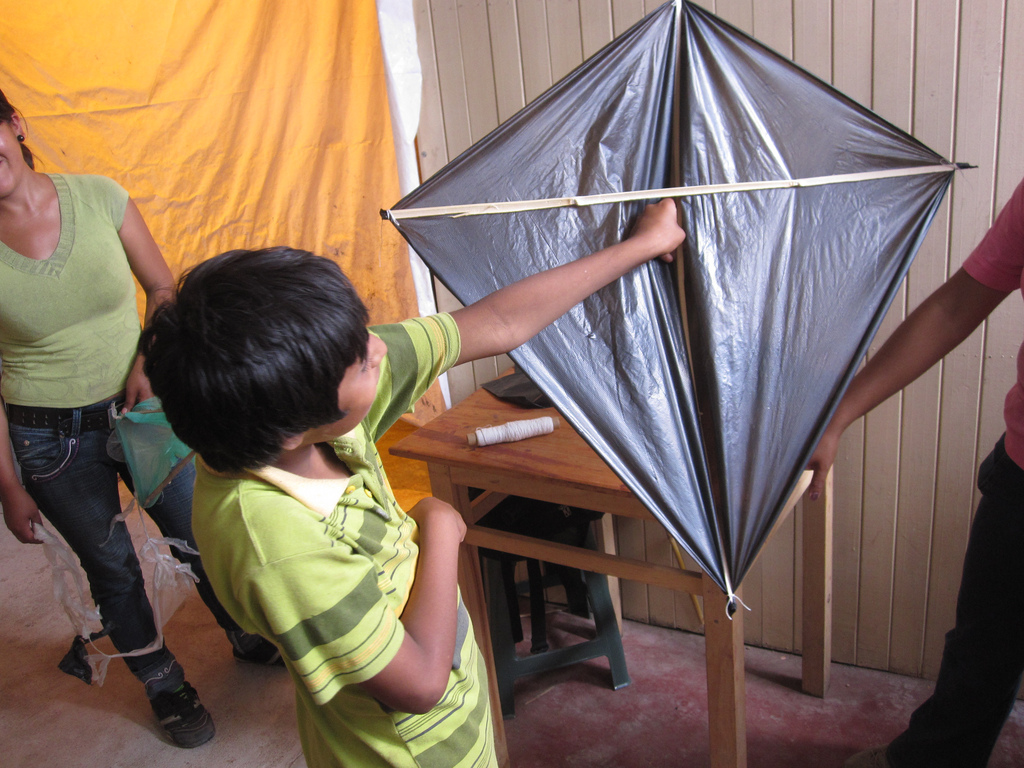
\includegraphics[width=0.45\textwidth]{images/kite-cesar.jpg}
	\end{flushright}
\end{wrapfigure}

Kites present an opportunity to loft cameras at near-zero cost --- materials for making kites can be found for less than a dollar, or recycled from waste. However kites can be particularly challenging to fly stably and difficult wind conditions often make for a frustrating and exhausting day of attempted map-making. With this in mind, I have looked to the experience of \ac{KAP} enthusiasts in choosing a respected standard in highly portable, reliable, and flexible flight: the Sutton Flowform. This `sled kite' has no rigid spars and even its 16 square foot model can be packed down to fit in a small sack. Flowforms can be flown at a wide range of wind speeds and the Flowform 16 can lift tens of kilograms in ideal conditions. However, its ~\$100 cost makes it somewhat beyond the means of many map makers. Therefore, whenever possible I have encouraged my collaborators to apply local traditional kite designs, often with great success. In Lima, Peru and Ramallah, Palestine, local designs were cheap and effective, the only issue being that they had to be scaled up to a size which could lift the approximately 300 gram payload. Kite building makes for an engaging and fun activity while reyling on local means of production for an aerial platform. 

\subsection{Camera and intervalometer}

Throughout the design of the Grassroots Mapping Kit I have emphasized low cost, therefore, taking a note from the page of low-cost aerial photographers like Oliver Yeh of \href{http://1337arts.com}{1337arts.com}, I recommend an inexpensive `point and shoot' camera, ideally of Canon's A or SD lines (the SD series is sold under the brand IXUS in Europe). While these tend to be in the 7-12 megapixel range, they are typically only 200-300 grams and are durable and compact. Such cameras can be found second-hand on \href{http://ebay.com}{eBay.com} for as low as \$US 50. Despite resolution, lens choice and stabilization advantages of more expensive models, consumer-grade compact cameras of this sort are widely available, and their image quality is sufficiently high that they make a good balance of weight, image quality, and cost --- the latter being of especially high importance since we have occasionally lost entire kits due to accidents such as improperly tied knots or sudden immersion in water. 

Canon consumer cameras also benefit from the active open-source hacking community's efforts to provide an alternative firmware with advanced features such as scripting. The \ac{CHDK}, which is stored on the camera's SD memory card, makes possible a script which I have adapted to trigger image capture every 5-10 seconds. The script, referred to as an intervalometer, is available for download at \url{http://wiki.grassrootsmapping.org/show/BalloonAerialPhotography}.  

\subsection{Enclosures and suspensions}
\label{subsec:cameraenclosures}

\begin{wrapfigure}{r}{0.4\textwidth}
	\label{fig:soda}
	\begin{flushright}
		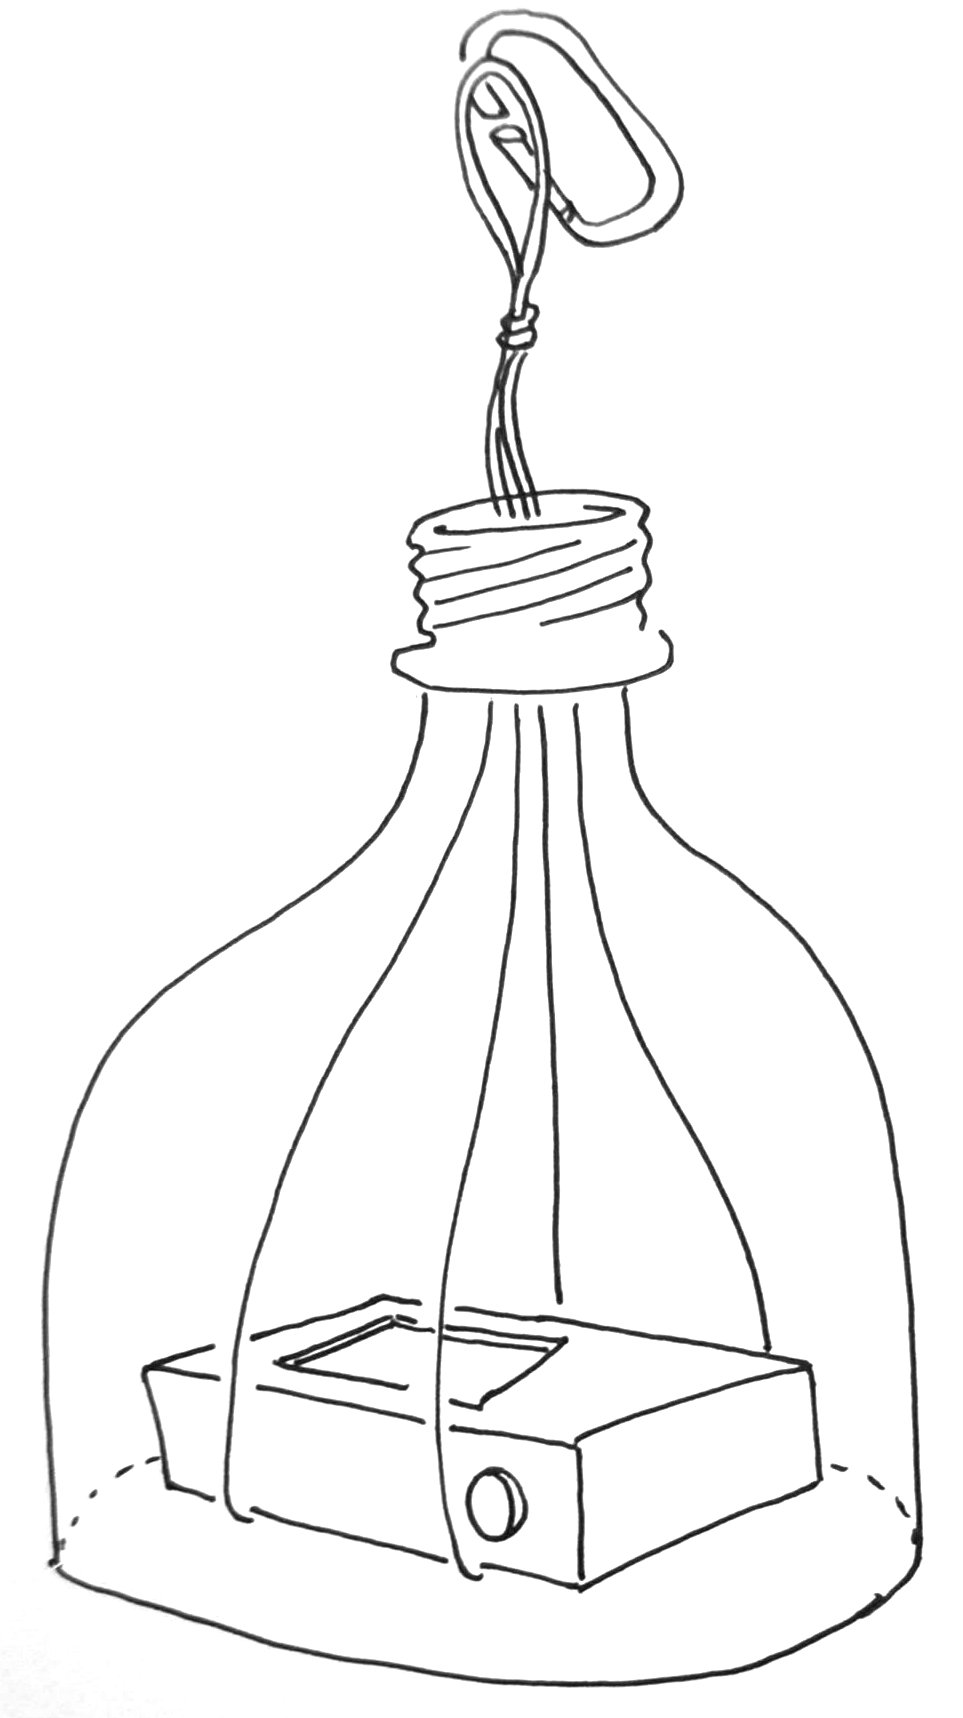
\includegraphics[width=0.35\textwidth]{images/soda-bottle-overview.jpg}
		\caption{The Soda Bottle Rig}
	\end{flushright}
\end{wrapfigure}

In order to attach the camera to the balloon or kite, \ac{KAP} enthusiasts typically make use of a `Picavet suspension', or arrangement of one continuous string on a series of rings or pulleys. This has the exceptional ability to keep the camera level and relatively stable even in turbulent conditions. However, experience in Peru\footnote{See Chapter \ref{chap:peru}} showed that constructing a working Picavet and maintaining it without tangles can be difficult for many, especially under adverse conditions such as long crowded bus rides, limited construction materials, and excited young participants. In the light of these challenges I have developed a more basic but still serviceable alternative called the `Soda Bottle Rig' which as an added feature protects the camera from light impacts. The basic design can be seen in Figure \ref{fig:soda}, and includes a pair of `wings' placed approximately 30 degrees apart, which serve to stabilize the enclosure against the wind, reducing radial blurring in the aerial images.

The soda bottle rig is convenient to carry, and makes immediate visual sense to observers, unlike the confusing array of crossed strings in the Picavet. The additional swaying of the Soda Bottle Rig in fact results in greater extent in the resulting maps, though resolution drops dramatically as photographs become more oblique. This does allow map-makers to decide whether to sacrifice consistent resolution in favor of a larger extent, however. In addition, while it works well for the typically horizontal tether of a kite, the Picavet suspension is rendered largely useless on a vertical tether, as the two mounting points are placed inline, one above the other. Still, experienced aerial photographers may achieve better results with the Picavet suspension in kite photography.  

\section{Reconceptualizing mapping interaction}

Once aerial imagery is captured, software must be used to distort or 'warp' the photos and combine them to fit a projection. This essentially maps every pixel of the source imagery to a position on the earth's surface, allowing for correlation to other maps and geodata sources. As no existing tool met all of the design requirements, such as cost, ease of use, low barrier to entry, and performance (see Section \ref{sec:existingtechniques}), I developed a unique tool and associated mapping framework with the goal of making DIY cartography simpler, cheaper, and more inclusive.

\subsection{Web-based orthorectification and warping}

In response to the collaborative design process and interviews conducted in Lima, Peru (Chapter \ref{chap:peru}), it was determined that the primary barrier to producing map imagery was the orthorectification process. While in Lima, participants made use of Adobe Photoshop CS3 as well as the Map Warper software discussed in Subsection \ref{subsec:mapwarper}. Attempts were made to instruct residents of the subject areas in the use of these tools. These techniques met with limited success due to factors such as availability of computers powerful enough to run Photoshop, latency in internet access, and most of all, the obscure interfaces which users were required to learn (see discussion in 9.1.9).  

Using Adobe Photoshop to manually disort and warp imagery over an imported base map was more direct and an easier process to explain, but the low availability of the software and the need for a powerful computer to perform large image transformations were additional challenges. The need for a lightweight, easy to use system became clear. The additional ability to run such a program in any standard web browser would put such tools within reach of anyone with access to an internet cafe.

\subsubsection{Cartagen Knitter}
\label{subsubsec:knitter}

The Cartagen Knitter software, developed in the months following the Lima, Peru mapping project, makes this possible. Using the Cartagen Framework along with an HTML 5 distortion technique prototyped by Steven Wittens of acko.net \cite{wittens2008projective}, I created an interface for users to upload images as overlays on an existing base map (typically OpenStreetMap vector data) and to manually distort an image by dragging the corners with the cursor. Tools for rotating, scaling, and adjusting the transparency of images were created, and the tool was tested and refined in a variety of workshops and mapping projects over several months. 

Cartagen Knitter makes several unique choices about how users rectify imagery. The first is that it emphasises orthorectification of individual images against a base map, rather than initial stitching of images into a larger composite image, then subsequent orthorectification and warping of that larger image. This decision was based on the relatively high computing resource requirements of manipulating a single higher-resolution image, given Knitter's emphasis on low-resource usage. Additionally, Eric Wolf of the US Geological Survey has found experimentally that the composite, or mosaic, technique suffers from a loss of accuracy: 

\begin{quote}
"The process of creating a single mosaic from the images and then geo-referencing wholly to the USGS High Resolution Imagery resulted in a reduction in accuracy of nearly 100\% in both location and orientation"
\cite{wolf2006lowcost}
\end{quote}

The second design decision which may seem curious is the emphasis on a completely manual orthorectification interface: no automated interest point finding or matching is used, despite the availability of such software (i.e. Hugin, Photosynth, Vision Workbench, etc.). Even Map Warper automatically warps images using the \textbf{gdalwarp} utility, though it asks users to identify common Ground Control Points to determine how to perform the warping. In practice, however, the use of such automated techniques did not result in good mosaic images, nor was the process of stitching, warping, and orthorectifying easy to understand or troubleshoot for non-technical users. Hugin provides for rectilinear warping, which does not assume a fixed camera position, but in order to successfully apply this configuration is essentially a `hack' and existing documentation is either unclear or no longer correct. Additionally, desktop programs such as hugin or Photosynth may be difficult to install in an internet cafe, which users in Lima might find necessary.

Discussion of rubbersheeting. \cite{white1985piecewise}

\section{Cartagen: an alternative architecture for digital maps}

Beyond the ability to orthorectify imagery, Cartagen is a fully-fledged cartographic scripting environment and renderer. It can draw vector data onto a pixel grid at over 10 frames per second on most computers, and follows the conventions of an animation framework rather than the more static assumptions of the typical mapping system. As the user interacts with a Cartagen map, features are drawn continuously. This negates the need to cache or otherwise store raster representations of map data, and sidesteps many of the assumptions and limitations of the modern mapping technology stack. This is also what makes possible the rapid feedback loop of the Cartagen Knitter, as there is no `render' or `warp' step --- the effect of the user's orthorectification is visible in real time. 

This alternative `geostack' is one of the most unique aspects of the Grassroots Mapping tool chain. The abilities it affords make it suitable for deploying original data without placing a high demand on technical skills or resources. 

(concurrent client ability)

- DIYDrones thread: "3 days stitching and tweaking images" \url{http://diydrones.com/profiles/blog/show?id=705844:BlogPost:134855&page=1#comments}

\subsection{Cartagen dynamic rendering}

As discussed in Section \ref{sec:webmapping}, most digital maps today employ a server-side caching mechanism providing a tiled image collection. The tiles are assembled seamlessly in the user's browser, and zooming is accomplished by maintaining multiple tilesets --- one for each zoom level. The resulting system scales predictably, as tiles do not vary dramatically in file size, and can be served using Apache or even stored locally. While this works well for a single dataset such as terrain contours, it commits the map to a single representation. Multiple tile sets can be stacked, and polygons can be overlaid, but most importantly, the user cannot edit the tiles or manipulate the data they contain. Compressing data into tiles strips them of their metadata and authorship information in favor of scalability and consistency. For companies such as Google or Yahoo, this represents a form of control over the map data; instead of distributing the source data, their use of tiles protects their intellectual property from re-use or adaptation. 

Diagram of Cartagen vs. Existing geostack

I designed Cartagen to sidestep many of these requirements, and to allow users to participate fully in the authoring of maps. Using new techniques made possible by widespread browser support for HTML5 and specifically the Canvas element, Cartagen can create maps which are not pre-rendered, but generated on-the-fly. This frees the map from a single projection or representation, and enables a more dynamic, interactive, and narrative cartographic style. Discrete vector data (made up of points, lines, and areas) can be downloaded in JSON format just once, and displayed at any scale and in any style. Recent increases in JavaScript execution speed [JavaScript speed stats] make possible relatively high framerates (~15fps on a typical machine), obviate the need for browser plugins like Flash or Java, and make dynamic HTML5 mapping accessible even on mobile devices such as on the iPhone, Android, and Windows Mobile platforms. As an added advantage, Cartagen performs much of the work of map display locally, reducing dependence on high-latency internet connectivity. It also allows users to easily download data and view or edit it offline. These features make it particularly appropriate for use in developing countries or in crisis situations. 

(usage restrictions in Google Maps and similar services)

\begin{wrapfigure}{r}{0.5\textwidth}
	\begin{flushright}
		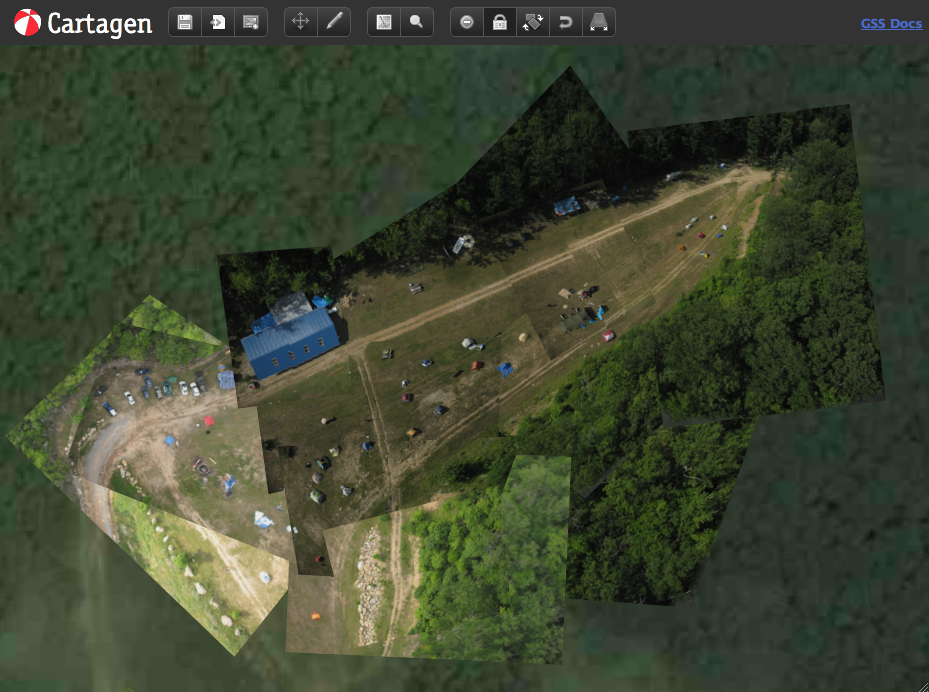
\includegraphics[width=0.45\textwidth]{images/knitter-wileys.png}
		\caption{A map of Wiley's Last Resort in Kentucky, produced in Cartagen Knitter with imagery captured from a remote controlled aircraft by Stewart Long.}
	\end{flushright}
\end{wrapfigure}

\section{Unique abilities}

Though other mapping frameworks such as OpenLayers have made use of the canvas element as well as other alternatives such as \ac{SVG}, Cartagen was among the first to appropriate the `content vs. display' paradigm of HTML/CSS, in order to allow users to style maps using a simple CSS-like syntax, known as \ac{GSS}. This took advantage of Cartagen's live-rendering ability to render features in response to simply defined, tag-based style definitions. Cartagen is one of the most easily customizable map rendering frameworks, and is specifically designed to leverage literacy in HTML/CSS, thereby lowering barriers for those interested in using geospatial design tools. 

(GSS illustrations)

As a fully scriptable cartographic environment, Cartagen was also uniquely suited for building an image orthorectification tool. The Canvas element is essentially a pixel raster, but because Cartagen's primitives are vector objects stored as points and polygons, it there is no need to store resampled source imagery while performing distortions or transforms. While in Photoshop, a powerful computer is required to store, manipulate, and export a map of any considerable size (maps made for the BP oil spill project were over 50,000 px in each dimension), Cartagen can be used to orthorectify using a laptop or even a low-power netbook. Users in effect see a lower-resolution preview rendered only at the size of their browser window, and a final, high-resolution composite image is created using ImageMagick on the server side. This lowers the cost of the equipment to process and orthorectify aerial imagery by thousands of dollars. 

Cartagen makes use of open standards such as JSON, OSM-XML, and GeoJSON, and can be used to generate \ac{GeoTIFF}s or even a \ac{TMS} tile service. In addition, because it can store and display both raster and vector data, once images are rectified, the pen tool can be used to trace streets, buildings, and borders. However, for those interested in using Cartagen Knitter to produce data for OpenStreetMap, the non-standard TMS required for map editors such as JOSM is also available.

\begin{wrapfigure}{r}{0.5\textwidth}
	\begin{flushright}
		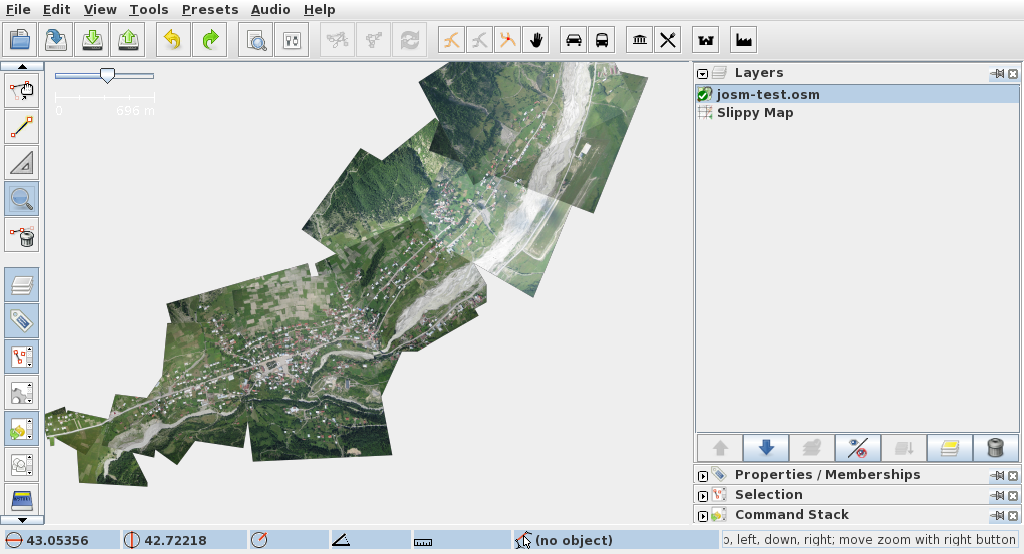
\includegraphics[width=0.45\textwidth]{images/knitter-josm.png}
		\caption{Viewing output from the Cartagen Knitter in \ac{JOSM} for contribution to the OpenMapCaucasus project in Georgia. Read more in Section \ref{subsec:georgia}}
	\end{flushright}
\end{wrapfigure}

\subsection{Why an entirely new mapping system?}

In a sense, rendering is at the heart of the argument for critical cartography. If mapping is to be a means to advance an agenda, or develop a narrative, or create a communal self-image, it must allow for diverse forms of representation. We have the divergent data and the means to collect, collate, and publish it – what we lack is a way to represent it in layered, interactive, and radically unique ways. 

Cartagen's unique architecture allows it to describe a constantly changing data set, an ability which is both technologically advantageous and epistemologically transformative. Once maps are rendered in the browser window instead of by Google or Yahoo, users are empowered to design, interpret, manipulate, and publish that data in new and compelling ways. 

\section{An iterative toolchain development process}

In order to develop tools which respond well to user needs, I followed a collaborative process, testing various tools in a variety of contexts. Various combinations of tools were tested with participants from Lima, Peru, New Orleans, and Rock Creek, West Virginia. Interviews and notes were used to develop new tools which built on the strengths of existing and off-the-shelf systems such as Photoshop, Hugin, and Map Warper. The same is true for the physical tools such as the balloon and kite kits, including the camera housing, reel construction, and auto-triggering setup. 

\begin{wrapfigure}{r}{0.5\textwidth}
	\begin{flushright}
		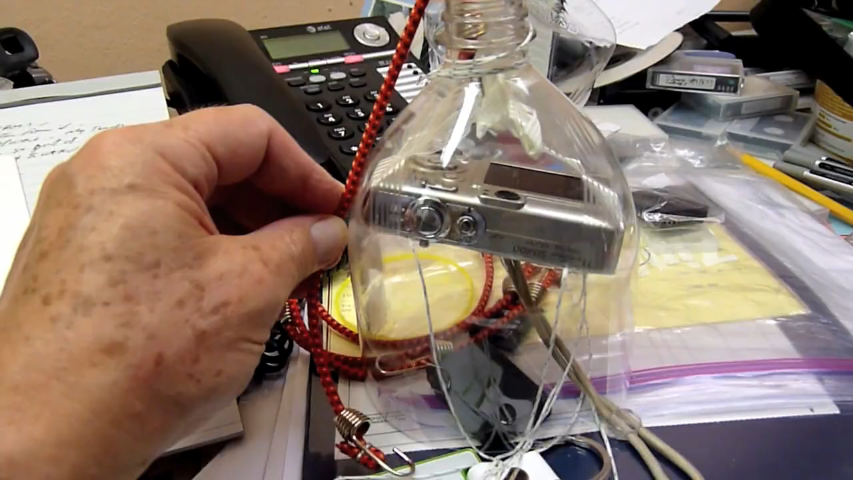
\includegraphics[width=0.45\textwidth]{images/pat-coyle-video.png}
		\caption{Still frame from Pat Coyle's demonstration on YouTube \cite{coyle2010sodabottle}}
	\end{flushright}
\end{wrapfigure}

In the case of the camera housing, Grassroots Mapping community members have iterated and improved upon the soda bottle enclosure, discussing and testing alternatives on the mailing list, and even posting videos of tests. Pat Coyle, a mailing list member, published a narrated demonstration of a soda bottle enclosure with improvements such as a window to access the camera controls and a small bungee cable to stabilize the camera against the inside of the bottle. In another example, Mathew Lippincott prototyped solar-powered hot air balloons constructed from painter's plastic sheeting, conducted pigmentation and lift tests to determine suitability for carrying cameras. The tests and builds were held at a public event in Portland, Oregon, and videos and instructions were posted online.

\begin{wrapfigure}{r}{0.5\textwidth}
	\begin{flushright}
		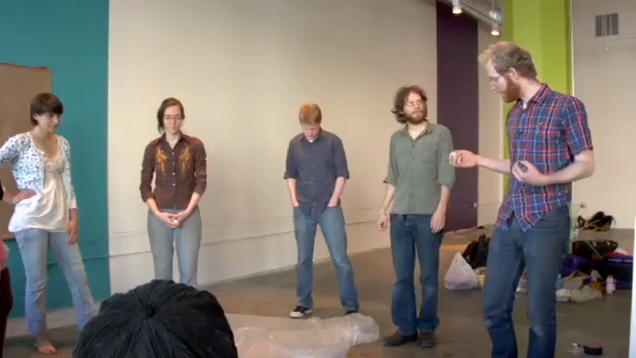
\includegraphics[width=0.45\textwidth]{images/lippincott-workshop.png}
		\caption{Mathew Lippincott leads a workshop entitled `Grassroots Mapping PDX' where participants constructed and tested solar and helium balloons made of plastic sheeting, for use in the Gulf of Mexico.}
	\end{flushright}
\end{wrapfigure}

Regular testing of new tools at the MIT campus, as well as repeated attempts to orthorectify the resulting imagery, grounded the software development in concrete usage and experience, and a workshop at the Google campus in Mountain View in April 2010 included a collaborative hacking session aimed at identifying and resolving bugs and adding new features in direct response to the day's mapping efforts. 

\begin{wrapfigure}{r}{0.5\textwidth}
	\begin{flushright}
		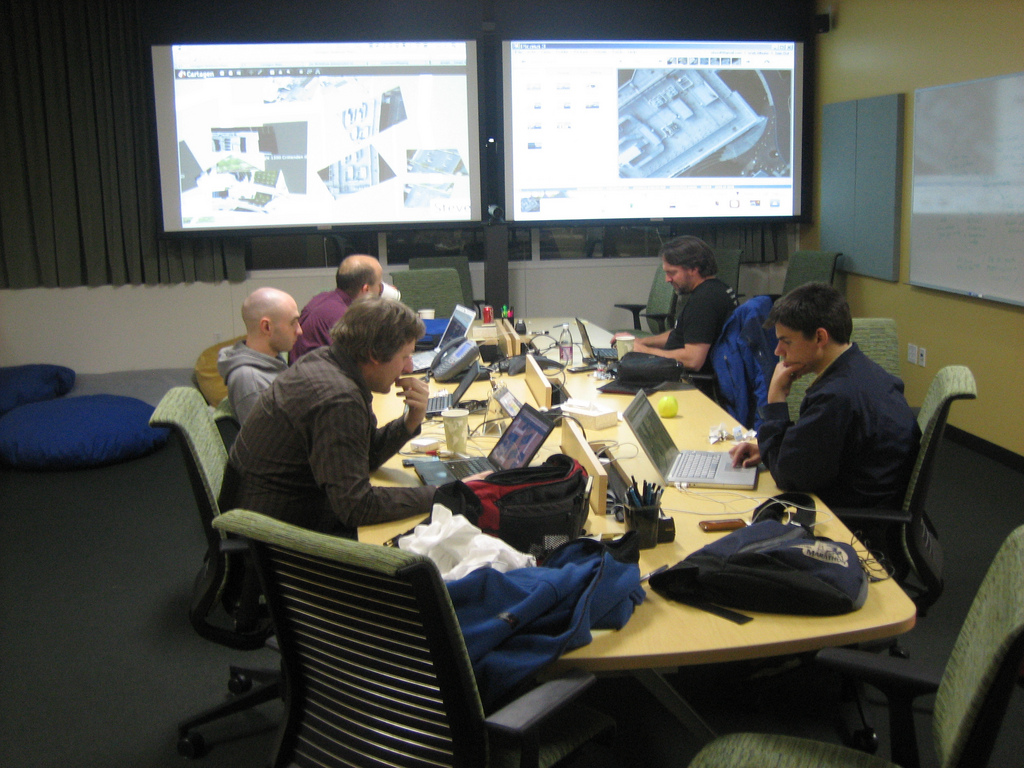
\includegraphics[width=0.45\textwidth]{images/asynchronous-editing.jpg}
		\caption{Collaborative editing of a map of the Google campus using Cartagen Knitter at the WhereCamp 2010 unconference. User feedback was incorporated into the tool and re-deployed in real time.}
	\end{flushright}
\end{wrapfigure}

As development of the Cartagen Knitter software progressed, mailing list members with a variety of needs chipped in with suggestions, bug reports, and feature requests, including the ability to lock images when finished warping, revert to original image proportions, and use keyboard shortcuts for common commands. Combined with test flights and experimentation by active community members such as Pat Coyle and Mathew Lippincott, the tools have progressed from partially functioning prototypes to relatively mature technologies with known limitations and parameters. It was the multiple deployments of the tools in the Lima, Peru and BP oil spill case studies, however, which put them to the test in real-world applications, and forced us to push the tools' abilities to their limits. 

\chapter{Case Study: Grassroots Mapping in Lima, Peru}
\label{chap:peru}

\section{Introduction}

In the interest of basing tool development and design on real-world applications, and due to an ongoing conversation with Carla del Carpio of Lima-based Manzanita "A", I travelled to Lima, Peru in January 2010 to work with several informal settlements and a number of NGOs on Grassroots Mapping projects. From the start, this was considered an experimental program, where Peruvian collaborators would help to better define needs and to iterate and improve upon the balloon and kite imaging techniques.

\begin{wrapfigure}{r}{0.5\textwidth}
	\begin{flushright}
		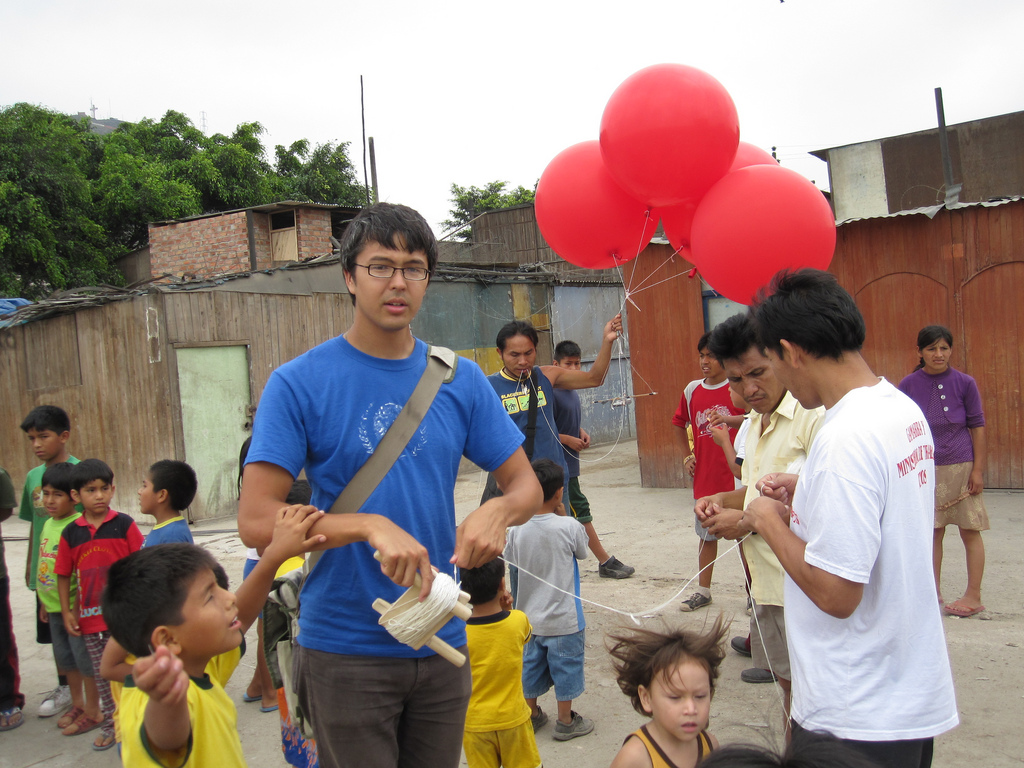
\includegraphics[width=0.45\textwidth]{images/kids-canta-gallo.jpg}
		\caption{Children capturing aerial imagery in Canta Gallo, Lima, Peru.}
	\end{flushright}
\end{wrapfigure}

The program was also explicitly educational in its goals, and with educators from Lima-based Centro de Información y Educación para la Prevención del Abuso de Drogas (CEDRO) and Manzanita "A", a curriculum was developed to involve local youth in the mapmaking process. We placed emphasis on examining the cartographic process with students not only in the sense of recording the present layout of students' communities, but with the intent to depict and discuss geography in the context of the history and future of the communities. A series of exercises were devised to situate mapping as a way to examine and reflect upon rapid urban growth and participatory urban planning such as occurs in the partner communities.

This alignment of map-making with education and youth empowerment was not new, but for the first time it was one of the primary goals of the project. Mappers often ask me why I work with kids; educators, on the other hand, rarely ask why I focus on mapping. To answer the former, there are a variety of reasons, but one of the main reasons is that kids are good mappers. They represent a wealth of knowledge about the very details of a community which adults are likely to gloss over. They have the attention span, the patience, and the enthusiasm, and are often more open-minded and creative than their adult cartographic colleagues. They bring a unique point of view to map-making, taking less for granted about their geography, and stand to learn a great deal from such a combination of the physics of flight, the mathematics of cartography, the history of urban development, and the political implications of their physical world. Making maps of such quality and utility with school children highlights the ease with which such maps can be made to skeptical adults. Finally, pragmatically, it can be hard to use balloons and kites in any populated area \textbf{without} including kids, as they usually come out of the woodwork, eager to participate. There is a sense as well that everyone becomes a child when flying balloons and kites, and certainly the presence of a large group of eager kids tends to ease the inhibitions of curious adults, encouraging them to loosen up and take part in the fun. 

`learn to see themselves as competent and confident members of their community. Children and adolescents appreciate the opportunity to feel that they can play a useful role in community or environmental improvement.'

\href{http://www.unicef.org/teachers/researchers/intro.htm}{Curriculum on ``{}Children as Community Researchers''{}} - UNICEF, authored by \href{http://web.gc.cuny.edu/che/cerg/about_cerg/environmental_learning_index.htm}{Children'{}s Environment Research Group}

\href{http://training.esri.com/campus/library/bibliography/RecordDetail.cfm?ID=95545&browseonly=0}{Mapping in a Shoebox} - A Grassroots Approach for Developing the Geospatial Literacy of Elementary Children - 24th International Cartographic Conference - Jaqueline M. Anderson, Sally Hermansen, Lorraine Innes, 2009

The selection of Lima as a site for prototyping and collaboration was also due to the favorable bureaucratic climate. Because of the land-ownership situation discussed in Section \ref{sec:twoworlds}, the Lima project was also intended to provide easy and inexpensive alternative means for communities to produce maps specifically for tenure claims. It was believed by myself and the other project planners that it would be possible for partner communities to submit such maps to the relevant authorities\footnote{An organization known as \ac{COFOPRI}, whose mission is to `Execute the actions of generating property rights ...' (`Ejecutar las acciones de generación de derechos de propiedad predial que otorguen seguridad jurídica permanente y que sean sostenibles en el tiempo.') Citation needed.} as part of the official tenure claims. However, we felt that this agenda should be secondary to the educational goals we established, and to emphasize the benefits of process over end product. Further discussion cemented our belief that as non-residents --- who would not be affected by the legal outcomes -- it was not our place to aggressively advocate such uses. 

\subsection{The Other Path: Lima's history of informal settlement}

Lima's unique history made it an especially suitable choice for participatory mapping on a cultural level. Lima has expanded over the last century to include a full third of the population of Peru, in what has become a process of continuous and transformative growth. The result is a city in which large tracts of land have been settled 'extralegally', a term borrowed from Hernando de Soto's exhaustive history of the city in `The Other Path'. These settlements are known locally as `invasions' due to their inhabitants' sense of having not only literally seized the land from private landowners or the government, but of having unilaterally constructed a working alternative to the official municipal government, including public works, tax collection, and education. These communities, typically made up of only a few hundred people each, are truly apart from the central government, and only through a years-long process are able to gain title to their land along with basic services such as plumbing and electricity.

De Soto paints a picture of a government entirely overwhelmed by the floods of immigrants from rural areas, and entirely unable to accommodate these newcomers in its infrastructural or bureaucratic capacity. `We appear to be witnessing', he writes, `the most important rebellion against the status quo ever waged in the history of independent Peru.' The numbers are stunning; even at the time of his writing in 1987, he describes in detail how `...through invasions or illegal aquisitions of land, neighborhoods sprang up which today account for 42.6 percent of all housing in Lima and are home to 47 percent of the city's population.' \cite{desoto1987sendero}

This situation, though not unique in the world, is especially appropriate as a place to attempt a mapping project which acts both outside of traditional cartographic means of production, and outside the conventional framework of GIS. In the months that followed the Lima project, I began to refer to the tools and techniques which were prototyped in Lima as a kind of `DIY satellite', and that seems fitting given that in the invasions of Lima, residents are accustomed to Doing Everything Yourself, from constructing roads to building and maintaining their own plumbing. In addition, any means to reduce the barriers to acquiring tenure is held in high value; de Soto's research shows that the market value of a plot of land increases ninefold when its owner receives official title. As in many urban slums worldwide, most residents do not have a bank account; their home represents their primary means of storing wealth. Land title becomes a form of valuation, and makes it possible to sell one's plot, or use it as collateral for a loan. More than anywhere else, cartography is inextricably connected to basic systems of value in the invasions, making them an exciting place to test a more participatory means of making maps. 

Additionally, we identified a number of more immediate applications for an up-to-date map. Both CEDRO and Manzanita `A' looked forward to using the map for research and planning purposes for their ongoing projects in the settlements. The maps could also be used to support decision making amongst community leaders, for public works projects, land use discussions, and even for promotional purposes. Simply providing another means for community members to gain access to a map would allow them to compare it to the `official' version, or to independently verify that the community was in fact built to their agreed plot divisions. Finally, the process of making the map would build literacy in cartography and give participants more say in how their community is represented to the outside world.  

\begin{wrapfigure}{r}{0.5\textwidth}
	\begin{flushright}
		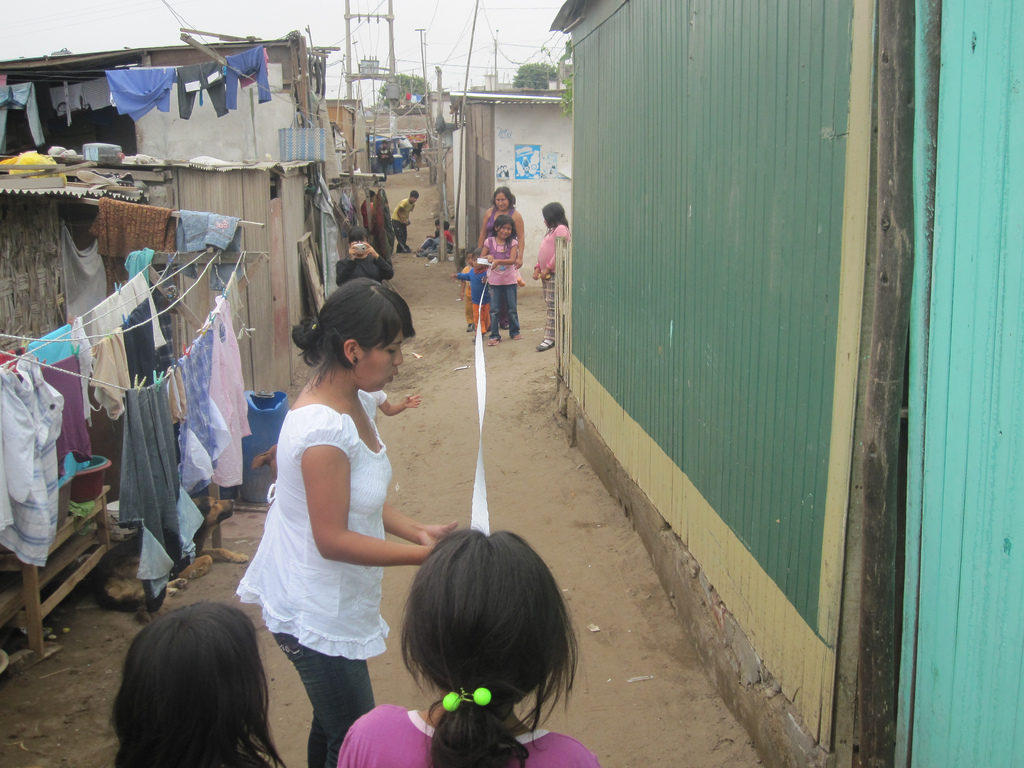
\includegraphics[width=0.45\textwidth]{images/juan-pablo-measuring.jpg}
		\caption{Measuring homes with a paper measuring tape in Juan Pablo II, Lima, Peru.}
	\end{flushright}
\end{wrapfigure}

\subsection{Mapping with Juan Pablo II}

Both Manzanita `A' and CEDRO were enthusiastic about the potential of a mapping project from the outset, and Carla del Carpio coordinated with CEDRO's Ernesto Fernandez to set up a 6-day program, or `Projecto Integral' with a group of approximately a dozen students in the Juan Pablo II settlement in Lima's Villa el Salvador district at the south end of the city. Each day of activities, held between January 12 through 28th, lasted from 11am until approximately 3pm. 4-6 CEDRO instructors and 2 from Manzanita `A' attended, and the twelve of so students ranged from 8 through 14 years old. The Juan Pablo II community consists of approximately 6 blocks of homes arranged in a loose grid, though this was not apparent from the Google Maps imagery, which we dated to approximately 2006, or 4 years earlier. The community was 5-6 years old, and many but not all of the students remembered when their families had first come to the site. 

We began the workshop with an introduction to map making, by asking students to work together to draw their community. This resulted in a variety of means of representation, though through prompting, they tended increasingly toward birds-eye view. Even then, some experienced difficulty with collaborating at a common scale, with some adjustments and redrawings occurring once each student's map intersected their neighbor's. Next, students enthusiastically constructed measuring tapes and we broke into groups to literally measure the homes. 

An attempt to show the existing Google Maps imagery and to ask students to identify their homes or even the entire community in a map were not successful; the maps did not seem relevant to participants, as most students seemed not to have a high degree of computer literacy or exposure to the internet. 

\subsubsection{First flights in Juan Pablo II}

Interested in quickly capturing aerial imagery and moving on to analysis, we begin flying balloons on the 14th of January. Four balloons, each of approximately 3 feet in diameter, were attached to a Picavet suspension (see Subsection \ref{subsec:cameraenclosures}) and launched on a 500 foot long tether of nylon kite string. Winds of over 10 mph prevented us from capturing many images from high altitude, and frustratingly, this continued to be the case for several subsequent sessions. 

\begin{wrapfigure}{r}{0.5\textwidth}
	\begin{flushright}
		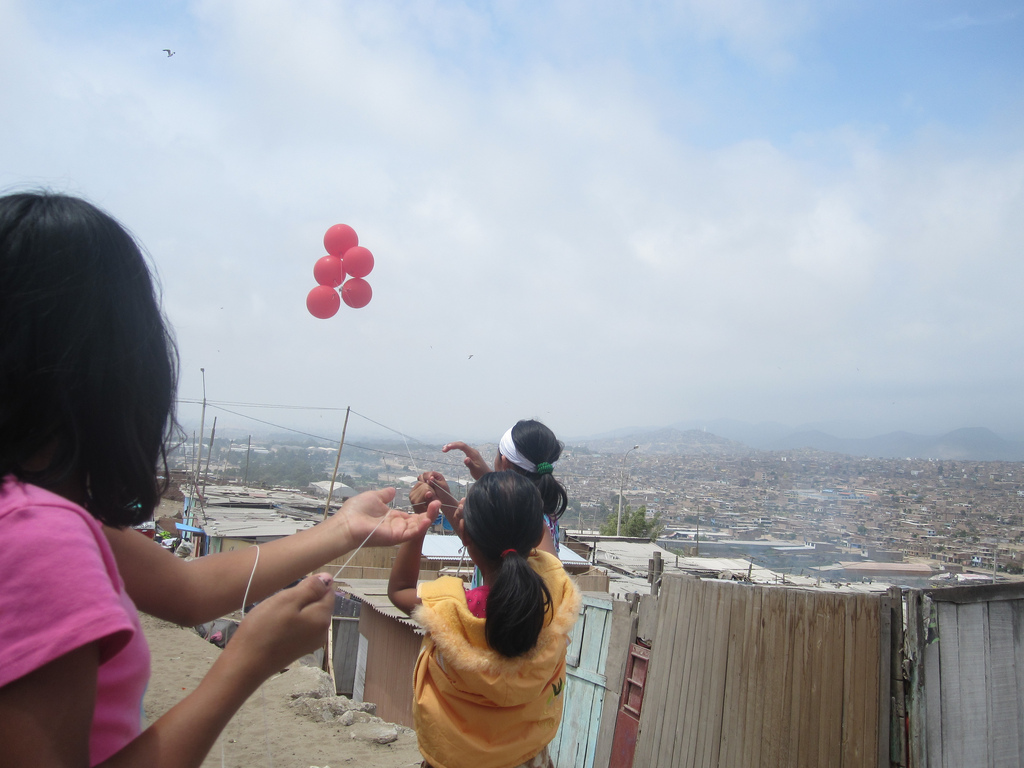
\includegraphics[width=0.45\textwidth]{images/juan-pablo-first-flight.jpg}
		\caption{Initial balloon flights in Juan Pablo II.}
	\end{flushright}
\end{wrapfigure}

Involving the students as full participants, or actors, in the process was also difficult, as only one or two people could hold the balloon at a time, and it required several minutes of experience before students were confident enough to reel the tether on their own. Juan Pablo II is positionen on a southward facing hillside, and the kites flew at a very shallow angle --- close to the ground -- as wind blew northward over the ridge. We attempted a variety of kites and launch locations. 

On the 26th, after several more attempts with both balloons and kites, we captured several uesable images of the community, and together with Carla del Carpio and Ysabel Luisa of Manzanita `A' I stitched together the images into the best and most up-to-date map yet of Juan Pablo II.  

\begin{figure}[h]
  \begin{center}
	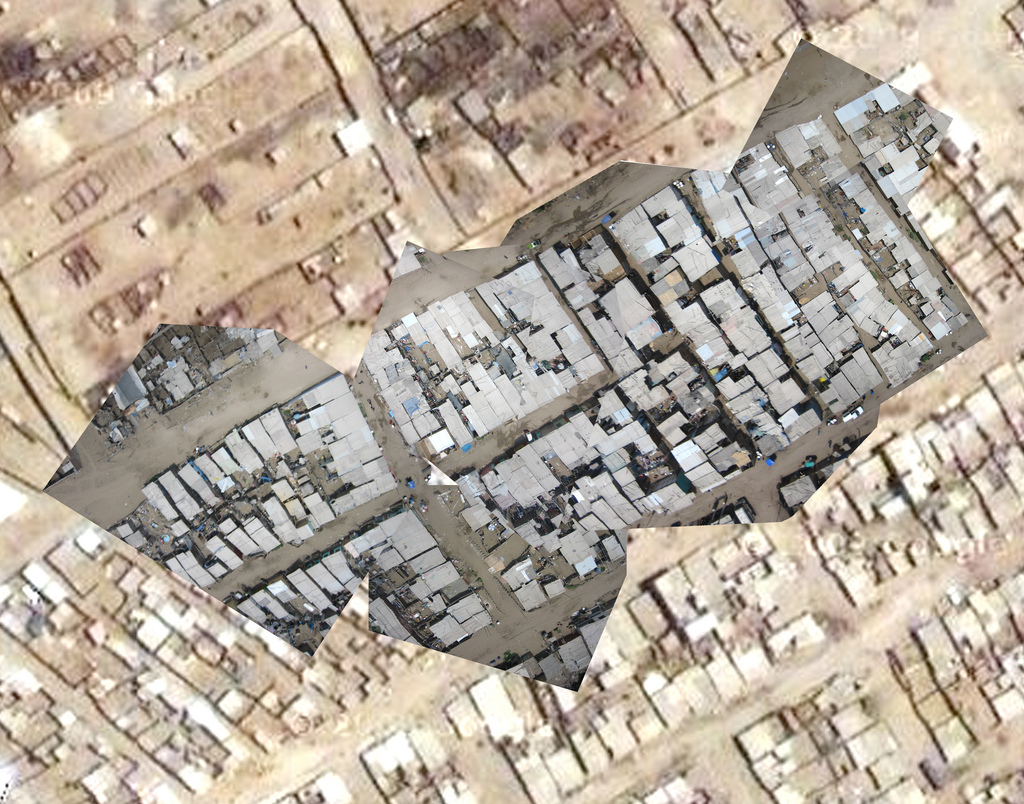
\includegraphics[width=1\textwidth]{images/juan-pablo-final.jpg}
	\caption{Completed balloon map of Juan Pablo II, produced with Adobe Photoshop CS4}
  \end{center}
\end{figure}

\subsubsection{Situating mapping practice}

Establishing a rapid feedback loop with participants is of paramount importance, especially when they are dependent on external aid for part of the map-making process. In Juan Pablo II, the line between `researcher', `cartographer', and `participant' was blurred, as all parties were learning to create maps in a novel process. Throughout the flights, we made regular prints of the aerial imagery we were able to take and shared these with the participating students. Many of the most popular were taken from only a few dozen feet high, but showed the students and their immediate environment from a new perspective. 

However, while we awaited a major success in capturing imagery (a success which took 14 days to achieve), the students were engaged in other projects. Beyond discussing and drawing maps of Juan Pablo II, students interviewed their parents and presented drawings and short reports on the history of the settlement. This resulted in some cases in very detailed accounts of how homes began as straw `caracoles' or tents, and progressed to wooden, metal, and even brick structures. One student named Frank recounted what year his family received electricity and when they began planting a garden. While these details may be exciting to hear from a historical, anthropological, or aid perspective (I had received specific requests from a cartographer from the World Bank for details on house construction), for myself and my fellow teachers, it served the more important role of contexualizing the current state of the settlement --- for the students -- in a years' long process of construction and reinvention. It also emphasized the time dimension of mapping, which is often neglected, but in areas of such rapid change, can render mapping efforts irrelevant within just a few years. Indeed, the maps we were beginning to produce from aerial imagery showed that those available on Google Maps were so old as to omit entire roads and buildings.

\begin{wrapfigure}{r}{0.5\textwidth}
	\begin{flushright}
		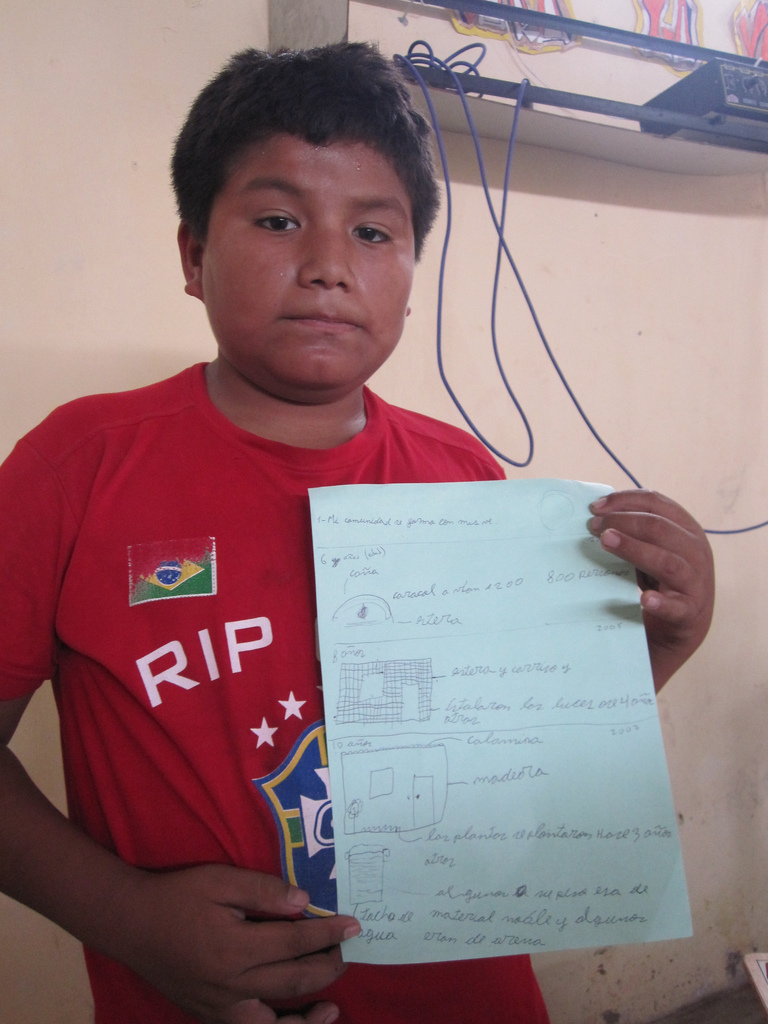
\includegraphics[width=0.45\textwidth]{images/juan-pablo-frank.jpg}
		\caption{Frank, a student from Juan Pablo II, presents a detailed history of infrastructural improvements to his home.}
	\end{flushright}
\end{wrapfigure}

We then asked students to produce similar work --- drawings and written reports -- on how they imagined the community might look in the future. We asked in this case for a depiction of the entire settlement, and were surprised when two students brought back a three dimensional model of Juan Pablo II, set seven years in the future. While the early aerial images and mapping exercises had prompted many students to depict their community in a bird's-eye view, this maquette revealed a wealth of detail related to wealth, quality of life, and an awareness of family needs. Unlike in present-day Juan Pablo II, the model depicted many two or three-story buildings -- signs of long-term tenure and financial stability, or even rental income. The buildings were largely depicted as brick, and many had stores, such as a hair salon or a flower shop. An especially interesting feature was a `Wa wa wasi', or day care center, which did not exist in present-day Juan Pablo II, but which allows two parents to work normal hours while their youngest children are cared for. Paved roads, plantings, and a soccer field completed this ambitious plan for the settlement.

\begin{figure}[h]
  \begin{center}
	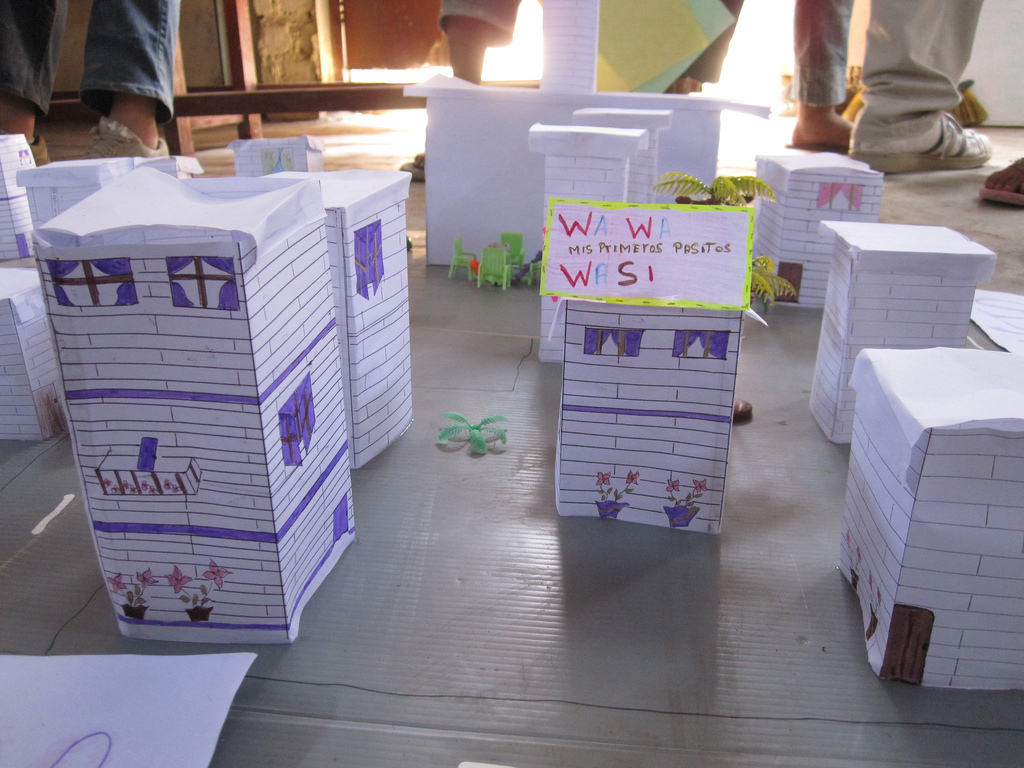
\includegraphics[width=1\textwidth]{images/juan-pablo-maqueta.jpg}
	\caption{3D paper model of the future of Juan Pablo II.}
  \end{center}
\end{figure}

This kind of map-making recalls the 3D Model Mappipng or Ground Mapping traditions of PGIS practice, with an emphasis on community assets and the explicit link between mapping and urban planning. The ability to view the model both from above as we were doing with balloons in the \textbf{real} Juan Pablo II, as well as from a first-person perspective by planting one's head amongst the buildings, bridged the gap between the abstracted god's-eye view and the situated personal view of the settlement. The model was extremely popular amongst not only the rest of the students and teachers, but amongst the parents and community leaders who attended our final presentation. 

\subsubsection{Stitching maps with Juan Pablo II}
\label{subsec:stitchingjp2}

Throughout the balloon and kite flights, we employed various techniques to process the aerial imagery into maps. Starting with the \begin{wrapfigure}{r}{0.5\textwidth}
	\begin{flushright}
		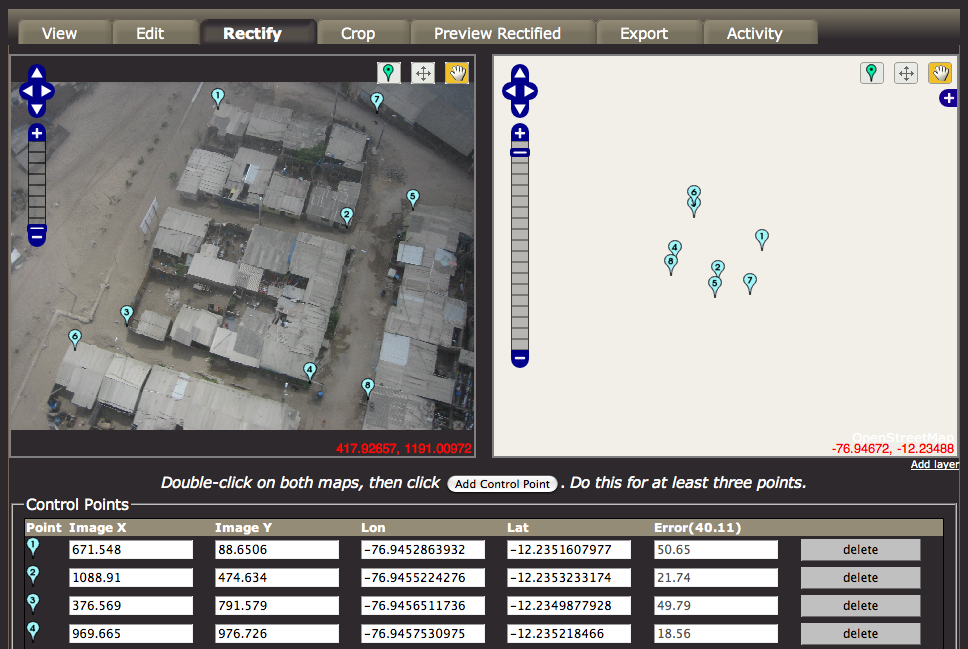
\includegraphics[width=0.45\textwidth]{images/map-warper.png}
		\caption{The Map Warper interface for identifying Ground Control Points. \cite{waters2009warper}}
	\end{flushright}
\end{wrapfigure} Map Warper software available at \url{http://warper.geothings.net}, teachers from Manzanita `A', we switched to Adobe Photoshop after a few attempts. Designed for printed maps, Warper experienced difficulty successfully warping some of the more oblique or distorted imagery, and in order to compensate, GCPs had to be placed deliberately incorrectly in a laborious trial-and-error process. (See Subsection \ref{subsec:cameraenclosures} for an overview of Map Warper). \begin{wrapfigure}{r}{0.5\textwidth}
	\begin{flushright}
		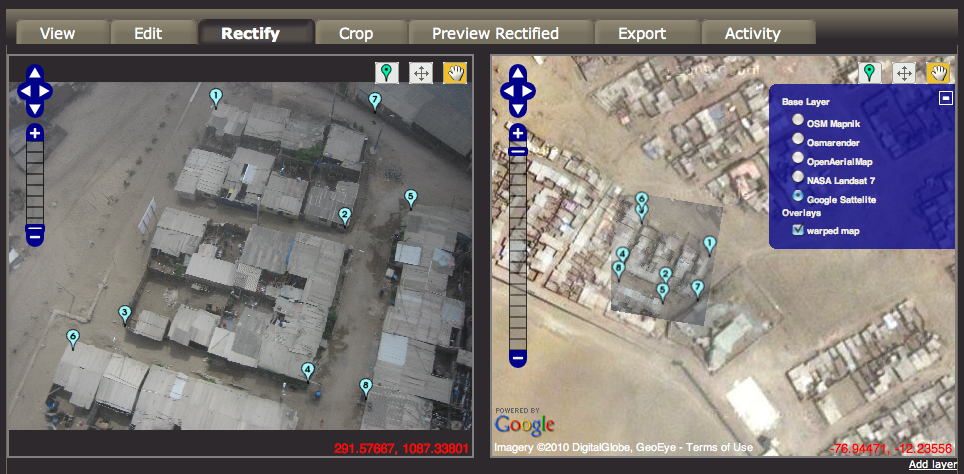
\includegraphics[width=0.45\textwidth]{images/map-warper-hack.png}
		\caption{Demonstration of JavaScript hack to insert Google satellite data for warping in areas with low feature density. \cite{waters2009warper}}
	\end{flushright}
\end{wrapfigure}Additionally, Warper uses OpenStreetMap tiles as a base layer, but in Juan Pablo II and other areas we worked in around Lima, there was no data available, and we were forced to use a JavaScript hack to insert Google satellite imagery or another viable source. Even then, it proved difficult to successfully stitch a map, as multiple steps separated an assignment of GCPs with the feedback that an image was successfully warped. This is not to say that Map Warper is not a valued tool for its intended use, and in fact Shekhar Krishnan more recently applied it successfully in digitizing paper maps of Mumbai. However it was not suitable for much of the aerial imagery we gathered, and proved difficult for those with limited computer fluency.

Our next tool was Adobe Photoshop CS4, which can yield impressive results for an experienced user (see GonzoEarth, Subsection \ref{subsec:gonzoearth}). This proved to be a workable alternative, where we used the Distort and Warp tools to align images in separate layers over a base image taken from Google Maps or another source. The total process for stitching 12-15 images took approximately 2-3 hours. Though not a GIS tool, Photoshop has the benefit of being fairly easy to find, though in fact none of the teachers I spoke with had a copy. Still, the use a generalized tool has the benefit of encouraging the learning of generalizable skills, and can result in a more inclusive process. PGIS researcher Peter Poole notes that in order to build a map-making capacity in areas of low computer literacy, `tracing was chosen over digitisation, and simple graphics software over geographic information systems (GIS).' \cite{poole2006there}

\begin{wrapfigure}{r}{0.5\textwidth}
	\begin{flushright}
		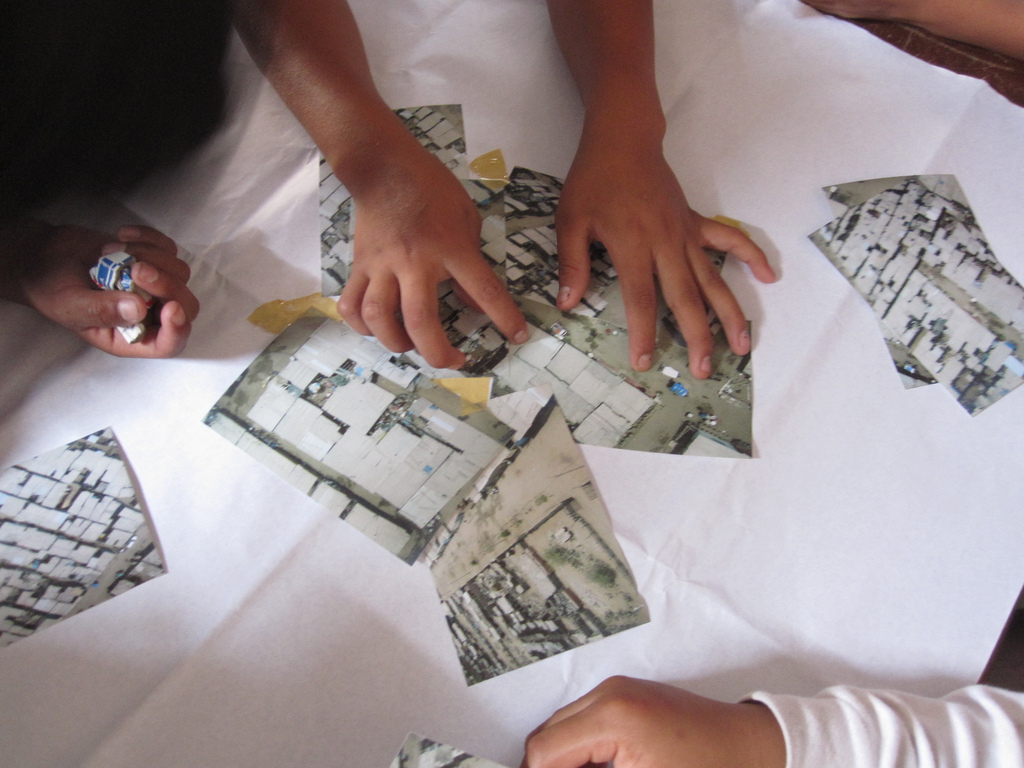
\includegraphics[width=0.45\textwidth]{images/juan-pablo-rubbersheeting.jpg}
		\caption{Students collaborate in a semi-imaginary `rubber sheeting' map stitching session.}
	\end{flushright}
\end{wrapfigure}

Most of these tools were inaccessible to the students we worked with, who were either too young or without computer access, however in order to help them understand the process we organized an activity to try to fit together printed images in a kind of puzzle, suggesting that they imagine the images printed `on rubber sheets'. This was so readily understood by all that it inspired the choice of a `rubbersheeting' interface paradigm for the Cartagen Knitter software I developed after the Lima project concluded. 

\subsection{Mapping with San Ignacio Loyola}

With Carla del Carpio, I began working with a second community called San Ignacio Loyola, approximately 1 mile southeast of Juan Pablo II. Our local partner was a teacher named Hector, who had a class of very young students, aged 5-10. Though we had limited success in mapping exercises with the class, Hector proved to be an ideal collaborator, and actively sought to internalize the skills needed to produce balloon maps, with the intention of teaching the techniques to his fall class of older students. While members of San Ignacio Loyola already have both title to their land and a completed survey of their plots, Hector saw the applicability of low-cost aerial mapping to informal settlements, and showed a lot of enthusiasm and energy in organizing flights with us despite his heavy workload as both a teacher and the community leader in charge of public works. 

Hector experienced similar if more pronounced difficulty in using Photoshop to stitch maps, but the imagery we captured with him over two 3-hour flights was superior to that of our Juan Pablo II flights. This may have been due to more favorable local wind conditions or our greater experience, but the result was a highly detailed and largely complete aerial map of the San Ignacio Loyola settlement. It became clear to us that building alliances and friendships with interested and energetic local partners was key to successful mapping.

\begin{figure}[h]
  \begin{center}
	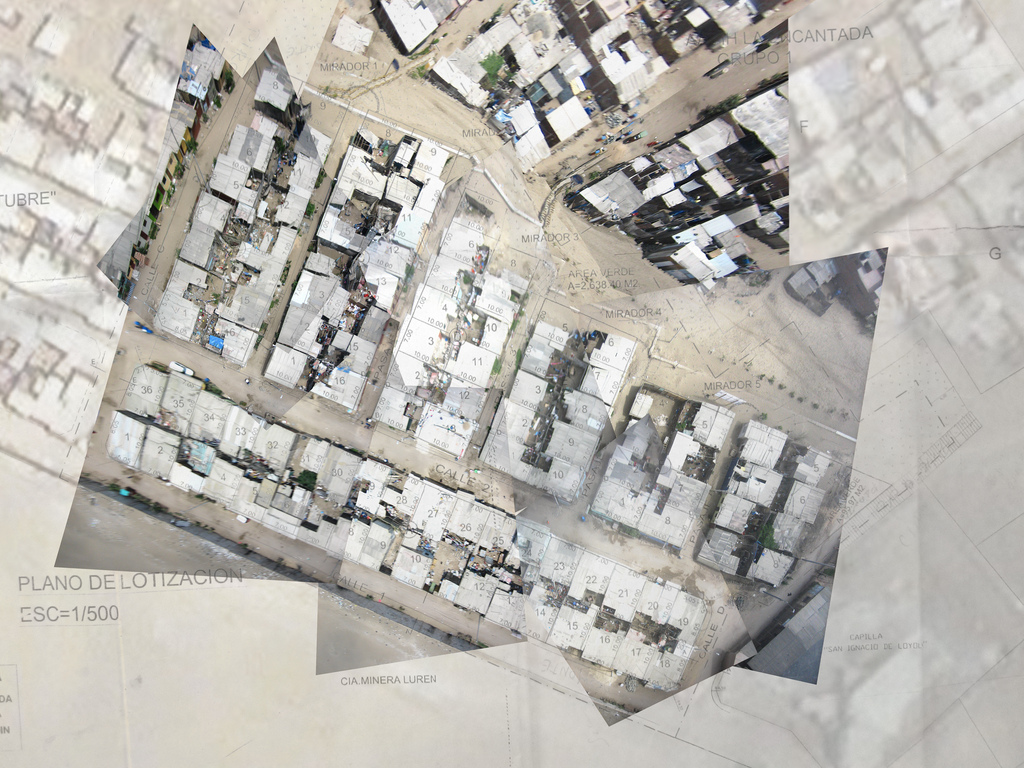
\includegraphics[width=1\textwidth]{images/san-ignacio-loyola-map.jpg}
	\caption{A balloon and kite map of San Ignacio Loyola, produced with Prof. Hector and Carla del Carpio. The map is overlaid on the existing Google Maps imagery for comparison, and also includes the surveyed plots of which Hector had a printed copy.}
  \end{center}
\end{figure}

\subsection{Mapping with Cantagallo}

It soon seemed as if `word was getting out' about our mapping efforts, as we were soon invited by Lima-based art, technology, and society foundation Escuelab, to collaborate on a mapping project with their partners in a central Lima community called Canta Gallo. Escuelab's work, led by Barcelona artist Daniel Miracle, consisted of a series of animation, filmmaking, and live television broadcasting with a Canta Gallo artist collective known as Shuawa\footnote{An interesting choice of names given that Shuawa is the name of the bird from Shipibo legend which links `maestros' in a kind of global communications network. Members of Esceulab referred to it as the `satellite bird'.}. Canta Gallo is a community of Amazonian Shipibo who have invaded a plot of land along the bank of the Rimac river; a breathtaking site in the center of metropolitan Lima. Made up of several distinct groups, the settlement comprises Shipibo and mixed heritage members who did not move to the site together, but have slowly migrated from around Lima. They have spent the last 10 years seeking legal title to the land, and different factions are at different points in the process. 

\begin{wrapfigure}{r}{0.5\textwidth}
	\begin{flushright}
		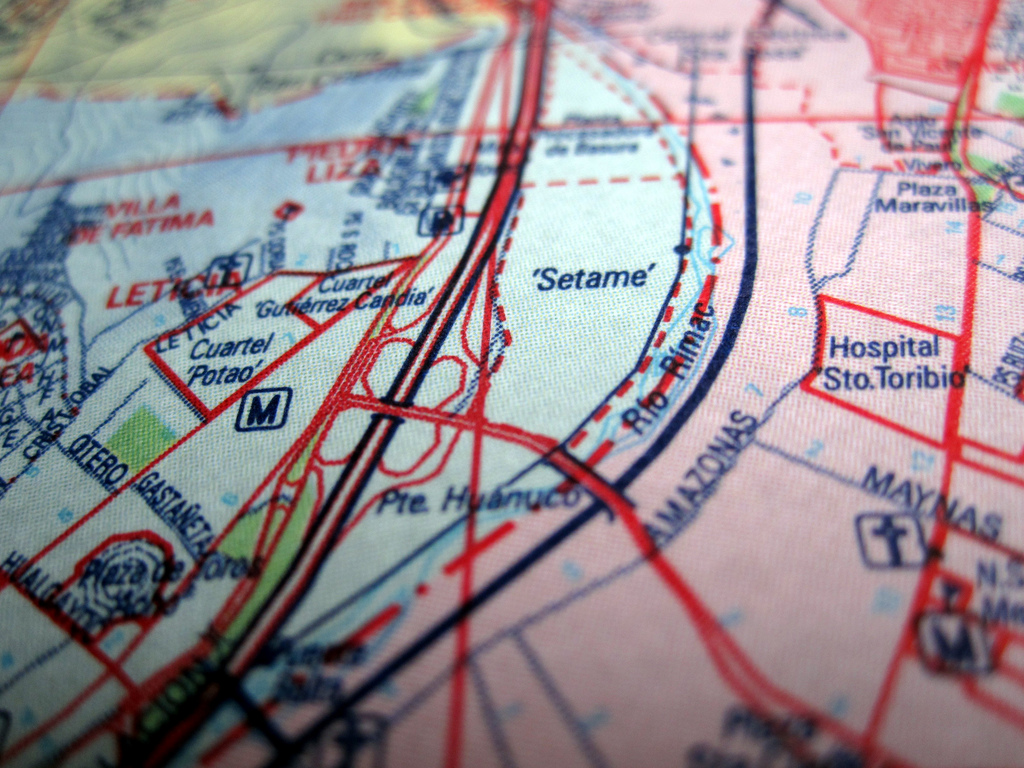
\includegraphics[width=0.45\textwidth]{images/canta-gallo-setame.jpg}
		\caption{The standard street map of Lima shows only a vacant lot owned by the city's roads administration, SETAME. The reality is a community of hundreds of people who have sought legal title for the last 10 years.} 
	\end{flushright}
\end{wrapfigure}

The group we began working with was situated on a large hill of rubble --- a landfill which leaked methane and around which residents had strewn concrete blocks to stop further dumping. Despite their difficult situation, the settlement seemed cheerful and was brightly painted with murals. An electric guitar and keyboard played in a local hangout, while posters on the communal meeting house indicated each family's dues toward land registration fees. 

In the midst of this, Escuelab had sought to establish a more neutral space by working with local artists to develop a series of arts workshops and activities for the children of Canta Gallo. Based from a state-funded school in the settlement, Daniel Miracle and others collaborated with residents such as Layner Mori to lead students in the production of digital films, animations, and incredibly, a live broadcasting news show (in the Shipibo language, no less) using a low-cost analog television transmitter. Escuelab's interests tended towards the political, as evidenced by their engagement in Shipibo/Spanish langauge issues amongst their students\footnote{The desire of some families to preserve the Shipibo language and others to raise their children with only the Castilian Spanish language was one facet of a larger ethnic division between full-blooded Shipibo and mixed-heritage members of the community. See also Zavala and Bariola's study of Cantagallo in `Enra kopiai, non kopiai: Gender, ethnicity, and language use in a Shipibo community in Lima'. \cite{bariola2008gender}}, as well as their close attention and sensitivity to the complex tenure situation and other sources of tension. However, their preference for an implicit treatment of these topics and their exploration through educational and artistic works was well matched with my own approach.

\begin{wrapfigure}{r}{0.5\textwidth}
	\begin{flushright}
		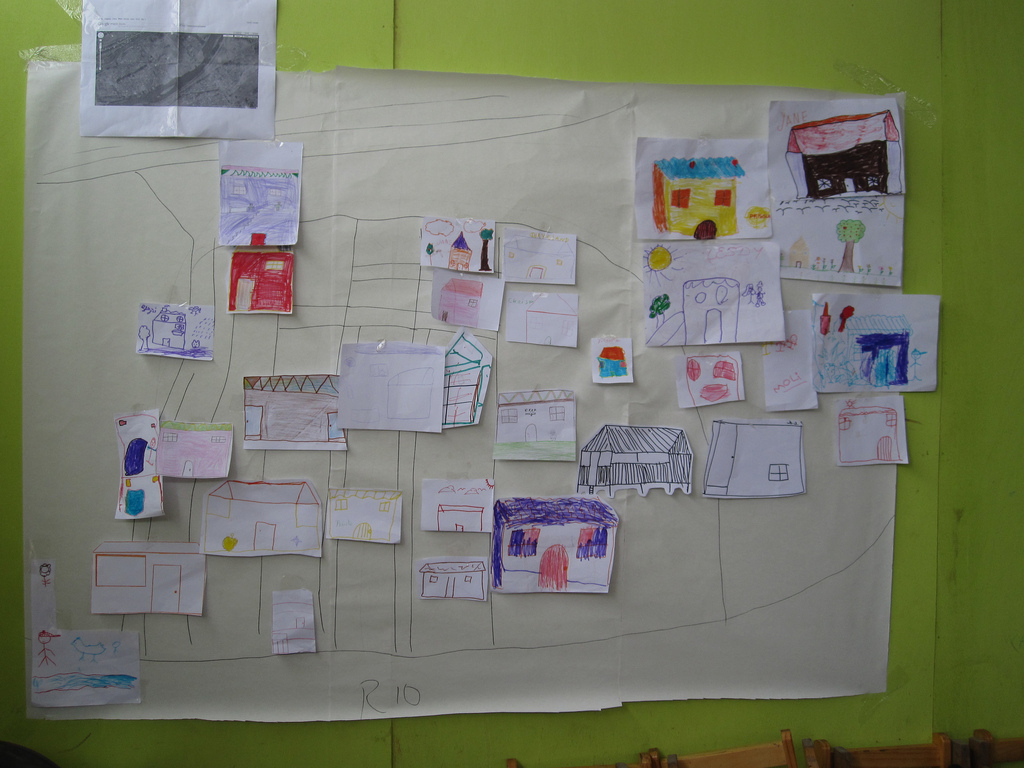
\includegraphics[width=0.45\textwidth]{images/canta-gallo-drawn-map.jpg}
		\caption{Paper map-making activities with children in Canta Gallo, Lima}
	\end{flushright}
\end{wrapfigure}

On my first day in Canta Gallo, we repeated some of the exercises I had used in Juan Pablo II, though in a shorter format. With help from Layner, we drew a large map of the settlement in rough outlines, and asked the students to draw their homes and place them on the map. The group, aged 6-12 and approximately 20 in number, produced a quantity of highly detailed drawings, though some students drew two or even three copies of their houses. One student drew one picture of his home in Canta Gallo and a second of his home in `la selva' --- presumably the home in the Amazonian region of Peru from which he had moved to Lima. While the non-literal nature of this kind of mapping presents challenges for data veracity, it is clear that children can produce a wealth of physical, historical, and culturally relevant detail, and I caution map-makers not to sacrifice this in favor of purely quantifiable information. 

\subsubsection{Flying balloons with Cantagallo}

After our sketching activities, we attempted to fly kites, as there was a light breeze. While the students were very assiduous and talented kite flyers, we eventually opted for a balloon flight, which resulted in a complete imaging of the settlement in less than two hours, from about 400 feet. To attempt a faster and more automated stitching technique, I used the open source program \textbf{hugin} and the \textbf{Autopano-SIFT} algorithm to stitch the images together, and overlaid the result on existing Google Maps imagery as well as a copy of the settlement boundaries supplied by one of the community leaders. This was our fastest time yet for the completion of a map, and was the first map --- of any kind -- of the settlement. 

\begin{figure}[h]
  \begin{center}
	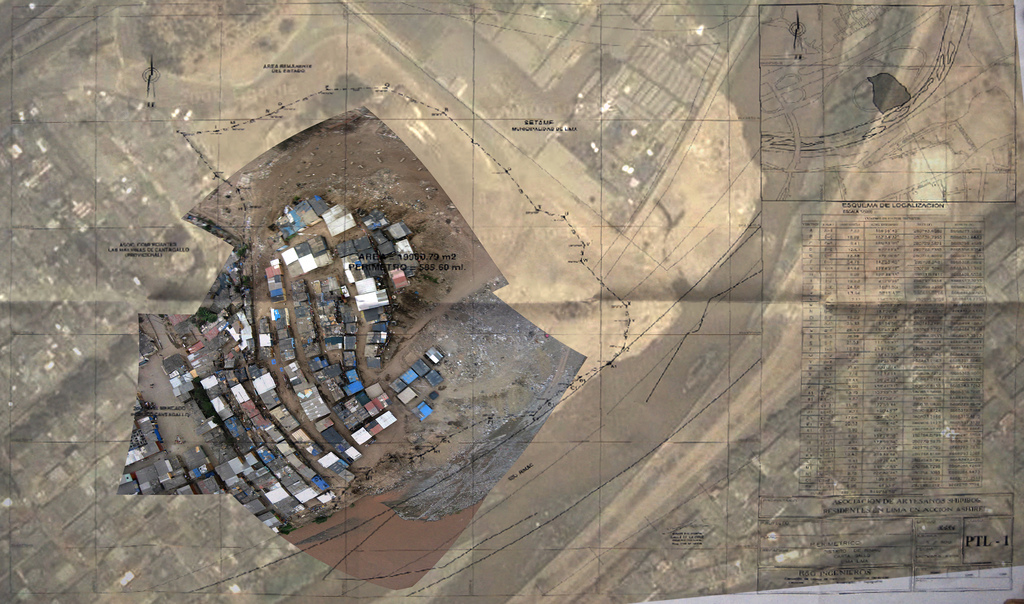
\includegraphics[width=1\textwidth]{images/cantagallo-initial.jpg}
	\caption{A balloon map of Canta Gallo, produced with Shuawa, Escuelab, and Carla del Carpio. The map is overlaid on the existing Google Maps imagery for comparison, and also includes the settlement boundaries, taken from a printed copy contributed by community leaders.}
  \end{center}
\end{figure}

\subsubsection{The rest of Canta Gallo and local geographic dispute}

Following the completion of the initial map of Canta Gallo, Sara Gomez of CEDRO suggested that we attempt to map the adjacent settlement, which I was surprised to find was also part of Canta Gallo. Collaborating again with Daniel Miracle and Escuelab, we met with Sr. Ricardo, the leader of the lower part of Canta Gallo and spent a day mapping that area as well. I worked with Layner Mori using Photoshop to stitch the resulting imagery over a map supplied by Sr. Ricardo, and we printed a paper copy. In a discussion with Sara, Layner, and Daniel, we decided to combine the two maps --- which showed some overlap -- and distribute the combined map. 

\begin{figure}[h]
  \begin{center}
	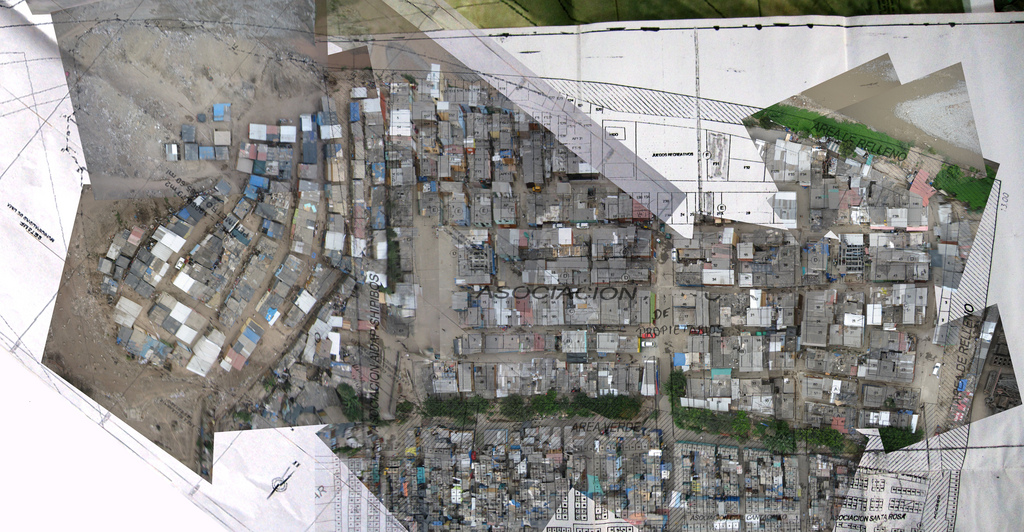
\includegraphics[width=1\textwidth]{images/cantagallo-combined.jpg}
	\caption{A balloon kite map of all of Canta Gallo, produced with Shuawa, Escuelab, Sara Gomez, Carla del Carpio, and residents of Canta Gallo. The map is overlaid on the existing Google Maps imagery for comparison, and also includes printed maps contributed by community leaders. Note that a small area is missing; unfortunately the balloons popped near the end of the day and we lacked enough helium to continue.}
  \end{center}
\end{figure}

Producing a combined map was a potentially controversial decision, as the two settlements were experiencing some tension due to both ethnic and territorial issues. The lower settlement, spread over a much flatter and larger area, was presumably further advanced in its bid for land title, as they had a surveyed map with well-defined plots, whereas the upper settlement with whom we had first worked had only a map of its outer boundaries. However, in an attempt to avoid involving ourselves in local political issues, we deemed it more fair to provide maps and mapping tools to both communities equally. In retrospect, I feel that to attempt to position ourselves as neutral parties may have been misguided, as producing maps and teaching map-making workshops are by no means a neutral acts. However, I do believe that providing open access to these tools and techniques, as well as to the geographic information they can produce, is a positive goal. One aspect of maps which I value highly is their ability to reconcile differing mental models of a geography, and to make explicit the differences between those models. My hope is that we helped to do so in an inclusive manner. 

\begin{table}[tp] 
\caption{Comparison of maps produced in January 2010 project in Lima, Peru with those available in Google Maps for same period.} 

\label{fig:limaevaltable}\centering %
\rowcolors{1}{tableShade}{white}
\renewcommand{\arraystretch}{1.4}
\begin{tabularx}{\textwidth}{>{\bfseries}rlYYY}
\toprule\hiderowcolors
Site&Criteria&Grassroots Mapping&Google Maps&Percent change\\\otoprule\showrowcolors
Juan Pablo II&Resolution&29cm&4.4cm&+659\\
&Recency&new&2-3 yrs old&\\\hline
San Ignacio Loyola&Resolution&29cm&3.4cm&+853\\
&Recency&new&2-3 yrs old&\\
&Roof count&&&\\\hline
Canta Gallo&Resolution&29cm&7cm&+411\%\\
&Recency&new&2-3 yrs old&\\\hline
\bottomrule
\end{tabularx}
\end{table}

\subsection{Evaluation}

Any comprehensive evaluation of the map-making work I and my local partners performed would need to include a long-term examination of the maps' uses; legal, urban planning, educational, and political applications were among our hopes, but many of these processes occur on a timeline of years or even decades. Still, in the half year since their creation, the maps of Canta Gallo have been used for subsequent projects by Shuawa, and Helder Solari, one of the activists involved in the original map-making, asserts that `in fact even now there is none better than yours. In other maps Canta Gallo simply doesn't exist.' While I look forward to hearing of as well as advocating further uses of these maps, the immediate evaluation I can attempt will have to rely upon the maps' reception among participating community members and in the qualitative and quantitative measures which can be made today.

(Cite Remote Sensing table)

On a resolution basis, these maps are far superior to any which have been made before (see Figure \ref{fig:limaevaltable}). However their most important quantitative advantage is in their recency; in comparison, those available on Google Maps are hopelessly obsolete, sometimes showing only a small percentage of the buildings which exist today. Due to these impressive numbers, a variety of individuals and organizations have suggested uses for the data, ranging from tracing and import into OpenStreetMap to use in World Bank needs assessment or municipal datasets. While I think these are generally good ideas, I also believe that the decision to publish any map data is one which community leaders and those involved in the creation of the data should make. My own publication of these maps for educational and research use was only after explicit permission was granted by all involved parties. 

\begin{figure}[h]
  \begin{center}
	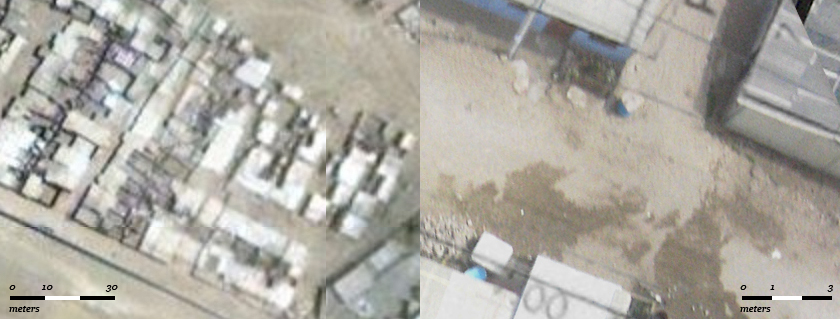
\includegraphics[width=1\textwidth]{diagrams/san-ignacio-scale.jpg}
	\caption{Comparison of scales and level of detail between Grassroots Mapping imagery and existing Google Maps/GeoEye imagery.}
  \end{center}
\end{figure}

Finally, and far more importantly than the technical evaluation, I was careful to record the reception and discussion of this project amongst its participants, and especially amongst the residents of the areas we mapped.\footnote{For a more thorough discussion of my evaluation strategy, see Section \ref{sec:lather}.} This took the form of informal interviews with partner organizations and residents, as well as my notes and observations, but due to the extremely speculative nature of the project, it followed no specific plan. I want to be clear that this is by no means an attempt to develop a formal scientific or ethnographic study. Rather, it represents the information with which I developed a more comprehensive and measured approach in subsequent case studies.   

- Interviews!!!!!!! transcribe them



\subsection{Needs (Re)assessment}

The Lima project demonstrated the feasibility of participatory map-making projects with low cost tools such as balloons and kites. However, it also highlighted the need for a simplification of available tools and for new, easier interfaces, especially for the digital post-processing steps, in order to increase inclusion and avoid dependency on outside assistance. Specifically, the orthorectification and publication tools we tested were inadequate and the feedback and brainstorming we conducted with various collaborators led me to begin planning a new tool, one which eventually became the Cartagen Knitter discussed in Section \ref{subsubsec:knitter}. This tool would need to be easy to install, or run in any internet cafe (I opted to make run in a web browser). It would need to make use of an intuitive mental model for orthorectification; rubber sheeting, as explored with students from Juan Pablo II, was a good fit. It would need to export in a format which could be easily printed, and finally, it would need to be tested in the field with a diverse group of users. 

On the hardware side, the difficulties we experienced in flying balloons and kites in Juan Pablo II emphasized the importance of good equipment, timing, and a good understanding of local weather conditions. Still, the exceptional maps we were able to produce at every site were encouraging, and the speed with which we were able to map a given site suggested that repeated periodic mapping, or mapping much larger areas, could be possible. 

Above all, I learned the importance of building capacity amongst local partners, and of taking seriously the pedagogical challenges of this kind of participatory map-making. My experiences teaching others to use these tools, and working with them to adopt, internalize, and improve the necessary techniques to create maps, emphasized the need for better teaching materials, guides, and a more structured approach to skills transfer. These would be major themes in the following case study in the Gulf of Mexico, where many of the lessons learned in Lima were put to the test. 

\chapter{Case Study: Citizen mapping of the BP oil spill}
\label{chap:gulf}

\section{Grassroots mapping in crisis response}

In late April 2010, the Deepwater Horizon oil rig exploded and sank, initiating what may be one of the worst environmental disasters in US history. As the spill grew in size, I contacted Stewart Long of GonzoEarth.org and Oliver Yeh of 1337arts.com. \begin{wrapfigure}{r}{0.5\textwidth}
	\begin{flushright}
		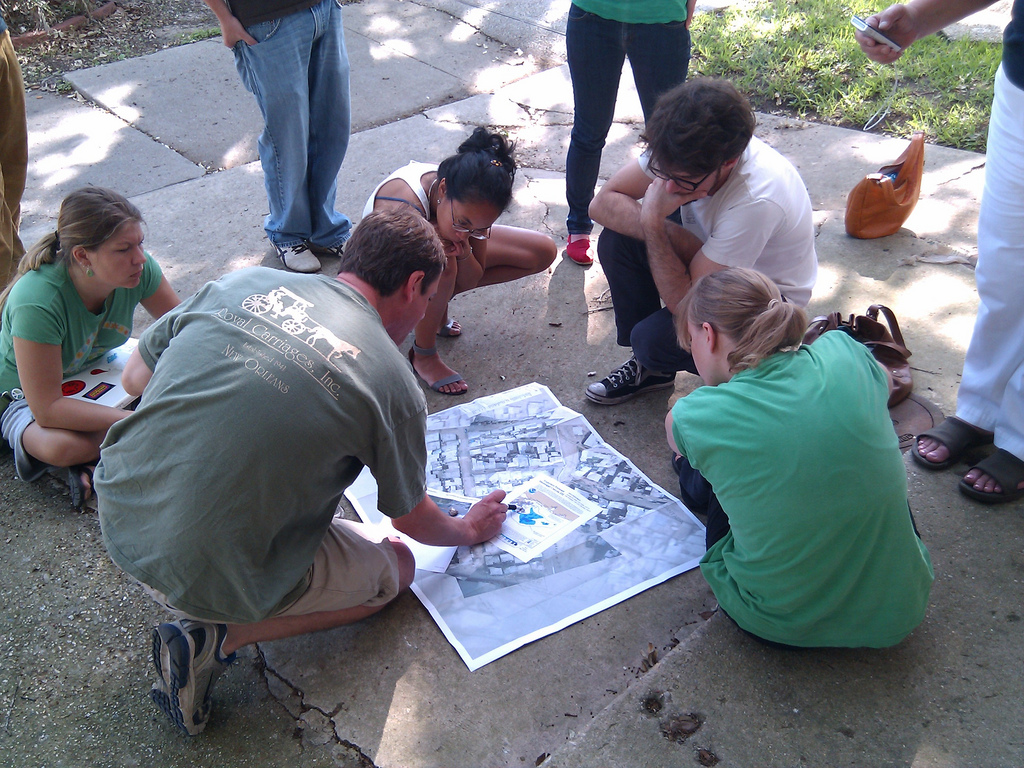
\includegraphics[width=0.45\textwidth]{images/labb-planning.jpg}
		\caption{Volunteers at the Louisiana Bucket Brigade in New Orleans plan a mapping trip on May 7, 2010.}
	\end{flushright}
\end{wrapfigure}Long has used remote control aircraft to produce maps, and Yeh specializes in high-altitude photography using weather balloons, having captured imagery from a balloon at altitudes of over 90,000 feet. The three decided to travel to the Gulf Coast area to spearhead a citizen effort to map the oil spill's effects. After making phone contact with Anne Rolfes of the Louisiana Bucket Brigade (LABB), a New Orleans-based environmental activist group, Yeh and I flew to New Orleans on May 5th 2010, followed by Long on May 6th. 
% env. crisis in US history: http://www.npr.org/templates/story/story.php?storyId=126410895
% http://www.nytimes.com/2010/04/25/us/25rig.html - Oil Leaking Underwater From Well in Rig Blast, By CAMPBELL ROBERTSON, April 24, 2010

With the cooperation and extensive support of the LABB and other interested New Orleans residents, the team began leading almost daily trips to use balloons and kites to map coastal areas. While not attempting to produce imagery of the entire at-risk coastline, which stretches several thousand miles from Louisiana to Florida, the mappers focused on acquiring high resolution imagery of specific sites, with the goal of producing 'before and after' maps. The trips relied on the availability of free transport to affected areas, but in the initial days of the project this was not a problem, as fishermen and charter companies began calling in to offer their services for free. Increasingly large areas of the Gulf of Mexico were being closed to fishing, and with their livelihoods at risk, many in the fishing industry were eager to participate in the documentation of the spill. 

% fishery closings: http://sero.nmfs.noaa.gov/deepwater_horizon_oil_spill.htm 

\section{Comparing Grassroots Maps of the spill to other sources}

The 2010 Gulf oil spill was seen as an opportunity to apply the low-cost mapping techniques refined and documented on GrassrootsMapping.org to a problem of immediate import. While many overflights were occurring, there was no publicly available, orthorectified imagery available in the initial weeks of the spill; up-to-date imagery was supplied mainly by the MODIS (Moderate Resolution Imaging Spectroradiometer) sensors aboard NASA's Terra and Aqua satellites.\footnote{Since then, overflights by } MODIS is limited to 1000 meter resolution for those bands which are used for ocean imaging, and while the daily images available were very useful in determining where along the coast was being hit by slicks and sheens, it was not of high enough detail to show any specific damage. 

% http://modis.gsfc.nasa.gov/about/specifications.php
\begin{figure}[h]
  \begin{center}
	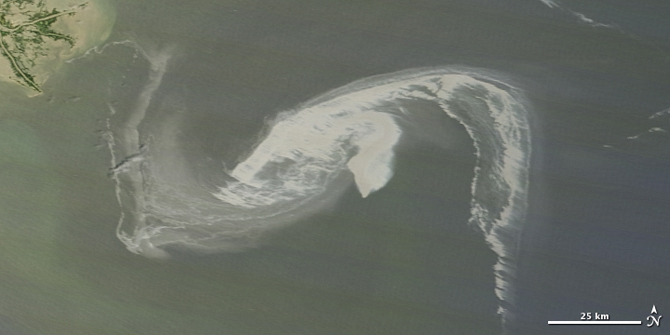
\includegraphics[width=1\textwidth]{images/nasa-modis-small.jpg}
	\caption{The BP oil spill on April 29th, 2010. The upper left corner shows the tip of Louisiana. Imagery from NASA's Terra satellite, using the MODIS sensor.}
  \end{center}
\end{figure}

By contrast, the imagery collected by the LABB/Grassroots Mapping teams was up to 9 cm/px in resolution, and could be repeatedly captured over the course of days or weeks. In addition, the unfolding nature of the oil spill crisis made it important to visit and map sites both before and after oil was sighted, and periodically afterwards. The potential for a set of maps of the same site, taken at intervals, to depict progressive damage to ecosystems and economies is a powerful new dimension to the project.

(Cite Remote Sensing table and wetlands paper, miyamoto)

\section{Independent monitoring and media blackout}

As the crisis progressed, it became clear that BP was attempting to restrict access to affected areas by means of airspace restrictions, closing public beaches, and preventing boats from entering some areas. The Breton Sound was closed to the public in mid May, and flyovers were restricted to a minimum of 4,000 feet, making it difficult to photograph or identify features on the ground. \cite{peters2010efforts} With reduced public and media access, many became concerned that because of the close collaboration between BP, the Coast Guard, and NOAA, the government was becoming complicit in the media blackout. Even on the ground \ac{LABB} mappers found that many cleanup workers were prohibited from talking about what they were doing. \cite{labb2010heywhat} This gave our mapping effort new meaning, as our imagery was among the best available for many areas, and the support we received from local fishermen in getting to sites helped us to sidestep issues of access which limited many in the mainstream press.

\section{Sustainability}

\begin{wrapfigure}{r}{0.5\textwidth}
	\begin{flushright}
		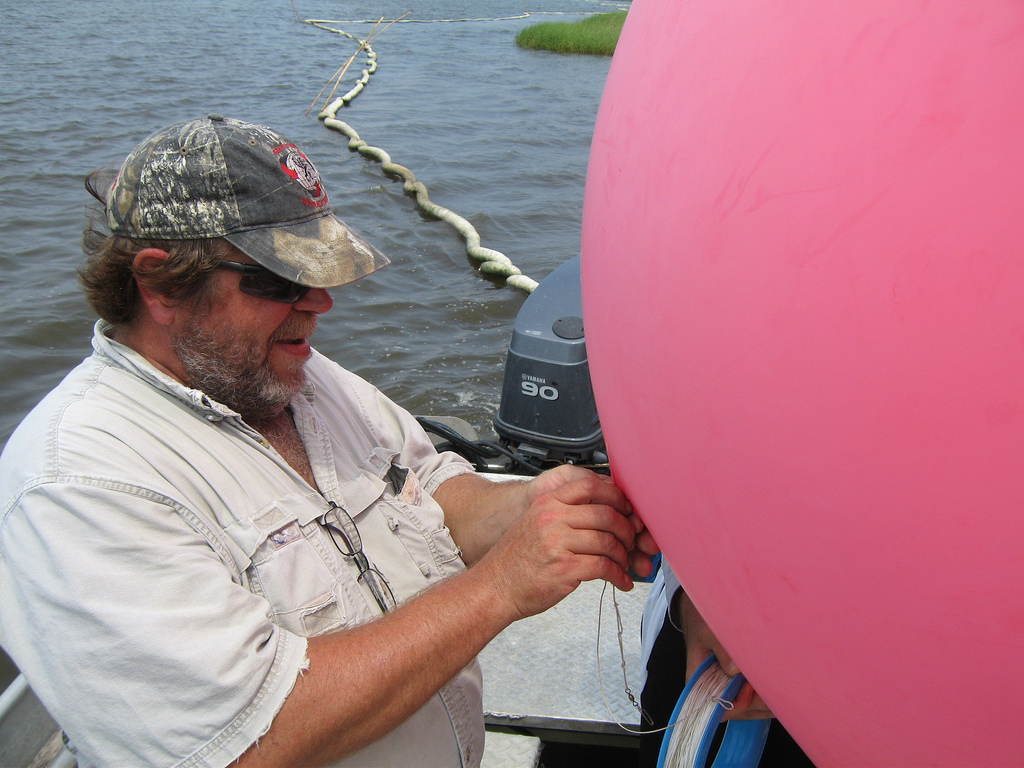
\includegraphics[width=0.45\textwidth]{images/labb-bay-babtiste-trip.jpg}
		\caption{A volunteer prepares a balloon for launch in Bay Babtiste, Louisiana, July 11, 2010. Photo courtesy Flickr user \textbf{guiltyplanet}, at \url{http://www.flickr.com/photos/guiltyplanet/4784059359/}}
	\end{flushright}
\end{wrapfigure}

The most challenging aspect of organizing the oil mapping project was to train a group of inexperienced but committed volunteers to use Grassroots Mapping tools such as balloons and kites, in often adverse weather conditions up to 3 hours travel from New Orleans, our home base. That a number of volunteers have continued not only to make trips on their own, but to bring and train others to map, has been both exciting and impressive.

Between May 7th and July 22nd, over 47 participants made 36 trips to gather mapping data, or almost one every other day. While only one trip has failed to return with imagery, 56\% of trips returned with `excellent' or `useable' data, indicating that some quality control mechanisms might result in a higher success rate. Still, over 11,000 images have been taken, with plans and funding in place to continue mapping through January 2011. 

(Get Adam Griffith's photo from the 2 days grand isle post)

\begin{wrapfigure}{r}{0.5\textwidth}
	\begin{flushright}
		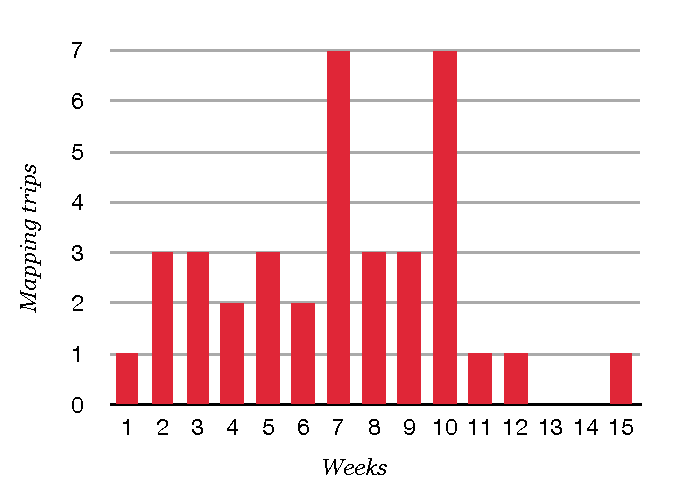
\includegraphics[width=0.45\textwidth]{diagrams/mapping-trips.pdf}
		\caption{Number of mapping trips per week. Drop in trips starting in week 11 was due to high summer heat and the absence of several of the project's main trip leaders who were on vacation.}
	\end{flushright}
\end{wrapfigure}

\subsection{Workshops and trainings}

One factor that likely played a major role in the rapid adoption of Grassroots Mapping techniques was the early emphasis on training. With \ac{LABB}, we organized a workshop in the first week of mapping for potential volunteers, where we demonstrated the use of the tools in a hands-on manner, flying kites and capturing a sample data set. In addition, trips to mapping sites have continued to attract new volunteers, and the teaching of aerial mapping techniques to newcomers has been a priority throughout the project. We have been lucky that \ac{LABB} has combined their outreach programming with aerial mapping trips, resulting in a steady flow of new mappers. 
As shown in Figure \ref{fig:tripspermapper}, while a large body of participants  .

...

\begin{wrapfigure}{r}{0.5\textwidth}
	\label{fig:tripspermapper}
	\begin{flushright}
		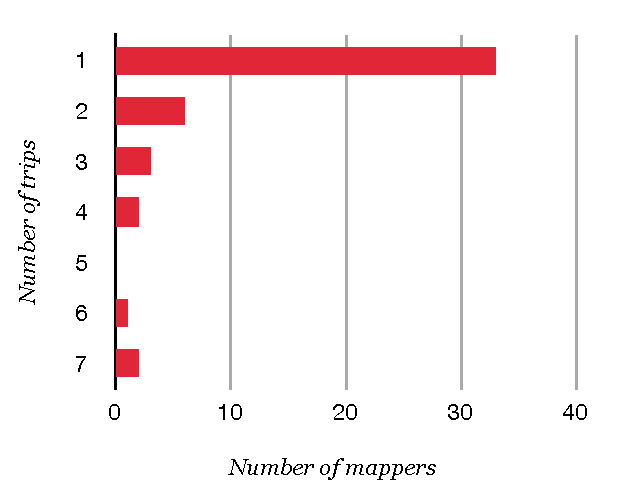
\includegraphics[width=0.45\textwidth]{diagrams/mappers-histogram.pdf}
		\caption{Number of mapping trips per mapper}
	\end{flushright}
\end{wrapfigure}

Particularly encouraging was the participation of two mappers who had seen just a single presentation about the project, and were inspired to begin balloon mapping on their own. Assembling their own kit based on information available on the Grassroots Mapping website, Don and Justin Blancher contacted us with hundreds of photos of Perdido Point, Alabama. Delighted, we arranged a transfer of files and Stewart Long created a map within a few days. The two continue to contribute new data.  

\subsection{Collaborations}

From the start of the project, the Grassroots Mapping mailing list and wiki were a focal point for collaboration, and members of the wider Grassroots Mapping community helped identify local helium sources, coordinate volunteers, and even paid for plane tickets. On the ground, there was also considerable ad-hoc collaboration, with Oliver Yeh of 1337arts and Stewart Long of GonzoEarth leading trips and trainings on multiple occasions. However, over the first several weeks, Shannon Dosemagen of the Louisiana Bucket Brigade, and Kris Ansin of the University of Tulane's School of Public Health and Tropical Medicine emerged as leaders of local mapping trips, and their efforts have ensured that map-making has continued for close to three months since our initial efforts. Long and myself played a supporting technical role in managing, processing, and publishing stitched maps of the data, and advising the LABB team on equipment setup and maintenance. 

Throughout the project, we made parterships with a variety of other organizastions to share boat trips, imagery, and to collaborate directly on capturing imagery --- among these were the Blue Seals, Greenpeace, Americorps, and many individuals who volunteered their time, money and abilities. This dense web of collaborations has formed a backbone of support for the effort, and ensured its regularity and sustainability. While the urgency of the disaster itself surely played a role in forging such a network of mutual support, such strong local participation must be an integral part of \textbf{any} participatory mapping effort which expects to be sustained beyond an initial burst of enthusiasm.

\subsection{Funding model}

Mapping the spill incurred a range of new costs; not only is there a virtually unlimited potential area to map, but the intention to repeatedly map each site meant that there is no completion criterion for the effort --- trips are led and imagery is captured as often as possible given the constraints of time and money. While the costs of equipment were still in the range of \$150-200 per kit, travel turned out to be the most expensive part of the project. Not counting the hours of donated time and associated fuel costs on boats, planes, and in cars, a typical day in a chartered boat cost approximately \$US 400, and even teams visiting only the shoreline had to travel for upwards of 3 hours each way from \ac{LABB} headquarters in New Orleans. 

Various donors and institutions were generous in their support of the project, including the Center for Future Civic Media, the Lafourche Port Commission, the Washington Post, Development Seed, and many more.\footnote{For a full list of donors please see Appendix \ref{app:donors}} In order to meet these expenses, on May 29th I created a proposal at \href{http://kickstarter.com}{Kickstarter.com} with help from filmmaker Kristian Hansen. Kickstarter is a site where individuals can elect to `back' a project financially, receiving rewards for different levels of support. For \$50, we offered to put backers' names on a balloon, for \$1000, we promised to send backers a complete Grassroots Mapping Kit. However, the vast majority of donations were at the \$25 level, and a total of 145 contributors backed the project with \$8,285 by June 21, 2010.

Funding the project in this manner rather than via larger institutional grants seemed appropriate for an already citizen-led, independent effort to document the oil spill's effects. For many, contributing a small amount or even simply spreading the word was the only means of participating. For these reasons the choice of Kickstarter as a means to financial sustainability is especially relevant to the project's mission. 

\section{Image processing and map stitching}

Throughout the project in the Gulf of Mexico we have relied heavily on Adobe Photoshop for manual orthorectification of maps, due to its proven track record and known limitations. Other tools such as Map Warper and Cartagen Knitter were limited by their dependence on OpenStreetMap base data, though Cartagen Knitter has since gained the ability to display a base layer of tiled satellite imagery, and may see increased usage for future map data sets. Photoshop produced \ac{TIFF} images which were processed into \ac{GeoTIFF} and cut into tiles using the \textbf{gdal2tiles.py} script. This generated both a \ac{TMS} and a \ac{KML} for viewing online. Maps were also uploaded to Flickr for public viewing, though at a lower resolution, since Flickr limits uploaded files to 10 megabytes in size. In addition, the most permissive license provided by Flickr was Creative Commons Attribution, so maps were annotated as Public Domain data in each image's description field. 

Those in the project who were able to produce stitched maps, including myself and Stewart Long with some help from David Riallant and Cesar Harada, were challenged to keep up with the fast pace of map data submission. New data sets arrived as often as every other day, and a single set typically included hundreds of images to be sorted, processed for brightness and contrast, and stitched. A large monitor and a powerful computer were required, and even my own 8-core 3 GHz workstation took up to 10 minutes for each transform on larger maps. These issues, as well as the difficulty in including a broader group in the stitching effort, highlighted the need for a completed Cartagen Knitter tool, even as it took time away from its development. 

\begin{wrapfigure}{r}{0.5\textwidth}
	\begin{flushright}
		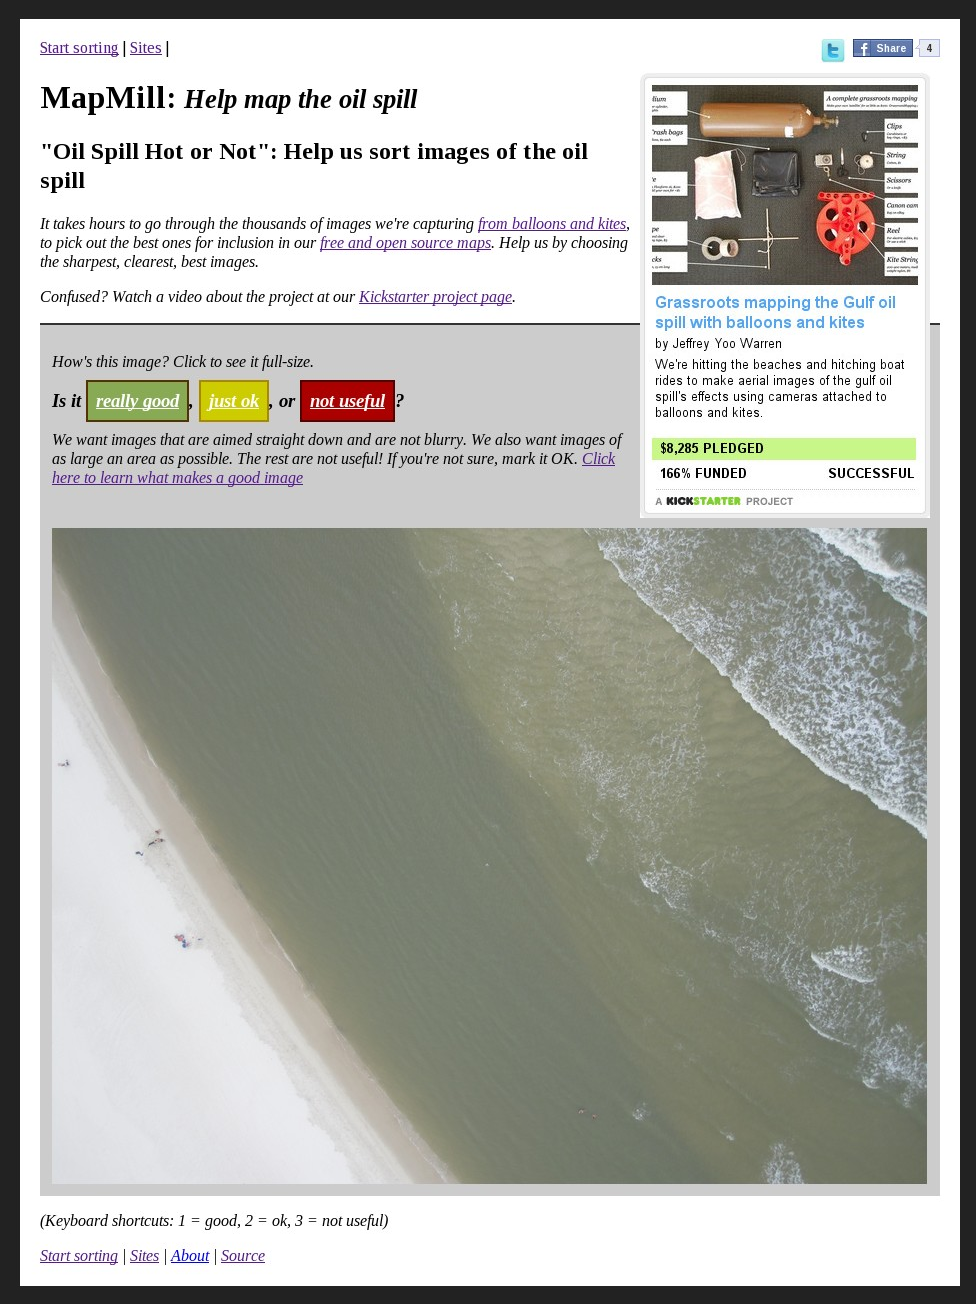
\includegraphics[width=0.45\textwidth]{images/mapmill.png}
		\caption{MapMill.org image sorting website developed in response to the high-volume data submission from the Gulf of Mexico during the BP oil spill.}
	\end{flushright}
\end{wrapfigure}

One tool I developed in response to this overwhelming amount of data was called MapMill, available at \href{http://mapmill.org}{mapmill.org}. As sorting through images often took a substantial amount of time before orthorectification or stitching could begin, visitors of MapMill were presented with an aerial image, and asked to rank it as `really good', `just ok' or `not useful' in an adaptation of the interface to the well-known `HotOrNot' website. A one-page visual guide was offered to demonstrate what constitutes a `good' image, highlighting crispness, good exposure and downward-facing camera angle. In the 50 days following its launch on June 16th, 2010, images have been ranked more than 23,000 times, demonstrating that a voluntarily crowdsourced means of image processing may be feasible. 

\section{Integration with Ushahidi}

The \ac{LABB} team had already set up an instance of the Ushahidi mobile-phone based crisis reporting tool for crowdsourced information gathering, and this continues to be one of their main priorities and most publicly visible responses to the spill. To better integrate our aerial mapping data with the Ushahidi platform, I inserted \ac{TMS} layers of our data into the OpenLayers-based Ushahidi map display, so that report locations would appear overlaid on aerial imagery where available. This generated a feedback loop for mappers, who would often look to Ushahidi to identify clusters of oil sightings which made good candidate sites for aerial mapping.

\begin{wrapfigure}{r}{0.5\textwidth}
	\begin{flushright}
		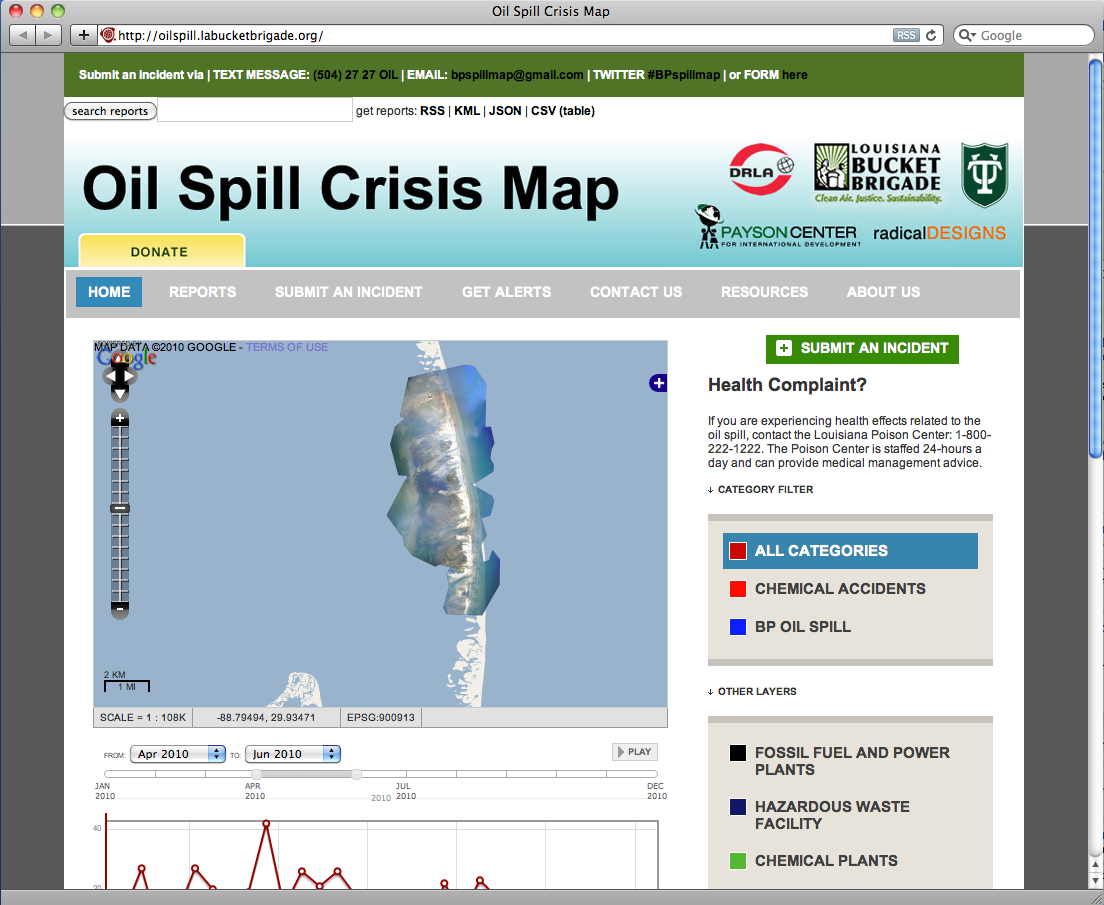
\includegraphics[width=0.45\textwidth]{images/labb-ushahidi.png}
		\caption{Data collected and processed by the Grassroots Mapping team, displayed as tiles in the LABB Ushahidi instance.}
	\end{flushright}
\end{wrapfigure}

\section{Overflights and a broader data strategy}

As more organizations such as the Blue Seals and the Louisiana Environmental Action Network became involved, opportunities arose for the capture of data from donated airplane flights. While this was outside the scope of the Grassroos Mapping Kit, we took every opportunity to gather such data, and several of the datasets we have published were captured by volunteers on such flights, or were donated and released into the public domain. This has helped make a connection in scale, methodology, and image quality between our balloon and kite derived imagery and more conventional techniques, and in retrospect may help those in crisis management situate our work in a larger data gathering strategy. 

\section{Documentation}

The disaster and the incredible support and diligence of the LABB mapping team also generated a wealth of both qualitative and quantitative information on the volunteer-led effort to apply Grassroots Mapping tools toward the collection of crisis information. Mapping team leaders filled out a form describing a variety of information from weather conditions at the site to the condition and performance of the gear. Leaders built deep experience in gathering data and teaching others, and many wrote blog entries or spoke to the press about their experiences. Beyond serving as a valuable independent record of the spill, this case study lays solid groundwork for the application of these tools to other environmental, social, and political crises.

\section{Analysis of data collected}

New imagery continues to arrive from mapping trips across the Gulf Coast, but the data we have so far is useful for examining what factors affect the success rate of mapping attempts, as well as to assess the increase in data quality as participants gain experience and the techniques mature. Of course, it is also of interest to quantify our results to date in terms of resolution, extent, and fidelity.  



overall success rate 

what works and doesn't

correlations between experience and success in trips

(days or weeks to process - need for Knitter)

\begin{wrapfigure}{r}{0.5\textwidth}
	\begin{flushright}
		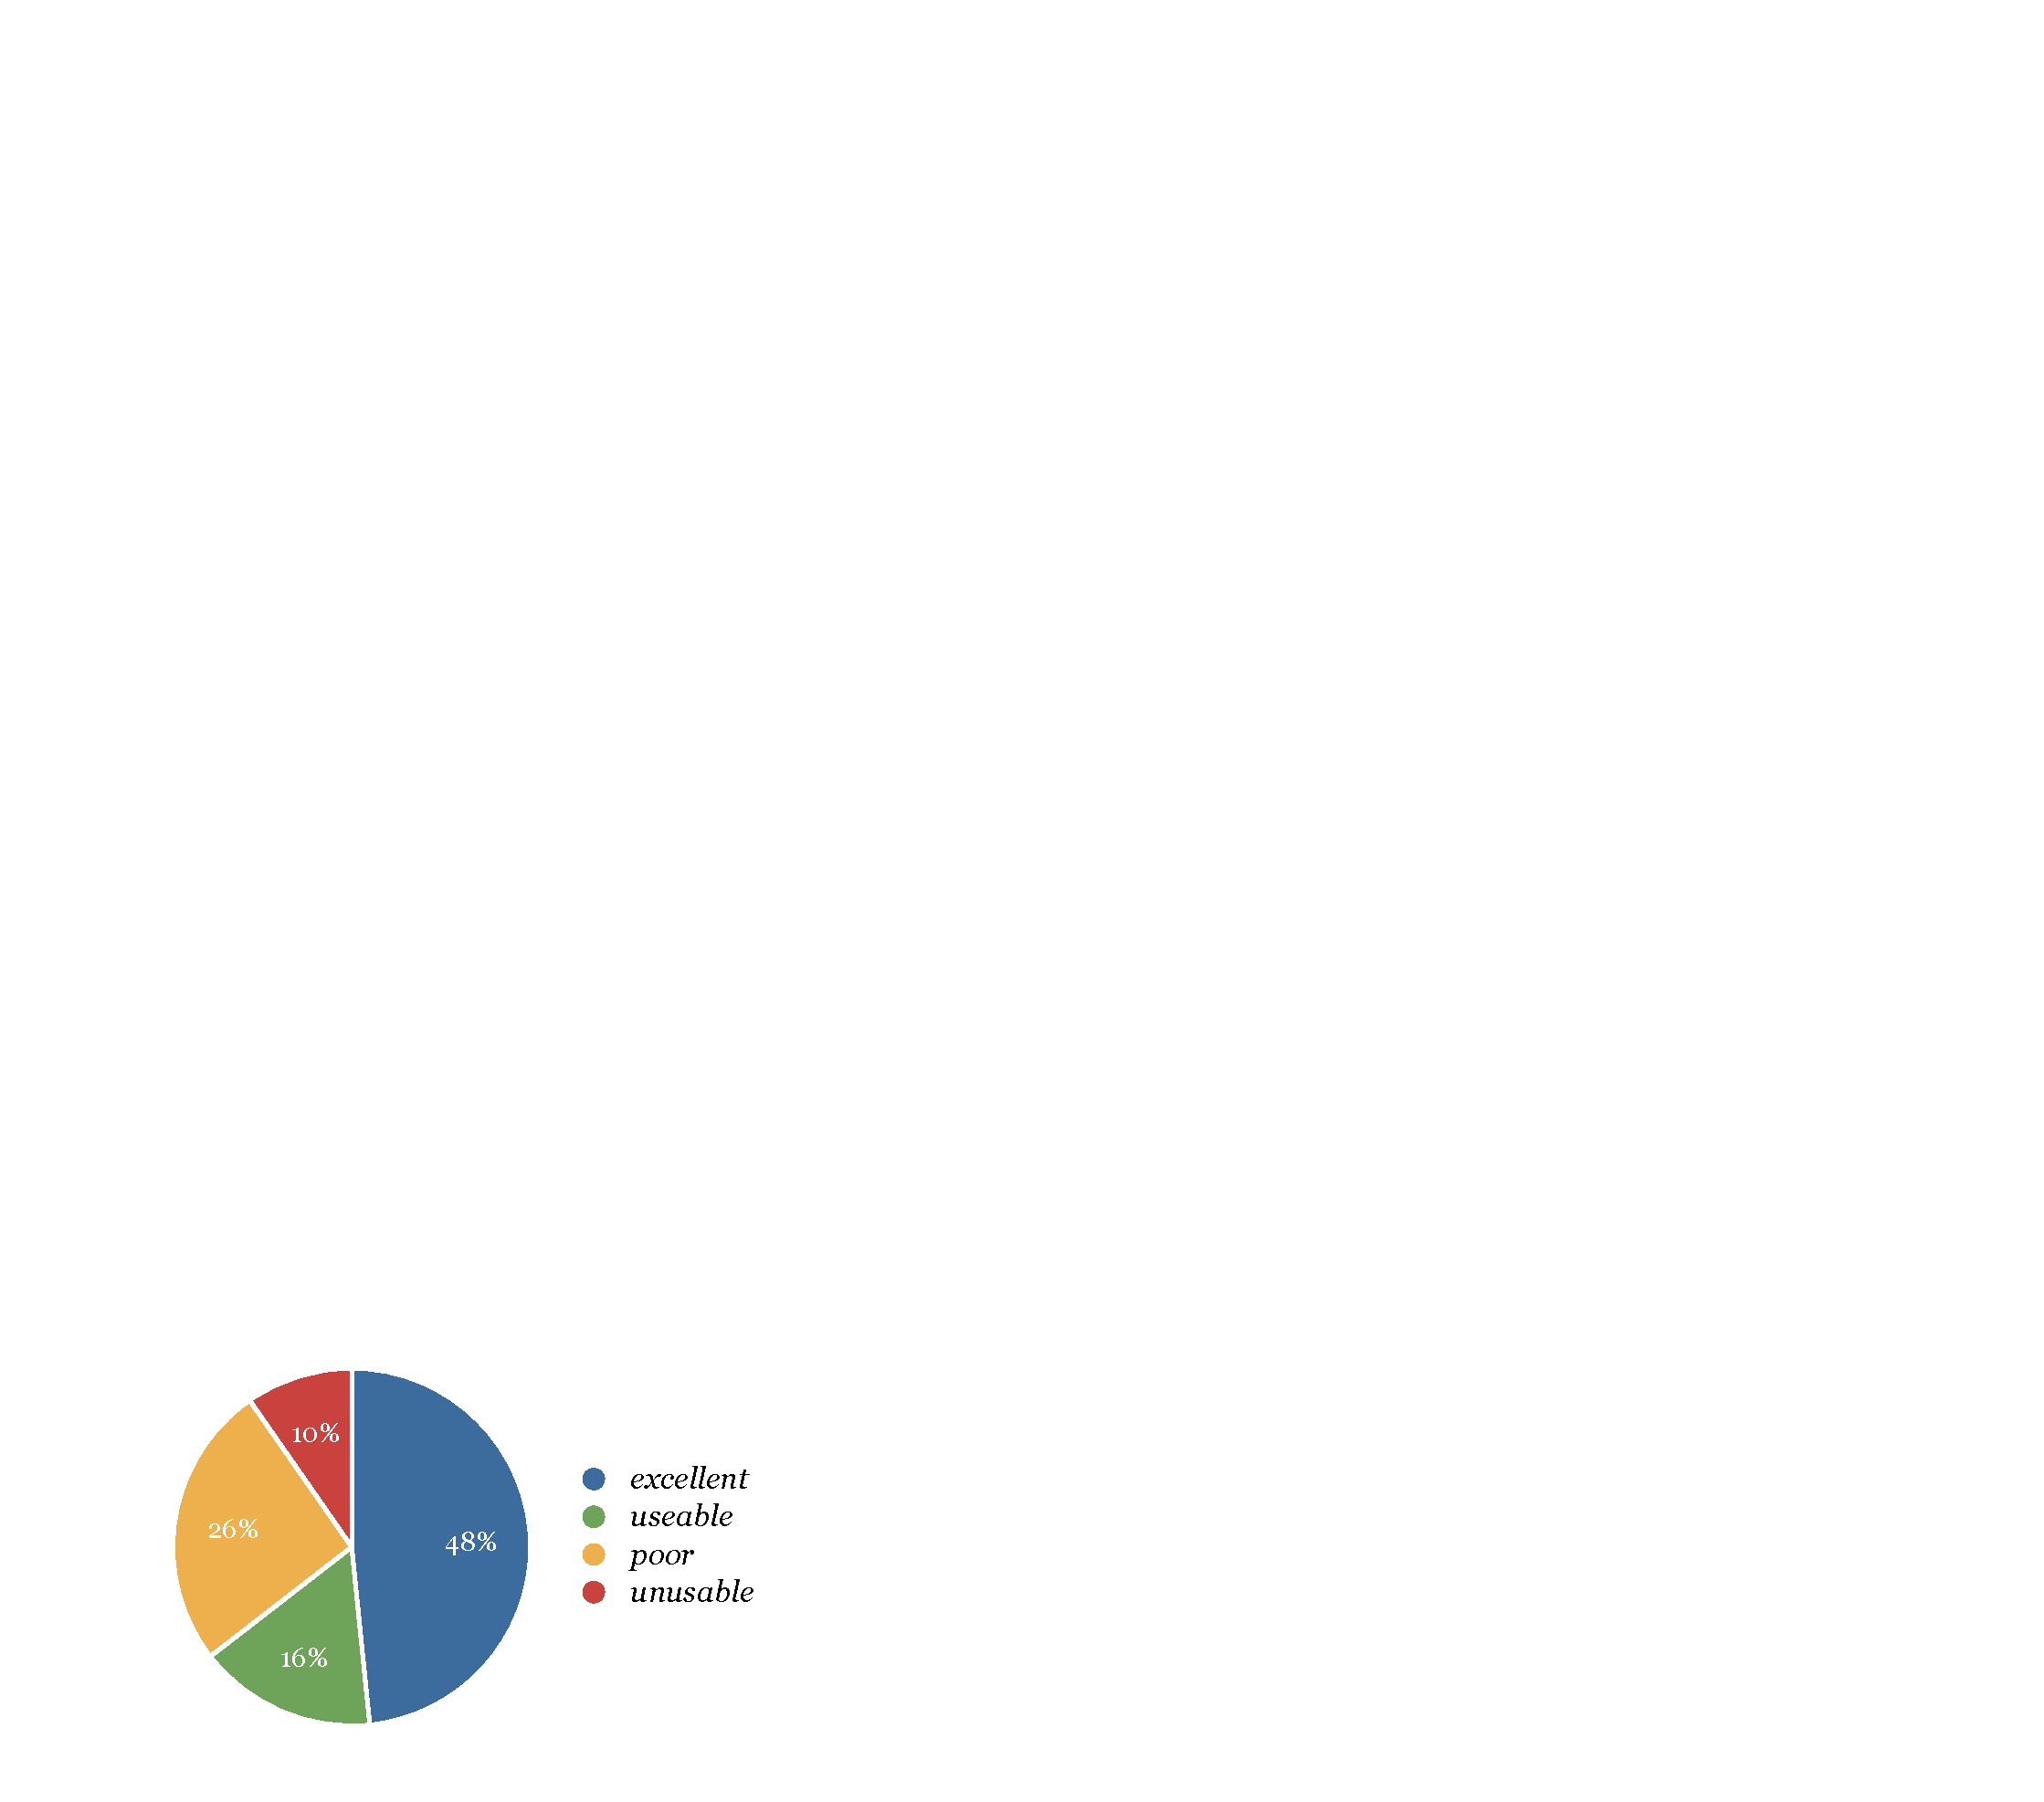
\includegraphics[width=0.45\textwidth]{diagrams/gulf-trip-success.pdf}
		\caption{Success of mapping trips, based on number of images captured}
	\end{flushright}
\end{wrapfigure}


\begin{wrapfigure}{r}{0.5\textwidth}
	\begin{flushright}
		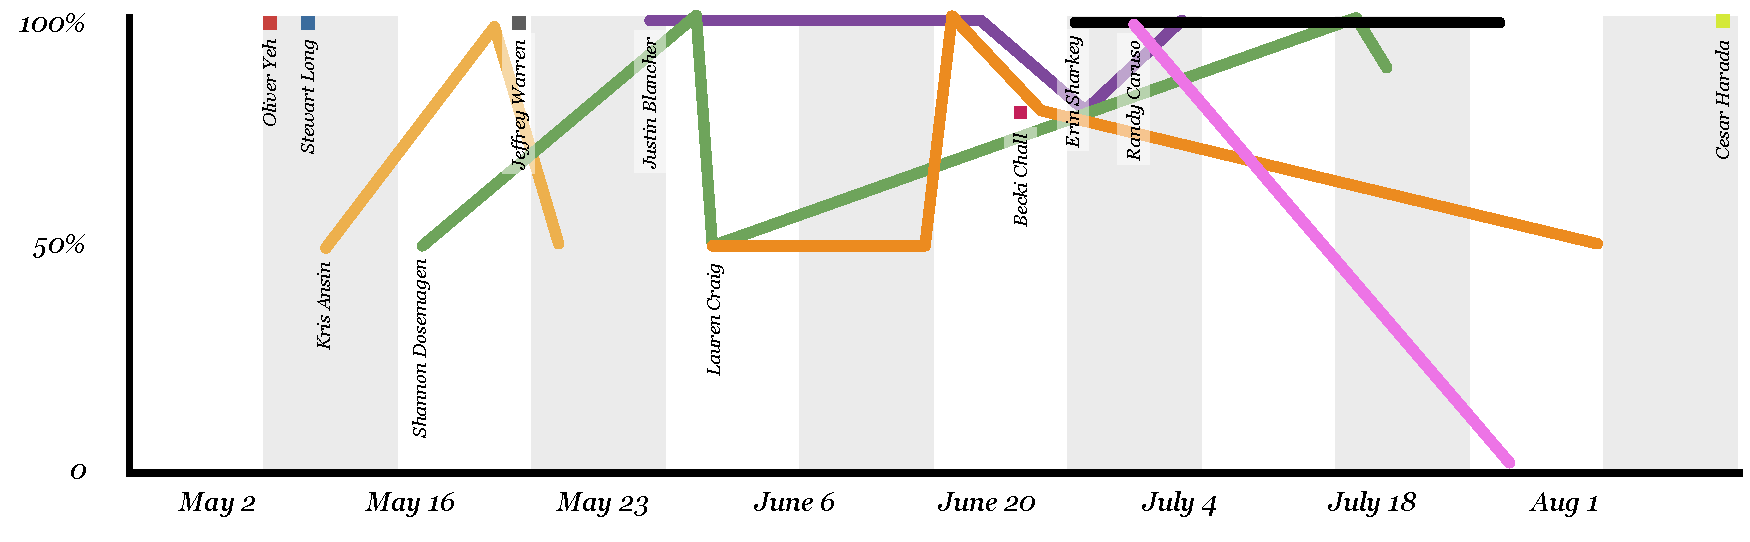
\includegraphics[width=0.45\textwidth]{diagrams/trip-success-leaders.pdf}
		\caption{Success of mapping trips, based on evaluation of resulting imagery by GonzoEarth}
	\end{flushright}
\end{wrapfigure}



\begin{table}[tp] 
\caption{Success of image capture in varying weather conditions during over 33 mapping trips led by \ac{LABB} and other Grassroots Mapping volunteers between May 7th and July 22nd, 2010.}

\label{fig:weathertable}\centering %
\rowcolors{1}{tableShade}{white}
\renewcommand{\arraystretch}{1.0}
\begin{tabularx}{\textwidth}{lYYY}
\toprule\hiderowcolors
Conditions&Balloon or Kite&\# of images&Est. max altitude (ft)\\\otoprule\showrowcolors
&balloon&222&1500\\
&kite&184&\\
&kite&54&\\
&balloon&318&\\
steady wind grew to 20 mph&kite&200&1000\\
&balloon&118&\\
&balloon&182&\\
windy&balloon&100&350\\
very windy&kite&&300\\
good wind&kite&&1000\\
lots of wind&kite&&1000\\
good wind&kite&&1000\\
good&balloon&124&750\\
good&balloon&&350\\
7-8 mph&balloon&362&300\\
poor wind&kite&&500\\
very windy&both&213&1000/1000\\
good&balloon&&800\\
&balloon&665&700\\
stormy&balloon&&1000\\
low wind&kite&&200\\
7-8 mph&balloon&&400\\
very windy&kite&&\\
windy&kite&472&350\\
low wind&both&166&\\
windy&kite&398&350\\
&kite&200&\\
mild steady wind&balloon&323&400\\
difficult wind&balloon&1000&500\\
&balloon&900&300-600\\
wind in wrong direction&balloon&50&500\\
&kite&325&\\
good wind&balloon&971&1000\\
\bottomrule
\end{tabularx}
\end{table}

45\% kite, 55\% balloon
725 ft average balloon altitude over 14 reported
670 ft average kite altitude over 10 reported


\begin{table}[tp] 
\caption{Comparison of maps produced in January 2010 project in Lima, Peru with those available in Google Maps for same period.} 

\label{fig:gulfmapstable}\centering %
\rowcolors{1}{tableShade}{white}
\renewcommand{\arraystretch}{1.4}
\begin{tabularx}{\textwidth}{>{\bfseries}rlYYYYYY}
\toprule\hiderowcolors
Site&Coordinates&Date of capture&Resolution&Area&Trip Leader&Estimated altitude&Technique\\\otoprule\showrowcolors
Grand Isle State Park&&&&&&&\\\hline
Grand Isle State Park&&&&&&&\\
\bottomrule
\end{tabularx}
\end{table}

(Metadata)

\section{Licensing and data use}

The assembly of a public domain archive of data, including \ac{GeoTIFF}s, \ac{TMS} and raw images, is a valuable goal in itself. Due to increased mapping activity after the Katrina disaster, much imagery of the coast already existed, however not at such good resolution. Our inclusion of pre-spill imagery will, as participant Adam Griffith put it, `remind us what the land should look like'. \cite{griffith2010isle} The post-spill maps will help to identify and assess the environmental and economic damage which coastal ecologies and communities have sustained.  
 
The project is ongoing, and even after our current funding and timeline end in January, there is potential to perform ongoing mapping at longer intervals. While the immediate needs of providing imagery to the public and the media have been met, our longer term goals of using the data for litigation and environmental monitoring will require collaboration with those communities, and plans are already in motion to present the data at relevant venues. 

Our choice of a blanket public domain policy has meant that with the exception of some donated imagery, all our data has been released into the public domain and may be downloaded and republished without permission. We expect this to facilitate its adoption by researchers, litigators, and other activists, just as it has amongst the media. Already, images have been republished by the Boston Globe, the New York Times, and many other news agencies. Much of the data has even be licensed to Google for use in the Google Earth and Google Maps products. This reversal --- small organizations providing imagery to Google instead of the opposite --- stands in contrast to the licensing bottleneck which caused so much trouble in the Haiti aid community, as discussed in Section \ref{subsec:satelliterelease}. 

As more such projects unfold\footnote{See Chapter \ref{sec:ongoinguses}}, I hope that the successes we have had in the Gulf Coast will not only provide a wealth of relevant information for other would-be mappers, but that our work will inspire others to adopt these practices in new and interesting ways.  

\chapter{Evaluation}

In assessing the Grassroots Mapping project, I wanted to consider not only the technical merits of the tools and their immediate use, but the success of the project as a human endeavor, and in terms of its effects on the communities involved. While there are important quantifiable benefits to the balloon- and kite-based techniques for capturing imagery and the web-based tools for processing and publishing that imagery, it is also important to address the degree to which the tools were appropriate for participating communities, and whether they felt that the tools served their needs. 

\begin{itemize}
\item Did our maps provide better imagery/information to groups in need?
\item Were the tools adopted and used? Are they financially and technically within reach of the participant communities? 
\item Did participants come to believe in the importance of authoring maps and the rhetorical power of mapping?
\item Did the mapmaking and the ability to make maps affect change in the participant communities?
\item Were the maps uesd in legal processes? Did they help participants advance an agenda? Did they provide critical information?
\end{itemize}

\section{Participants vs. collaborators}

%        Role of Carla, Escuelab, Shuawa
%        Hector as a fellow educator (interview)

\section{Validity in openly ideological research}
\label{sec:lather}

Many of my research questions are qualitative in nature, such as `Did the maps cause participants to re-evaluate their understanding of their environment in political or environmental terms?' or `Did mapmaking change participants' assumptions about what information they could access or utilize to further their interests?' The answers to these questions are profoundly affected by my advocacy of these tools and techniques in the communities with whom I collaborated --- and the degree to which I was able to convince participants to adopt these tools and the beliefs about cartography which they embody. In order to better understand the outcomes of my research, given such an ideological investment by myself and other participants, a degree of reflexivity is required. I therefore look to Patti Lather in her esssay entitled `Reconceptualizing Validity' (p.67) where she outlines a framework for assessing validity in the context of openly ideological research. Such an approach is especially appropriate for a discipline which is increasingly understood as a qualitative field; see Section \ref{sec:gis} for additional discussion on how maps are constructed and the importance of a mixed-methods approach. 

Lather advocates a `vigorously self-aware' regimen of research techniques which she presents in contrast to `positivist' traditional practices which claim objectivity and neutrality. In the face of similar traditional cartographic claims, it is appropriate and productive to apply Lather's four major proposed evaluative methodologies: construct validity, face validity, catalytic validity, and triangulation. 

\subsubsection{Construct validity}

Construct validity refers to how theory was affected by gathered data and by the human realities of the research site or context. In the case of the Grassroots Mapping case studies, the variety of sites we attempted to map, and the time, cost, materials availability, and mapping goals we established with local partners at each sitedictated how we applied these technologies to specific problems. The process of making maps in these places and with these people also brought to light new ways of using and thinking about maps which has gradually changed how I approach map-making and present it to others. Most of all, there was a continual re-negotiation of \textbf{why} we made maps due to political, social, environmental, and economic context. This led to a shift from technological justifications such as higher resolution, better precision, and the more abstract beliefs in `open geodata' to more site-specific reasoning, as well as one which placed greater emphasis on non-quantitative results.  

In Lima, Peru, we expected our claim that we could produce higher resolution imagery than available in Google Maps to inspire or incentivize participants; however most of the youth we were working with were unfamiliar with Google Maps, and comparisons did not resonate as strongly as we had hoped. However, the ability to see oneself in many of the aerial images resonated strongly with participants of all ages. The intent of our mapping work became more tactical, and more aggressive at times --- while these tools were originally designed to help communities map themselves, in Rock Creek, West Virginia, we used balloon mapping to gather data about a mining site operated by Massey Energy; a hostile organization. Members of Coal River Mountain Watch considered the land to be `theirs' in the sense that Massey had gained access to the site through a long history of permit and land ownership manipulations, and the map-making was intended to document what the company was doing `to Appalachia' and the communities surrounding the site.

(redefinition of main challenges - collaboration and integration - move towards illustrated guides, workshops, collaborations)

Perhaps the greatest change has been the application of Grassroots Mapping tools to ever-broader needs, starting with land tenure claims, and growing to include street mapping in Georgia, youth curricula in Boston, Lima, and the West Bank, and environmental monitoring in a wide variety of sites. In the Gulf of Mexico following the 2010 BP oil spill, the realization that our maps were detailed enough to see individual animals and plants became one of the most compelling reasons for the map-making, as did the ability to see ourselves in many images, connected to the camera by the 2000-foot tether. These discoveries broadened the scope of the map-making and affected which sites were targeted. In general, Grassroots Mapping has been slowly repositioned as a source for both ecologically relevant information at a high frequency of capture, and symbolically relevant imagery of events at a human scale.

\begin{wrapfigure}{r}{0.5\textwidth}
  \begin{flushleft}
	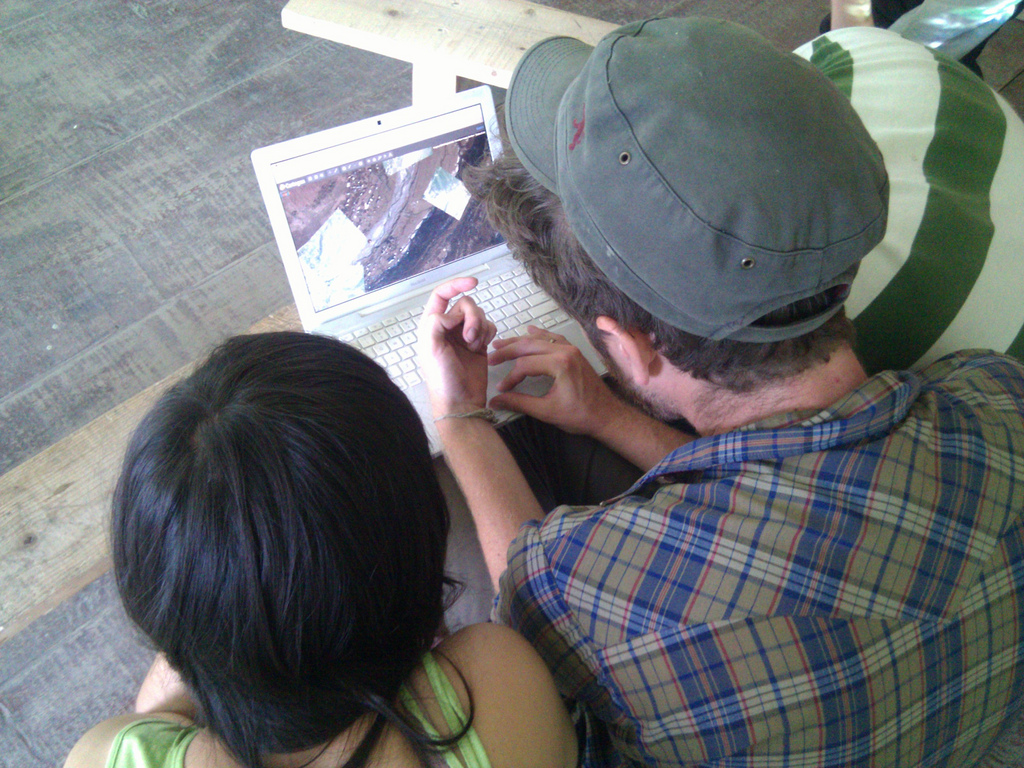
\includegraphics[width=0.5\textwidth]{images/knitter-mestia.jpg} 
	\caption{Austin Cowley of OpenMapsCaucasus and a student from Mestia, Georgia use Cartagen Knitter to join images gathered the day before from a balloon.}
  \end{flushleft}
\end{wrapfigure}

\subsubsection{Face validity}

The importance of creating a feedback loop wherein research output is reviewed and interpreted in collaboration with participants cannot be overstated, and this is the focus of `face validity' as described by Lather. In Grassroots Mapping case studies, I have made every effort to process, analyze, and publish data in a participatory manner --- teaching and demonstrating image selection, orthorectification tools, and discussing the pros and cons of output formats such as printed or digital maps. One of the major components of the toolkit I have developed, the Cartagen Knitter, is specifically intended to aid in the production of maps and to be a sustainable and reproducible means of creating maps with aerial imagery. I have been lucky enough to be able to iteratively test Knitter with participants of varying levels of technical literacy, and to make incremental improvements on the tool's interface and abilities.  

(distribution and analysis of maps themselves, illustration of presentation of maps at JP2)

\begin{wrapfigure}{r}{0.5\textwidth}
  \begin{flushright}
	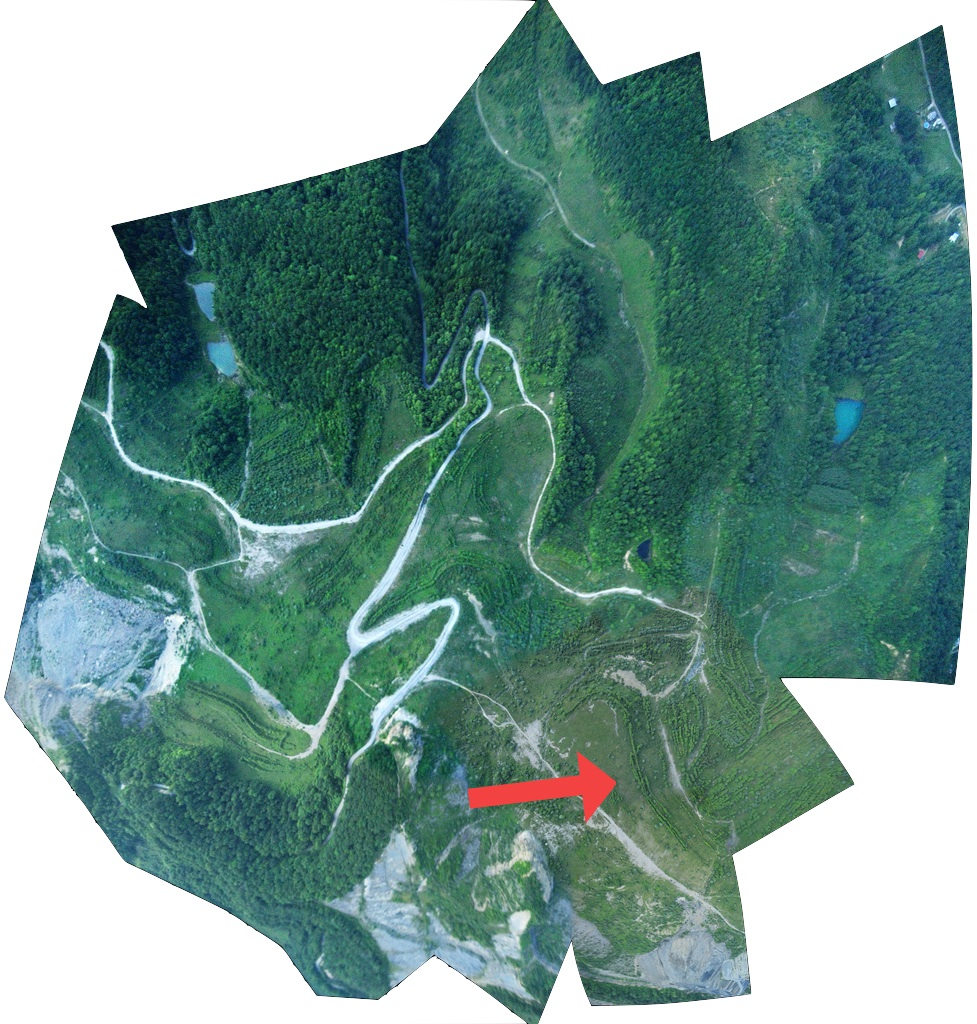
\includegraphics[width=0.5\textwidth]{images/black-mountain.jpg}
	\caption{Roadside plantings at Black Mountain, Virginia}
  \end{flushright}
\end{wrapfigure}

Ultimately, the use of maps to further the interests of participant communities lays in the hands of those participants, and over a longer timeline of months and years, it remains to be seen whether the maps I have produced with people are, for example, submitted as part of a land claim in Lima, Peru, or used to challenge a mining permit in Rock Creek, West Virginia. However, the interpretation of map data by local participants has been an essential component of the project. In a map of Black Mountain, Virginia, however, initial images of a reclamation site appeared in vibrant green when compared to previous data from Google Earth. Since the goal of the map-making was to highlight the environmental degradation the site had sustained, this was concerning, and indeed, upon first seeing the map many people comment on how beautiful the color is. Members of the Coal River Mountain Watch organization pointed out that despite the color, the main points of interest in the data are the contrast between the naturally forested areas and the sparse vegetation which had been replanted, as well as the tendency of the replantings to follow roadways --- the implication being that the mining company tried to mask the damage by planting where people would see it most.  

Specific wording employed by participants has hinted at the degree to which participants took ownership of the process and the resulting maps. Helder Solari, a member of the Escuelab team I worked with in Canta Gallo in Lima, Peru, tellingly referred to the map as `tuyo', or yours, when he wrote to ask for a digital version. I had left only paper copies with leaders of Canta Gallo. He did make reference to the fact that our map (as I describe it) is the only one which shows the Canta Gallo community, pointing out that `in other maps, it simply doesn't exist' \cite{solari2010cantagallo}

(face validity in the Gulf project. draw on writings of participants: lauren craig, shannon, LABB blog, cesar harada)

\begin{quote}
The simplicity of this project is what initially sparked my interest in it. The kits are assembled from relatively inexpensive materials, and almost anyone can perform the basic tasks of attaching the camera and letting out the kite or balloon. --- Lauren Craig
\end{quote}

\begin{quote}
Even though we can’t all be paragliding aerial photographers, wildlife experts or boat captains, we still have a role to play in raising awareness about the effects of this disaster. The best thing that ordinary people can do for the community right now is stay informed, promote action and spread the word—this is the mission of the Louisiana Bucket Brigade in Grand Isle.
--- Lauren Craig, Tulane
\end{quote}
\subsubsection{Catalytic Validity}

One of the most important outcomes of the Grassroots Mapping project is how it has changed participants' assumptions of what kind of information they are able to collect. This is a key aspect of what Lather refers to as \textbf{catalytic validity}, `the degree to which the research process re-orients, focusses, and energizes participants'. In the case of the 2010 BP oil spill, most organizations I spoke with initially did not understand what I meant by mapping --- their response to the spill simply did not take into account the possibility that new aerial data could be captured without a satellite or an aircraft. 

This moment of inspiration can be frustratingly ..... In Lima, Peru, mapmaking is performed by civil engineering firms using traditional surveying techniques. At one point, we were engaged in a mapping exercise with youth from the Canta Gallo community, when leaders of the group came in to the same room to have a meeting with one such firm over the progress of their map! Despite having shown previous maps I had made with other communities, none of the leaders seemed to be interested in applying the techniques towards their apparently immediate needs.  

Most of the groups I have worked with experience a moment of excited inspiration upon seeing the first images of their own site, fresh off of a balloon flight. 

rock creek doubts, later buy-in "We should order a bunch of weather balloons right now!"

\subsubsection{Triangulation}

Press using our images/maps
Google licensing our imagery

\subsection{Interviews with local partners}
Wiki, mailing list, blog, media coverage (~ Face validity)

\section{Comparison with existing techniques}

% possible table of comparison... based on Stewarts?

One of the most compelling aspects of the balloon and kite mapping techniques was its low cost; many of the communities I worked with, including those in Canta Gallo, Lima, and Rock Creek, West Virginia, mentioned cost in particular as a motivation to try these tools. For volunteers at the Louisiana Bucket Brigade in New Orleans, it was the low cost of a mapping kit which made it possible to scale up mapping efforts to several teams, with new maps made every few days, all within a budget of only a few thousand dollars. This made kite and balloon imaging techniques feasible at low cost even before the availability of digital cameras and image manipulation tools; today the development of higher-performance kites, lighter cameras, and open source mapping software has made it even more practical. In particular, the absence of engine noise makes both kite and balloon photography more appropriate than imaging from aircraft for sensitive environmental applications such as observing wildlife without disturbing it. \cite{aber1999kite} In my own work, this was useful while mapping the BP oil spill's affects on birds and other wildlife in the Gulf of Mexico. It has also proven relevant for politically and militarily sensitive areas such as coal mining sites in Appalachia, refugee camps in Palestine.

Image of birds on Chandeleur islands, and helicopter scaring them away.  

Compared to the alternatives, of hiring pilots and paying for fuel and aircraft, or purchasing satellite imagery, balloon and kite mapping seemed not only inexpensive, but more legible and participatory. The idea that one would have to send a camera into space to photograph things which are right next to oneself seems strange, especially when the area of interest is on the scale of a small community. Imagery taken from only 2-4000 feet preserves a sense of the human scale; mappers can often see themselves or their boat or car in the images, and the occasional photograph shows the balloon or kite string leading down from the camera to the ground. This leaves a powerful impression on mappers, who are literally holding the camera in their hand at thousands of feet in the air... albeit at the end of a string. To them, the millimeter-thick string is both a literal and symbolic link to the camera, a reminder of their control over the image and the authorship they have in the resulting map.  

\begin{wrapfigure}{r}{0.5\textwidth}
	\begin{flushright}
		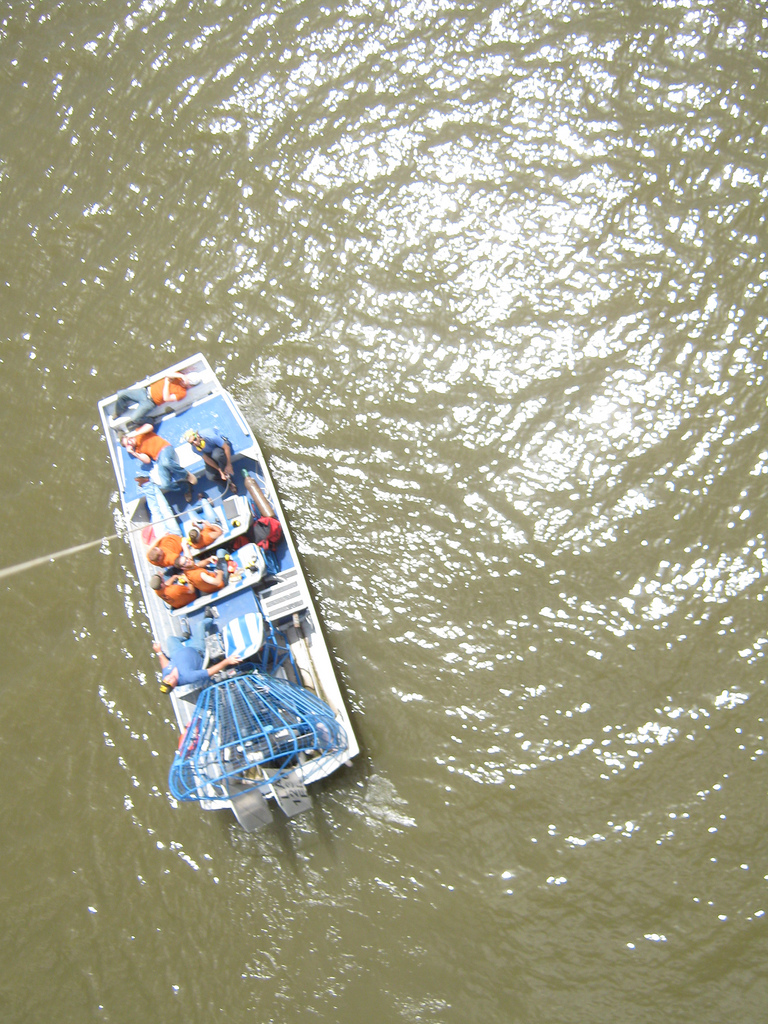
\includegraphics[width=0.45\textwidth]{images/labb-bay-jimmy.jpg}
		\caption{Grassroots mappers in a fanboat at Bay Jimmy, LA on July 22. Photo courtesy Cesar Harada/LABB.}
	\end{flushright}
\end{wrapfigure}

In pragmatic terms, rather than relying on an outside source of expertise, members of participating communities felt that they could perform the image collection themselves, at times of their choosing, and could repeat the imaging at higher intervals than what would be possible with aircraft or satellites. After performing several 'trips' with members of the Louisiana Bucket Brigade and members of Coal River Mountain Watch, participants from those organizations felt comfortable launching their own balloons under observation by myself or Stewart Long, another grassroots cartographer. Several of these participants went on to lead their own trips and bring back their own imagery.

\begin{quote}
In parallel came the discovery that local people could readily interpret black and white aerial photographs, often at 1:5000 (Dewees 1989; Mearns 1989; Sandford 1989). 
\cite{chambers2006participatory}
\end{quote}


\section{Quantitative evaluation}

% how to reconcile this with the Tool chain section

\subsection{Spatial resolution}

Resolution can be measured in the spatial, temoral, and spectral axes; spatial refers to distance in x,y,z in the physical world, temporal refers to the frequency of image capture, and spectral resolution is the amount of color information preserved in an image. Spatial resolution in aerial imagery is referred to in terms of meters or centimeters per pixel; that is, how many meters or centimeters in the real world correspond to the width or height of a single (presumably square) pixel in the photographic data. For example, typical resolution in Google Maps for urban areas in the United States is approximately 1-2 meters. 
 
On a purely technical basis, there were several key benefits to to the techniques employed by the Grassroots Mapping project. In terms of spatial resolution, the typical balloon or kite map ranges from 2-150 cm in resolution, depending on the camera used, the camera altitude, and the desired output resolution. This bridges an important gap in publicly accessible aerial imagery, as commercial satellites today are limited by US law to 50 cm resolution, and the GeoEye 1 satellite, which offers the best current resolution, offers only 141 cm color imagery. This is especially important in environmental applications; Vierling et al emphasize in their use of balloon imagery that `...there still exists a gap between canopy scale processes and landscape level satellite remote sensing measurement.' \cite{vierling2006short} The resolution required to identify objects on the ground is typically three to five times smaller than the target objects, so to identify an object 10 cm wide, a resolution of 2-3 cm is required. \cite{aber2002unmanned} This is a reasonable target resolution for balloon and kite imagery. 

(Cite Remote Sensing table)

% cite GeoEye resolution

\begin{figure}[h]
  \begin{center}
	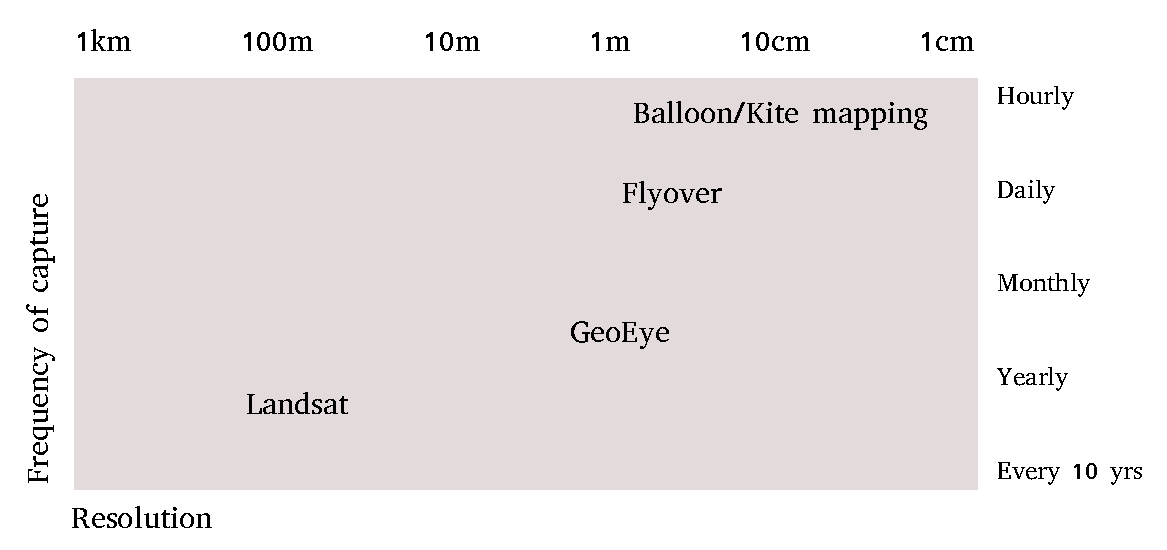
\includegraphics[width=1\textwidth]{diagrams/resolution-frequency.pdf}
	\caption{Comparison of various imaging techniques and typical resolution/frequency characteristics}
  \end{center}
\end{figure}

This is accentuated by the lack of control over the time imagery is captured. Purchasing existing satellite imagery is expensive, at about US\$ 15 per square kilometer (cite Mikel or his sources) but to buy new imagery requires waiting for a satellite to pass over the target area, or even for operators to actually repoint the satellite in space, and thus is even more costly. In the citizen mapping of the BP oil spill in 2010, daily imagery of the spill was available only from the NASA satellites Terra and Aqua, whose MODIS imaging sensor captured a resolution of only 1 km --- though each image could capture the entire oil spill. The images were further obscured by cloud cover (a common challenge with satellite imagery \cite{miyamoto2004use}) and glare from the sun, although I emphasize that the MODIS imagery is extremely useful for different reasons than those captured by balloon or kite; volunteers at the Louisiana Bucket Brigade often used MODIS imagery to identify likely sites to perform kite and balloon mapping. In fact, the two resolutions are almost impossible to reconcile, as all of the citizen maps produced by the Bucket Brigade fit within one or two pixels of the MODIS data. (see illustration)

% find pricing citation
% image of one of our maps overlaid on MODIS imagery

The capture resolution is, of course, a compromise between the desired surface area of coverage and the desired resolution. For example, if a balloon is flown at 1200 meters above the ground, a typical 5 megapixel point and shoot camera will capture an area approximately 1000 meters square \textbf{per photograph} at a resolution of approximately 40 cm. To double that resolution would require flying the balloon at an altitude of approximately 800 meters. In either case, a viable way to increase coverage is to move around with the tether on the ground, either by walking or in a boat or other vehicle. This has the disadvantage of taking a lot of time --- in the above example of flying at 1200 meters, to double the resolution would require walking roughly a kilometer in any direction. This is further complicated by obstacles such as closely spaced trees, power lines, etc.

Human scale --- This considerably better resolution than is typically available makes it possible to produce maps that relate to the human scale; 

\begin{wrapfigure}{r}{0.5\textwidth}
	\begin{flushright}
		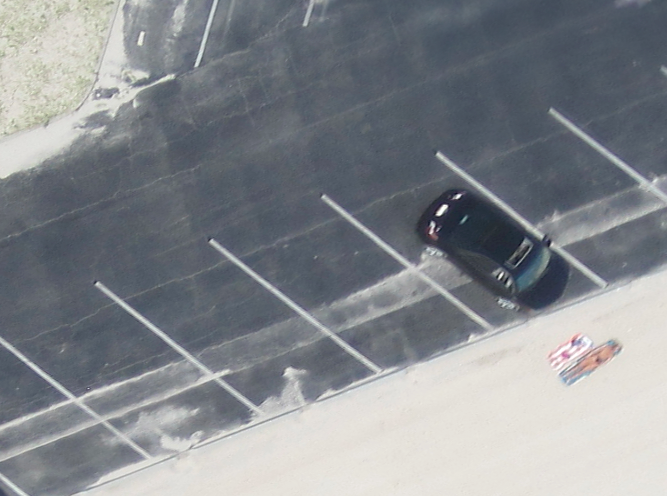
\includegraphics[width=0.45\textwidth]{images/long-beach-sunbathers.png}
		\caption{Mathew Lippincott tests plastic sheeting for porosity to helium after a discussion on the Grassroots Mapping mailing list. \cite{lippincott2010helium}}
	\end{flushright}
\end{wrapfigure}

\subsection{Precision and accuracy in low-altitude aerial imaging}
\label{subsec:precision}

Another important aspect of quantifying spatial resolution is to distinguish the internal precision of an image mosaic and the accuracy of that data compared to the real world. That is, while imagery may be highly spatially consistent in that the location of features relative to one another closely matches reality, the entire image may not be spatially correlated to the real world, and the latitude and longitude positions of those features may vary from their real-world counterparts. This may occur when an image mosaic is assembled from source images with large overlapping areas, and is internally consistent, but cannot be related to the real world due to poor GPS measurements or poor reference map data. Images are typically orthorectified against reference map data of a lower resolution, thus limiting accuracy to the resolution of that source. Eric Wolf makes ...

% Eric Wolf's thesis on BAP metrics: wolf-eric-thesis.pdf

misalignment due to 1) placement of ground targets, 2) photographic distortions, 3) in miyamoto
camera distortion = 4\% in miyamoto

\subsection{Temporal resolution}

Though \textbf{some} satellite imagery is publicly available for virtually every place in the world, and often at useful resolution, even those areas which are mapped at better than 1 meter resolution are often years out of date. There is simply no business case for many satellite imagery providers to capture imagery of many places in the world, and it is impossible to know when the next available dataset will be published, or under what terms. \cite{oconnor2008maps} The ability to \textbf{repeatedly} image an area at intervals of one's choosing makes balloon and kite mapping techniques useful for time-sensitive purposes such as periodically monitoring the effects of the Gulf oil spill (see Chapter \ref{chap:gulf}) or measuring vegetative regrowth in mountaintop removal mining sites undergoing reclamation (see Section \ref{sec:ongoinguses}). 

\subsection{Spectral resolution}

Aerial imagery taken from low altitutdes (under 4000 ft) typically has better color saturation and greater spectral resolution is preserved compared to imagery captured from space or from higher altitude aircraft platforms. This is partly because it is normally captured from below the level of the clouds. (see illustration) This can be significant for environmental assessment, as is the ability to get uncompressed RAW format image data; Crispen Wilson of Conservasi, a  member of the Grassroots Mapping mailing list, is attempting to do spectral analysis of aerial imagery over water. Most aerial or satellite imagery is published as PNG or JPEG tiles, and is not useful for such purposes.  

% back this up... spectral resolution and altitude
% histogram illustrations
% Stewart Long's Chandeleur imagery vs balloon imagery, spectra

Spectral resolution is important for identification of vegetation, and Miyamoto et al have achieved classification of vegetation into 27 different types such as `moss with alpine plants' and 'moss bogs with pools', using 15 cm imagery. They also assert their belief that balloon aerial photography may be used to allow classification to the genus and species level. \cite{miyamoto2004use} Their work has obvious relevance to both the citizen mapping of the BP oil spill (see Chapter \ref{chap:gulf}) and Coal River Mountain Watch's mapping of mountaintop removal mining reclamation sites (see Section \ref{sec:ongoinguses}).

\chapter{Conclusion and future work}

\section{Ongoing uses of Grassroots Mapping tools}
\label{sec:ongoinguses}

\subsection{Activist mapping with Coal River Mountain Watch}

A variety of new projects have been initiated both with and without my prompting or intervention, in order to apply Grassroots Mapping tools towards different goals. One which I had the pleasure of collaborating on directly was a mapmaking pilot project with the Coal River Mountain Watch (CRMW) community, an activist and advocacy organization based in Rock Creek, West Virginia. CRMW works to educate and disseminate information about mountaintop removal mining (MTR) practices in Appalachia, in which companies such as Massey Energy remove entire mountaintops to access coal seams, depositing the `waste' rock in nearby valleys. What results is extreme environmental degradation and a variey of health hazards from water table contamination, landslides, and particulate air pollution. CRMW was interested in using balloons, kites, and remote controlled airplanes. 

% Marsh Fork Elementary map

In collaboration with Stewart Long of \url{http://GonzoEarth.com}, I joined photographer Chris Eichler in attending the Mountain Justice conference at ..... Kentucky. There and subsequently in Marsh Fork, West Virginia, we created a series of maps of mining-related sites. Our first, pictured above, depicts the bright green of a reclamation site, where a mining company has attempted to replant a former MTR site. Rob Goodwin of CRMW and other activists who performed the mapping pointed out that the green color is due to a thin layer of invasive weed which is sprayed over reclamation sites from airplanes. The coverage is thin and there is little or no topsoil over what is essentially a pile of broken-up rock. Aerial imagery shows the contrast between this kind of so-called replanting and the natural forest surrounding the site. It also depicts several contaminated ponds and highlights the tendency of mining companies to plant bushes and shrubs mainly along roadways. 

At the Marsh Fork Elementary school near CRMW headquarters, we launched a balloon to over 4000 feet above ground level, breaking all our previous records for altitude, and captured photos of a runoff pond and an active mining site above the school. By using an electric power drill to reel in the tether, we reduced deployment time, though in that case we ran out of battery for the drill and were forced to revert to hand-reeling. The potential to do power-assisted reeling makes such high-altitude flights more reasonable in a limited time frame, allowing for shorter intervals between flights. With enough power to run a drill, over 1000 feet can be reeled in every 2 minutes. 

An additional advantage to balloon imagery is that it can be captured inconspicuously from public roads upwind of target sites. These tools provide groups such as CRMW access to time-sensitive information about the progressive degradation of the environment, and CRMW hopes to use the data in court cases to prevent mining operations.

\subsection{A Grassroots Mapping collaboration in Georgia}
\label{subsec:georgia}

In early 2010, Jeff Haack of JumpStart International, the nonprofit group which funded and operated the Free Map Palestine project with Mikel Maron in 2008-9, expressed interest in applying Grassroots Mapping tools and ideas to a nation-wide mapping project in the country of Georgia. With educational projects in 5 cities across the country, this was to be the first large explicitly educational application of the Grassroots Mapping concept. Beginning in June 2010 and lasting 6 weeks, the program consisted of a series of workshops and trainings with JumpStart-affiliated educators and activists using balloons and kites.

emphasis on ownership, side effects of skills acquisition and culture of open-source/civil society

\begin{quote}The NGO structure JumpStart has built in Georgia is, in my opinion, an apt and sustainable way forward. After our experience in Palestine it became clear that impact requires a lasting effort in a community and the encouragement of local skills and ownership. It’s not merely about mapping a country, but about understanding where that, conceptually, meets societal needs, and building value therein. Sustainability for OpenMapsCaucasus comes by understanding the convergence of digital technologies with community mapping, social fabric, governance, and civil society, and filling a need within that sphere. We’re not expecting OMC’s community mapping focus to last forever, but that concept, at the very heart of it is meaningful and sustainable, because accessing the tools for extracting and considering not oil or timber, but information, strengthens a society and can make it more prone to long term development.\end{quote} \url{http://brainoff.com/weblog/2010/04/28/1556}

high altitude and extent records, Mestia

\section{Wiki, blog and mailing list}

(redundant with end of tool chain section)

Some community participants have gone to great lengths to document their design iterations and innovations through video, still image, and textual publication. Pat Coyle of Belize Open Source produced several videos of variations on the soda bottle enclosure for cameras, narrating his proposed additions such as a bungee cord to hold the camera tightly against the bottle. Others have posted suggestions for improvements on the camera suspension to stabilize the camera platform, and Mathew Lippincott published an analysis of the permeability of different HDPE thicknesses and pigmentations, in order to identify which is most suitable for use in home-made helium balloons.

% stills from Pat's videos
% Check Pat's bio, BelizeOpenSource...?
% Mathew Lippincott's blog post on helium and HDPE

\begin{wrapfigure}{r}{0.5\textwidth}
	\begin{flushright}
		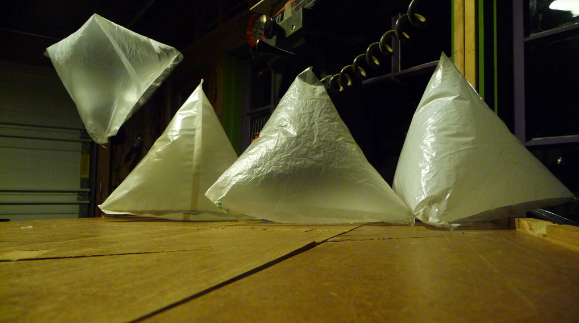
\includegraphics[width=0.45\textwidth]{images/mathew-lippincott-balloons.png}
		\caption{Mathew Lippincott tests plastic sheeting for porosity to helium after a discussion on the Grassroots Mapping mailing list. \cite{lippincott2010helium}}
	\end{flushright}
\end{wrapfigure}


\section{Illustrated Guides}
\label{sec:guide}

Originally suggested on the Grassroots Mapping mailing list in ....... by list member Pat Coyle, the idea of an illustrated guide to provide a rich and cross-language instruction set has received some attention. Storyboarding, outlining, and initial sketches were begun in the spring of 2010 by Pay Coyle, Nathan Cooke of MIT's D-Lab, 

Crispen Wilson or Peter Poole asked for a guide.... find the email

The 4-page PDF guide developed for the Louisiana Bucket Brigade was a quick attempt to provide such instructions, but was primarily intended to serve as an organizational guide and checklist, with tips and reminders, rather than a complete start-to-finish guide. 

For those interested in learning or teaching Grassroots Mapping techniques, there is also a five page illustrated guide in English, Spanish, Portuguese and Georgian.

\section{Outreach}

There has been a great deal of interest from both technology enthusiasts (kite, RC airplane, and geo-programmers alike) and organizations working in local communities to implement Grassroots Mapping tools and techniques. Part of the ongoing development of this community will be the brokering of relationships between these two communities, and the matchmaking of those with the technical know-how with those in need of geospatial information and training. The Grassroots Mapping mailing list incorporates representatives of both of these groups, and as such will continue to be the central organization point for such collaborations. I plan to organize meetup sessions in key areas to bring these communities together in a hands-on, workshop setting, where personal connections and professional relationships can evolve.

\appendix

\chapter{Maps}

\section{Maps from Lima, Peru}

\subsection{Juan Pablo II}

\subsection{San Ignacio Loyola}

\subsection{Canta Gallo I}

\subsection{Canta Gallo II}

\section{Maps from the 2010 BP Oil Spill}



\section{Maps from Appalachia}

\subsection{Black Mountain, Virginia}

\subsection{Cherry Pond Mountain, West Virginia}

\section{Maps from Georgia}


\chapter{Guides and curricular materials}


\chapter{Materials checklists and prices}

\section{Price lists for balloon, kite, and RC plane mapping kits}

\begin{table}[tp] 
\caption{Grassroots Mapping workflow}
\centering %
\renewcommand{\arraystretch}{1.4}
\begin{tabularx}{\textwidth}{YYY}
\toprule
Capture&Orthorectification&Publication\\\otoprule
2-3 people can map several square km in 1 day&Sorting photos can take \textgreater1 hour, stitching up to 1 day&Export from Cartagen Knitter generates a TMS or printable GeoTiff; only web access is needed.\\\bottomrule 
\end{tabularx}
\end{table}

\chapter{Donors and supporters of the Citizen Mapping of the Oil Spill effort}

The following organizations offered generous support in the form of time, money, transportation, and other means. My thanks go out to them on behalf of everyone involved in the oil spill mapping project. 

\begin{itemize}
\item{Louisiana Bucket Brigade}
\item{GonzoEarth}
\item{1337arts.com}
\item{MIT's Center for Future Civic Media}
\item{The Knight Foundation}
\item{Kris Ansin}
\item{John Norwood}
\item{Adam Boult}
\item{The Lafourche Parish Port Commission}
\item{DevelopmentSeed}
\item{The Washington Post}
\item{TungstenMonkey Productions/Kristian Hansen}
\item{WebMadeMovies/Brett Gaylor}
\item{Jeff Johnson}
\item{Liz Barry}
\item{The Blue Seals}
\item{Uptown Angler}


\end{itemize}

\nocite{*}
{\small
\bibliographystyle{plain}
\bibliography{thesis}
}

\chapter*{Acronyms}

\begin{acronym}
\acro{TMS}{Tiled Map Service}
\acro{GeoTIFF}{Geographic TIFF, or Geographic Tiled Image File Format}
\acro{GSS}{Geographic Stylesheets}
\acro{CHDK}{Canon Hacker Development Kit}
\acro{KAP}{Kite Aerial Photography}
\acro{BAP}{Balloon Aerial Photography}
\acro{COFOPRI}{Organization for the Formalization of Informal Property}
\acro{LABB}{Louisiana Bucket Brigade}
\acro{SVG}{Scalable Vector Graphics}
\acro{JOSM}{Java OpenStreetMap Editor}
\end{acronym}

\chapter*{License}

This work is licensed under the Creative Commons Attribution 3.0 Unported License. To view a copy of this license, visit \url{http://creativecommons.org/licenses/by/3.0/} or send a letter to Creative Commons, 171 Second Street, Suite 300, San Francisco, California, 94105, USA.

\end{document}
